\documentclass[12pt]{report}

\usepackage[a4paper,width=150mm,top=25mm,bottom=25mm,bindingoffset=6mm]{geometry}
\usepackage[onehalfspacing]{setspace}
\usepackage{ucs}
\usepackage[table,xcdraw]{xcolor}
\definecolor{mColor1}{rgb}{0.9,0.9,0.9}

\usepackage{fancyhdr}
\pagestyle{fancy}
\fancyhead{}
\renewcommand{\chaptermark}[1]{\markboth{#1}{}}
\renewcommand\sectionmark[1]{\markright{\thesection\ #1}}

\fancyhead[LO, RE]{\leftmark}
\fancyhead[LE, RO]{\rightmark}

\usepackage{titlesec, blindtext, color}
\definecolor{gray75}{gray}{0.75}
\usepackage{mathptmx}
\usepackage[utf8]{inputenc}
\usepackage[T1]{fontenc}
\usepackage[ngerman]{babel}

\usepackage{amsmath,amssymb,amstext,amsthm,mathtools}
\usepackage{url}
\usepackage{caption}
%\usepackage[belowskip=-5pt,aboveskip=0pt]{caption}
\usepackage{subcaption}

\usepackage{float}
\usepackage{lscape}
\usepackage{pdfpages}
\usepackage{rotating}
\usepackage{graphicx}
\setlength\parindent{0pt}
\usepackage{hyperref}
\usepackage{acronym}
\usepackage{textcmds}
\usepackage{longtable}
\usepackage[export]{adjustbox}
\usepackage{upgreek}
\usepackage{dsfont}
\usepackage{tensor}
\usepackage{amsbsy}
\usepackage{multirow, hhline, colortbl}
\usepackage[table]{xcolor}


\DeclareMathAlphabet{\mathcal}{OMS}{cmsy}{m}{n}
\SetMathAlphabet{\mathcal}{bold}{OMS}{cmsy}{b}{n}

\usepackage{listings, lstautogobble}
\usepackage{textcomp}
\definecolor{yo}{rgb}{0.9,0.6,0}
\definecolor{Gray}{gray}{0.9}
\definecolor{listinggray}{gray}{0.9}
\definecolor{lbcolor}{rgb}{0.95,0.95,0.95}
\definecolor{greylines}{rgb}{0.9529,0.9529,0.9529}

\lstset{
	backgroundcolor=\color{lbcolor},
	tabsize=4,
	rulecolor=,
	language=python,
        basicstyle=\scriptsize,
        upquote=true,
        aboveskip={1.5\baselineskip},
        columns=fixed,
        showstringspaces=false,
        extendedchars=true,
        breaklines=true,
        prebreak = \raisebox{0ex}[0ex][0ex]{\ensuremath{\hookleftarrow}},
        frame=lines,
        showtabs=false,
        showspaces=false,
        showstringspaces=false,
        identifierstyle=\ttfamily,
        keywordstyle=\color[rgb]{0.55,0,0},
        alsoletter={/,*,[,]},%
        otherkeywords={},
        morekeywords=[2]{with, as},
        morekeywords=[3]{},
        emph={self},          % Custom highlighting
		emphstyle=\color[rgb]{0.1,0.3,1},
		emph={[2]f},          % Custom highlighting
		emphstyle={[2]\color[rgb]{0.1,0.5,0.1}},
		emph={[3]__init__},          % Custom highlighting
		emphstyle={[3]\color[rgb]{0.1,0.3,1}},
		emph={[4]open,str,print,KeyError},          % Custom highlighting
		emphstyle={[4]\color[rgb]{0.2,0.6,0.8}},
        commentstyle=\color[rgb]{0.3,0.3,0.3},
        stringstyle=\color[rgb]{0.133,0.545,0.133},
        	autogobble=true
}
\lstnewenvironment{ttlisting}{\lstset{basicstyle=\scriptsize}}{}

\usepackage{color}
\usepackage[section]{placeins}

\newenvironment{simplechar}{%
	\catcode`\$=12
	\catcode`\&=12
	\catcode`\#=12
	\catcode`\^=12
	\catcode`\_=12
	\catcode`\~=12
	\catcode`\%=12
	\catcode`\"=12
	\catcode`\'=12
	}{}{}

\newtheoremstyle{dotless}{}{}{\itshape}{}{\bfseries}{}{ }{}

\theoremstyle{dotless}

\newtheorem{thm}{Theorem}
\newtheorem{defn}[thm]{Definition}
\newtheorem{exmp}[thm]{Example}
\theoremstyle{definition}


\begin{document}

\begin{titlepage}
	Warum bin ich nicht einfach Staubsaugervertreter geworden?
\end{titlepage}

\tableofcontents

\chapter{Zahlungsströme, Versicherungs-, Finanzmarktprodukte und Märkte}

\section{Zahlungsstrommodelle und Wertentwicklungen}

\begin{itemize}
\item Zahlungsstrom auch, wenn nur Werte (Vermögen, Schulden) oder Preise(Kurse) ermittelt werden
\item Nicht monetäre Aspekte: Veräußerungs- und Kündigungsrechte, Entscheidungs- und Informationsrechte
\item Formal Zahlungsstrom (Cash Flow): Menge von finanziellen Größen $Z_t$, wobei $Z_t$ Zahlung zum Zeitpunkt $t$ darstellt
\item Zeitmenge $\mathbb{T}$ ist zu spezifizieren (Bsp.: $\mathbb{T}=\{t_0, ..., t_n\}$
\item Zu beachten, ob Zahlungen vorschüssig (Periodenbeginn) oder nachschüssig (Periodenende) bezahlt werden
\item Im Weiteren: Zahlungsströme sind stochastisch
\end{itemize}

\subsubsection{Definition Stochastischer Prozess}
Es sei $(E, \varepsilon)$ ein messbarer Raum. Ein stochastischer Prozess $X=(X_t)_{t \in \mathbb{T}}$ mit Zustandsraum $(E, \varepsilon)$ ist eine zeitindexierte Familie $E$-wertiger Zufallsvariablen auf messbaren Raum $(\Omega, \mathcal{F})$.


\subsection{Informationsfiltration und adaptierte stochastische Prozesse}

\begin{itemize}
\item Die Bewertung eines Finanztitels zum Zeitpunkt t hängt ab von der in t zur
Verfügung stehenden Information
\begin{itemize}
\item Die zum Zeitpunkt $t$ zur Verfügung stehende Information wird formalisiert
durch eine $\sigma$-Algebra $\mathcal{F}_t$.
\item Die $\sigma$-Algebra $\mathcal{F}_t$ umfasst alle Ereginisse (TM von $\Omega$), die zum Zeitpunkt $t$ bekannt sind, ob sie eingetreten sind oder nicht
\item Da die Information im Zeitverlauf - durch Beobachtung der Realisierungen
von Zahlungen oder Preisen - zunimmt, ist die Folge $\mathbb{F}=(\mathcal{F}_t)_{t \in \mathbb{T}}$ der Sigma-Algebren aufsteigend, d. h. es gilt: $\mathcal{F}_s \subseteq \mathcal{F}_t \subseteq \mathcal{F}$ für alle $s \leq t, t \in \mathbb{T}$
\end{itemize}
\end{itemize}

\subsubsection{Definition Filtration}
Eine aufsteigende Familie $\mathbb{F}=(\mathcal{F}_t)_{t \in \mathbb{T}}$ von Sigma-Algebren heißt Filtration. Das Tupel $(\Omega, \mathcal{F}, \mathbb{F} = (\mathcal{F}_t)_{t \in \mathbb{T}}, \mathbb{P})$ heißt filtrierter
Wahrscheinlichkeitsraum für ein gegebenes Wahrscheinlichkeitsmaß $\mathbb{P}$.

\subsubsection{Definition Adaptierter stochastischer Prozess}
Es sei $(\Omega, \mathcal{F}, \mathbb{F} = (\mathcal{F}_t)_{t \in \mathbb{T}}, \mathbb{P})$ ein filtrierter Wahrscheinlichkeitsraum. Ein
stochastischer Prozess $X=(X_t)_{t \in \mathbb{T}}$ heißt adaptiert an die Filtration $(\mathcal{F}_t)_{t \in \mathbb{T}}$, wenn jede Zufallsvariable $X_t$ $\mathcal{F}_t$-messbar ist.


\section{Charakterisierung von Finanztiteln}

\subsubsection{Realwert vs. Nominalwert}
\begin{itemize}
\item Realwert im Sinne von Sachwert oder Substanzwert zu verstehen.
\begin{itemize}
\item Bspw. Aktien, Immobilien, Edelmetalle (Physicher Wert)
\item Realwerte in diesem Sinne haben einen Wert an sich
\end{itemize}
\item Nominalwert sind typischerweise Geld oder Zinstitel, die nicht immanent einen physischen Wert beinhalten
\item Realwerte sind besser gegen Inflation geschützt
\end{itemize}


\subsection{Zinstitel}
\begin{itemize}
\item Zinstitel (Gläubigertitel) verbriefen eine schuldrechtliche Verpflichtung
(„Kreditaufnahme“) und beinhalten entsprechende Forderungsrechte (Tilgung
der Schuld und terminlich fixierte Zinszahlungen) des Gläubigers
\begin{itemize}
\item Emittenten von Zinstiteln sind bspw. Staaten, Banken oder Industrieunternehmen. ( Government Bonds, Corporate Bonds)
\item Die Zinszahlungen werden als Kupons bezeichnet, die Höhe der Schuld ist der
Nennwert (Face Value).
\item Die Bewertung der Zahlungsfähigkeit (Bonität) des Emittenten erfolgt in Form
eines Ratings (bspw. durch Rating-Agenturen).
\end{itemize}
\item Zinstitel haben feste Laufzeit
\item Vertragsparameter:
\begin{itemize}
\item Der Bond hat einen Fälligkeitszeitpunkt $T$ und Zahlungszeitpunkte $t_i$ $(i = 1,..., n; t_0 < t_1 < ... < t_n = T)$.
\item In $t_0$ erwirbt der Käufer den Bond vom Emittenten zum Preis (Kaufkurs) $P_{t_0}$.
\item Kuponzahlungen erfolgen zu den Zeitpunkten $t_i$, die Rückzahlung der Schuld
(Nennwert) zur Fälligkeit $T$.
\end{itemize}
\item Festzinstitel: Die Zinszahlungen während der Laufzeit erfolgen stets in gleicher unveränderter Höhe
\item Standardbond (Straight Bond)
\begin{itemize}
\item Endfällige Tilgung der Schuld (Nennwert) $N$; konstante jährliche Zinszahlungen
(Kupons) $Z$ der Höhe $Z = N_i$, wobei $i$ den Nominalzins bezeichne
\item Zeitpunkte der Zins- und Tilgungszahlungen sind äquidistant
\item Zahlungsstrom aus Käufer-Sicht: $\{-P(t_0); Z; ... ; Z; Z + N\}$.
\end{itemize}
\item Zerobond (Nullkuponanleihe) bzw. Diskontpapiere (Discount Papers)
\begin{itemize}
\item Eine Nullkuponanleihe bzw. Zerobond ist ein Zinstitel, bei dem keine
Zinszahlungen erfolgen, sondern nur eine endfällige Tilgung.
\item Die wegfallenden Zinszahlungen werden kompensiert durch die Vornahme eines
Abschlags (Diskont) auf den vom Käufer bei Erwerb zu entrichtenden Preis.
\end{itemize}
\item Variabel verzinsliche Titel: Die Zinszahlungen während der Laufzeit erfolgen in veränderlicher Höhe, typischerweise angepasst an die Entwicklung eines Referenzzinses.
\end{itemize}


\section{Aktien}

\begin{itemize}
\item Aktien sind Wertpapiere, die bestimmte Teilhaberechte an einer Aktiengesellschaft (AG) verbriefen (Bspw.: Stimmrecht in der Hauptversammlung, Recht auf Dividende, Recht auf Bezug junger Aktien, Auskunfts- und Anfechtungsrechte)
\item Bei „Nennwertaktien“ wird das Grundkapital der AG
in eine bestimmte Anzahl auf einen festen Nennwert laufende Aktien zerlegt,
mit deren Übernahme ein*e Aktionär*in einen Anteil an der AG erwirbt.
\item Als „Miteigentümer*innen“ der Gesellschaft partizipiert ein*e Aktionär*in
sowohl an einer positiven Entwicklung (Anteil am Gewinn) als auch an einer
negativen Entwicklung (Gewinnausfall, Liquidation). Die Haftung ist jedoch
auf den Verlust des Nennwerts der erworbenen Aktien beschränkt.
\item Nennwert vs. Kurswert:
\begin{itemize}
\item Bei börsengehandelten AGs tritt neben den Nennwert einer Aktie ihr Kurswert.
\item Ein*e Investor*in kann Aktien zu ihrem jeweiligen Kurswert
erwerben/veräußern.
\end{itemize}
\item Zahlungsstrom:
\begin{itemize}
\item Erwerb der Aktie in $t_0$ zu einem (bekannten) Preis (Kaufkurs) $P_{t_0} = s_0$
\item Dividendenzahlungen $D_{t_i}$ zu den Zeitpunkten $t_i$, $(i = 1, ..., n; t_0 < t_1 <... < t_n < T)$
\item Verkauf der Aktie in $T$ zum Preis (Verkaufskurs) $S_T$
\end{itemize}
\end{itemize}


\section{Immobilien}

\begin{figure}[ht]
	\centering
	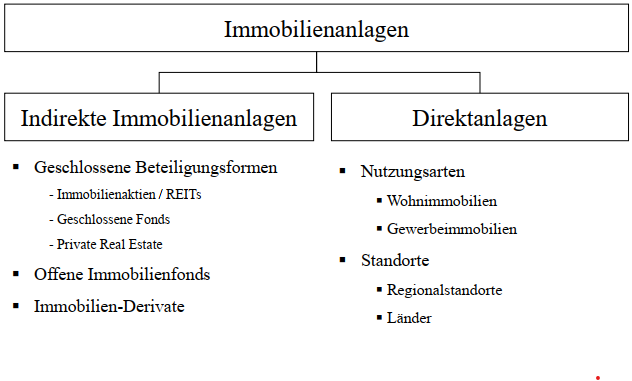
\includegraphics[width= \textwidth]{Bilder/Immobilien.png}
\end{figure}

\begin{itemize}
\item Eigenschaften:
\begin{itemize}
\item Immobilien wird eine hohe reale Wertbeständigkeit (Inflationsschutz!)
zugeschrieben.
\item Feringe Korrelation der Wertentwicklung von Immobilien mit
andern Anlageklassen (Diversifikationspotential!).
\item laufendes Einkommen (Mieten) 
\end{itemize}
\item Nachteile: hohe Eintrittkosten, Illiquidität
\end{itemize}


\section{Derivate}

\begin{itemize}
\item Kassamärkte:
\begin{itemize}
\item Bei einem Kassageschäft wird in einem Zeitpunkt $t = s$ sowohl der Vertrag
abgeschlossen als auch (modulo technischer Frist) der Vertrag erfüllt.
\item Ausgerichtet auf effektive Erfüllung, d. h. der Käufer erhält den zugrunde
liegenden Basistitel und bezahlt den Preis an den Verkäufer.
\end{itemize}
\item Terminmärkte:
\begin{itemize}
\item Bei einem Termingeschäft wird in $t = s$ der Vertrag abgeschlossen, aber
(intendiert) erst in $t = T > s$ („auf Termin“) erfüllt.
\item Ausgerichtet auf effektive Erfüllung oder auf Ausgleich (Zahlung eines
Differenzbetrags) (Cash Settlement).
\item Termingeschäfte müssen stets einen direkten oder indirekten Bezug zu
Kassageschäften (Basistitel, Basisobjekt, Underlying Security) besitzen
(derivative Titel).
\end{itemize}
\end{itemize}



\subsubsection{Formale Charakterisierung:}
Derivative Finanztitel (auch: derivative Finanzinstrumente, Derivate) sind
Finanztitel, deren Zahlungsströme aufgrund vertraglicher Regelungen von den
Zahlungsströmen eines oder mehrerer anderer Finanztitel abhängen. (begriffliches Gegenstück: primäre (auch: originäre) Finanztitel)\\
Motive für Einsatz: Wertsicherung, Spekulation, Arbitrage, Ertragsmehrung

\begin{figure}[ht]
	\centering
	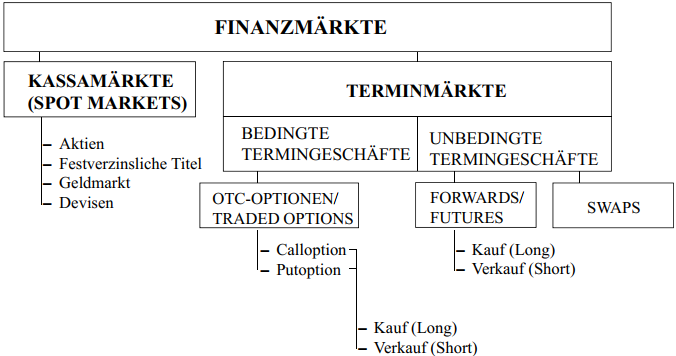
\includegraphics[width= \textwidth]{Bilder/Finanzmarkt.png}
\end{figure}


\subsubsection{Forward-Kontrakt}
\begin{itemize}
\item Ein Forward-Kontrakt beinhaltet für den Käufer (Long Position) bzw. den
Verkäufer (Short Position) die feste Verpflichtung:
\begin{itemize}
\item zu einem bestimmten zukünftigem Zeitpunkt (Liefertermin)
\item unter Zugrundelegung eines vorab vereinbarten Referenzwerts („Preis“) für die
Abrechnung zum Liefertermin
\item einen spezifischen (realen oder synthetischen) Finanztitel (Basistitel,
Underlying) zu kaufen bzw. zu verkaufen bzw. den entsprechenden
Differenzbetrag zu begleichen (Cash Settlement).
\end{itemize}
\item Zahlungsstrom:
\begin{itemize}
\item Erwerb bzw. Verkauf eines Forwards in $t = s$ mit Erfüllungszeitpunkt
$t = T(> s)$:
\item Ein Zahlungsfluss findet nur in $t = T$ statt („Null-Investment“).
\item Höhe: $K_T - F_s$ aus Sicht des Käufers bzw. $F_s - K_T$ aus Sicht des Verkäufers, wobei $K_T$ der Wert des Basistitels des Forwards zum Zeitpunkt $t = T$ und $F_s$ der vereinbarte Referenzwert für die Schlussabrechnung
\item Zahlungsbetrag je nach Kursentwicklung positiv oder negativ.
\item Käufer profitiert von steigenden, Verkäufer von fallenden Kursen des Basistitels.
\end{itemize}
\end{itemize}


\subsection{Optionskontrakte}
\begin{itemize}
\item Eine Option ist ein Vertrag, der dem Käufer (Inhaber der Option) gegen
Zahlung des Optionspreises das Recht - nicht aber die Verpflichtung -
einräumt
\begin{itemize}
\item eine bestimmte Menge (Kontraktvolumen) eines spezifizierten Finanztitels
\item zu einem vorab festgelegten Referenzpreis
\item am Ende (Europäische Option) oder aber auch während (Amerikanische
Option) einer bestimmten Frist
\item zu kaufen (Kaufoption, Call) bzw. zu verkaufen (Verkaufsoption, Put)
\end{itemize}
\item Bei Optionen besitzt nur der Optionskäufer das Ausübungsrecht, der
Verkäufer (Stillhalter) muss auf die Lieferung bzw. Abnahme vorbereitet sein.
Konsequenz: Asymmetrisches Zahlungsprofil
\end{itemize}

\begin{figure}[ht]
	\centering
	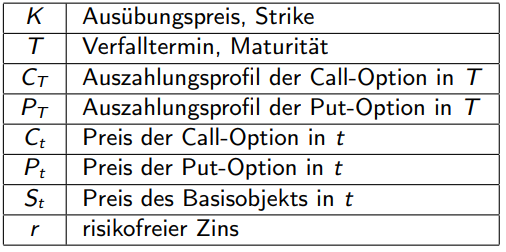
\includegraphics[width=0.7 \textwidth]{Bilder/NotationOption.png}
\end{figure}


\subsubsection{Kauf einer Kaufoption}
\begin{itemize}
\item Käufer: Recht auf Erwerb des Basistitels zum Ausübungspreis $K$
\end{itemize}

\begin{figure}[ht]
	\centering
	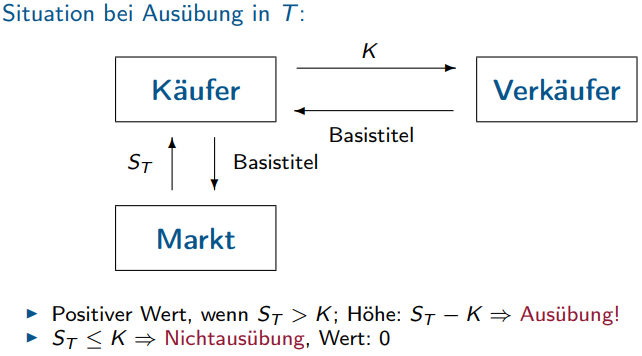
\includegraphics[width=0.7 \textwidth]{Bilder/Kaufoption.png}
\end{figure}

\begin{itemize}
\item Auszahlungsprofil der Call-Option: $C_T = max\{S_T - K, 0\} = (S_T-K)^+$
\item Gewinn/Verlust-Position $G_T$: \\
$C_T=(S_T-K)^+ \Rightarrow G_T=C_T - C_0$ bzw. $G_T=C_T - C_0(1+r)^T$
\item Möglicher Gewinn: unbegrenz, möglicher Verlust: limitiert auf Call-Prämie
\end{itemize}


\subsubsection{Kauf einer Verkaufsoption}
\begin{itemize}
\item Käufer: Recht auf Lieferung des Basistitels zum Ausübungspreis K
\end{itemize}
\vspace{0.3cm}
\begin{figure}[ht]
	\centering
	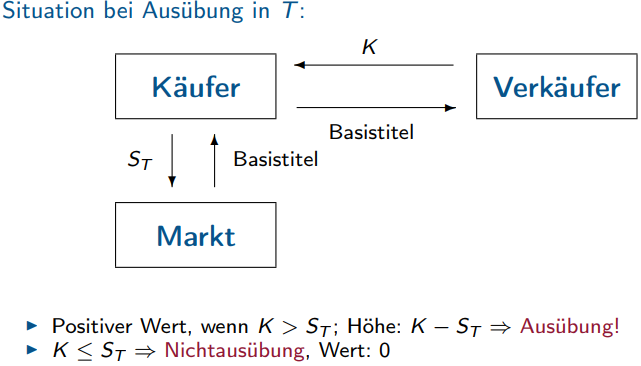
\includegraphics[width=0.7 \textwidth]{Bilder/Verkaufoption.png}
\end{figure}
\vspace{0.3cm}
\begin{itemize}
\item Auszahlungsprofil der Put-Option: $P_T = max \{K-S_T, 0\} = (K-S_T)^+$
\item Gewinn/Verlust-Position $G_T$: \\
$P_T = (K-S_T)^+ \Rightarrow G_T=P_T-P_0$ bzw. $G_T=P_T-P_0(1+r)^T$
\item Möglicher Gewinn: limitiert auf Ausübungspreis minus Put-Prämie
Möglicher Verlust: limitiert auf Put-Prämie
\end{itemize}

\begin{figure}[ht]
	\centering
	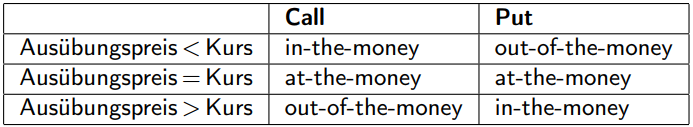
\includegraphics[width=0.7 \textwidth]{Bilder/ImGeld.png}
\end{figure}




\chapter{Grundkonzepte zur Bewertung} 

\section{Bewertung von Zahlungsströmen}

\subsection{Bewertung finanzieller Zahlungsströme - Grundkonzepte im Überblick}


Gegeben sei eine Menge $\mathcal{X}$ von Zufallsvariablen/ Finanzpositionen auf $(\Omega, \mathcal{F})$

\subsubsection{Definition Präferenzordnung}
Eine (vollständige, schwache) Präferenzordnung (Präferenzrelation) auf $\mathcal{X}$ ist eine binäre Relation $\succeq$ mit den folgenden Eigenschaften:
\begin{itemize}
\item Vollständigkeit: Für alle $X, Y \in \mathcal{X}$ gilt entweder $X \succeq Y$ oder $Y \succeq X$ oder beides.
\item Transitivität: Aus $X \succeq Y$ und $Y \succeq Z$ folgt stets $X \succeq Z$.
\end{itemize}

\subsubsection{Definition Präferenzfunktional}
Ein Präferenzfunktional $\mathcal{U}$ zu Präferenzordnung $\succ$ ist eine Abbildung $\mathcal{U} : \mathcal{X} \rightarrow \mathbb{R}$, sodass für alle $X,Y \in \mathcal{X}$ gilt: $X\succ Y \Leftrightarrow \mathcal{U}(X) > \mathcal{U}(Y)$ \\

Beispiel $(\mu, \sigma)$-Prinzip:
\begin{itemize}
\item Das Präferenzfunktional besitzt die Form
\begin{equation}
\mathcal{U}(X) = H(E[X], \sigma(X))
\end{equation}
wobei $H$ typischerweise eine Funktion ist, die in der ersten Komponente
monoton steigend und in der zweiten monoton fallend ist.
\item Wird die Funktion H konkret festgelegt, bspw.
\begin{equation}
H(x,y) = x-ay^2 \text{ mit } a>0
\end{equation}
so wird teilweise auch von der $(\mu, \sigma)$-Regel gesprochen.
\end{itemize}


\subsubsection{Standardrepräsentation von Präferenzfunktionalen}
I.A. untersucht man Bedingungen (Axiome rationalen Verhaltens),
unter denen das Präferenzfunktional U folgende Repräsentation besitzt: $\mathcal{U}(X) = E[u(X)]$

\begin{itemize}
\item Dies wird als von Neumann-Morgenstern-Repräsentation bezeichnet.
\item Die Funktion $u$ heißt (Risiko-)Nutzenfunktion.
\item Die damit verbundene Entscheidungstheorie wird als Erwartungsnutzentheorie
oder als Bernoulli-Prinzip bezeichnet.
\end{itemize}

\subsubsection{Eigenschaften der Risikonutzenfunktion}

\begin{itemize}
\item Monotonie
\begin{itemize}
\item Die Präferenzordnung wird als monoton bezeichnet, wenn ein*e Investor*in für
sichere Auszahlungen $x$ und $y$ mit $x > y$ stets $x$ bevorzugt.
\item Im Fall des Bernoulli-Prinzips ist dies offenbar äquivalent dazu, dass für $x > y$
stets $u(x) > u(y)$ gilt, d. h. die Nutzenfunktion streng monoton steigend ist.
\end{itemize}
\item Risikoeinstellungen
\begin{itemize}
\item Risikoaversion: Die Präferenzordnung wird als (strikt) risikoavers (risikoscheu) bezeichnet, wenn ein*e Investor*in für jede nicht-degenerierte Finanzposition $X \in \mathcal{X}$ die sichere Zahlung in Höhe von $E[X]$
der Zufallszahlung $X$ vorzieht, formal: $E[u(X)]<u(E[X])$
\item Risikoneutralität: $E[u(X)] = u(E[X])$
\item Risikosympathie: $E[u(X)] > u(E[X])$
\end{itemize}
\end{itemize}

\subsubsection{Definition Sicherheitsäquivalent}
Das Sicherheitsäquivalent einer Zufallsvariable X ist derjenige deterministische
Wert $s(X)$, der zu $X$ nutzenäquivalent ist. Formal: $ u(s(X)) = E[u(X)]$ \\

Arrow-Pratt-Maß: $r(x) := -\frac{u''(x)}{u'(x)}$

\subsubsection{Risiko/Wert-Modelle}

Risiko/Wert-Modelle stellen konzeptionell eine Verallgemeinerung des
$\mu, \sigma)$-Prinzips dar. Sie zerlegen den Bewertungsprozess in zwei Stufen:
\begin{itemize}
\item Ein*e Entscheidungsträger*in quantifiziert (isoliert) Risiko $\rho (X)$ und
Wert $V(X)$ von $X$
\item Die Risiko- und Werteinschätzung wird zu einer Gesamtpräferenz
zusammengeführt. Formal: $\mathcal{U}(X) = H(V(X), \rho(X))$
\end{itemize}


\subsubsection{Marktbewertung:}
\begin{itemize}
\item Mark-to-Market: Wird ein Finanztitel an einem Kapitalmarkt gehandelt, so spiegelt der Marktpreis des Titels seine Bewertung durch die Akteure an diesem Markt wider.
\item Mark-to-Model: Ein aktiver Markt existiert nicht oder der Zeitwert kann nicht zuverlässig
ermittelt werden.
\item Ziel einer Marktbewertung auf der Modellebene ist die Ermittlung von
Gleichgewichtspreisen unter Risiko.
\end{itemize}

\subsection{Bewertung von Zahlungsströmen: Finanz- vs. Versicherungsmathematik}
\begin{itemize}
\item Finanzrisiken:
\begin{itemize}
\item Werden typischerweise an Märkten gehandelt und es werden Marktpreise
festgestellt.
\item Die Preise/Renditen sind typischerweise „korreliert“ (weisen eine stochastische
Abhängigkeit auf).
\item Primäre Finanztitel können ggf. durch Einsatz derivativer Finanztitel gehedgt
werden.
\end{itemize}
\item Versicherungsrisiken:
\begin{itemize}
\item Werden typischerweise nicht an Märkten gehandelt und sind stochasisch unabhängig
\item „Hedging“ erfolgt über Rückversicherung
\end{itemize}
\item Klassische Versicherungsrisiken: Grundprinzip - Ausgleich im Kollektiv, Prämienberechnung - Äquivalenzprinzip
\end{itemize}

\subsubsection{Bewertung in der Schadenversicherung}
Standardansatz zur Kalkulation der Bruttorisikoprämie sind hier sogenannte
Prämienprinzipien.\\
Beispiel: Explizite Prämienprinzipien\\
Diese haben typischerweise die Form: $\pi(X) = E[X] + a\rho(X)$\\
wobei $a >0$ ein strikt positiver Entscheidungsparameter ist und $\rho(X)$ i. d. R. einem Risikomaß entspricht.


\section{Effiziente Märkte}
Nach Fama heißt ein Markt effizient, wenn Preise die „verfügbare
Information“ stets vollständig widerspiegeln.

In Abhängigkeit von der zur Verfügung stehenden Information unterscheidet
man:
\begin{itemize}
\item Schwache Informationseffizienz: Die verfügbare Information besteht nur aus
den Kurshistorien.
\item Semi-starke Informationseffizienz: Die verfügbare Information besteht aus allen
öffentlich verfügbaren Informationen.
\item Starke Informationseffizienz: Die verfügbare Information besteht aus allen
verfügbaren Informationen der Marktteilnehmer*innen (inklusive
Insider-Informationen)
\end{itemize}

Kritik: 
\begin{itemize}
\item In effizienten Märkten können keine Handelsstrategien mit positiver
Gewinnerwartung oberhalb der risikolosen Rendite existieren.
\item Dies zeigt, dass die Effizienzmarkthypothese sehr restriktiv ist.
\end{itemize}
Realistischer: Annahme der Arbitragefreiheit des Marktes



\section{Grundprinzipien der Finanzmathematik: Einperiodenmodelle}


\subsection{Finanzmarktmodelle und Abwesenheit von Arbitrage}

Put-Call Parität: $C_0^{Call} - C_0^{Put} = S_0 - K$

\subsubsection{Finanzmarktmodell mit einer Periode}
\begin{itemize}
\item Primäre Finanztitel:
\begin{itemize}
\item Gegeben sei ein Finanzmarkt mit $d + 1$ liquide gehandelten primären
Finanztiteln, z. B. Aktien, Anleihen, Rohstoffe.
\item Preise zum Zeitpunkt 0: $S^0_0, S^0_1,...,S^0_d$
\item Preise zum Zeitpunkt 1: $S^1_0, S^1_1,..., S^1_d$
\item Preise zum Zeitpunkt 0 sind bekannt und damit deterministisch, während
Preise zum Zeitpunkt 1 nicht im Vorfeld bekannt sind, sondern zufällig.
\item Finanztitel 0 sei ein Sparbuch mit risikofreiem Periodenzins $r > -1$:\\
$S^0_0 = 1$ und $S_1^0 = 1+r$
\end{itemize}
\end{itemize}

\subsubsection{Definition Handelsstrategie und Wertprozess}

\begin{itemize}
\item In einem Einperiodenmodell ist eine Handelsstrategie bzw. ein Portfolio ein
Vektor $\vartheta = (\vartheta^0, \vartheta^1, ..., \vartheta^d)^\perp \in \mathbb{R}^{d+1}$
\item Der Wert $i$ entspricht der absoluten Anzahl der Einheiten des $i$-ten primären
Finanztitels, die in der Periode zwischen 0 und 1 gehalten wird.
\item Wertprozess
\begin{itemize}
\item Anfangsinvestment:  $V_0^\vartheta= \vartheta^0S^0_0 + \vartheta^1S_0^1 +...+\vartheta^dS_0^d$
\item Endvermögen: $V_1^\vartheta= \vartheta^0S^0_1 + \vartheta^1S_1^1 +...+\vartheta^dS_1^d$
\item $V^\vartheta = (V_0^\vartheta, V_1^\vartheta)$ heißt Wertpreozess der Handelsstrategie
\end{itemize}
\end{itemize}


\subsubsection{Definition Arbitrage}
\begin{itemize}
\item Eine Handelsstrategie $\vartheta \in \mathbb{R^{d+1}}$ heißt Arbitragemöglichkeit, falls
\begin{equation}
V_0^\vartheta \leq 0, V_1^\vartheta\geq0 \text{ } \mathbb{P}\text{-f.s. und }\mathbb{P}[V_1^\vartheta >0] >0
\end{equation}
\item Ein Marktmodell ohne Arbitragemöglichkeiten heißt arbitrage-frei.
\end{itemize}

Neben der Abwesenheit von Arbitrage gelten folgende Annahmen:
\begin{itemize}
\item Produkte sind in beliebiger - auch nicht-ganzzahliger und negativer - Stückzahl
handelbar.
\item Es gibt keine Bid-Ask-Spreads.
\item Kapital kann unbegrenzt zum selben Zins angelegt wie geliehen werden.
\item Keine Berücksichtigung von Dividendenzahlungen
\item Keine Steuern
\item Keine Transaktionskosten
\end{itemize}

\subsubsection{Definition risikoneutrales Maß, Martingalmaß}
Ein Wahrscheinlichkeitsmaß $\mathbb{Q}$ heißt risikoneutrales Maß oder Martingalmaß, falls \\ $\tilde{S}^i_0= \mathbb{E}_\mathbb{Q}[\tilde{S}^i_1], i=1,...d$ \\


Arbitrage-freie Marktmodelle können charakterisiert werden mithilfe der
Menge der äquivalenten risikoneutralen Maße: 
\begin{equation}
\mathcal{Q}:= \{\mathbb{Q} | \mathbb{Q} ist ein risikoneutrales Maß mit \mathcal{Q} \approx \mathcal{P}\}
\end{equation}
Die beiden Wahrscheinlichkeitsmaße $\mathcal{Q}$ und $\mathcal{P}$ heißen äquivalent auf $(\Omega, \mathcal{F})$, falls sie dieselben Nullmengen besitzen

\subsubsection{Theorem: 1. Fundamentalsatz der Wertpapierbewertung}
Ein Marktmodell ist arbitrage-frei genau dann, wenn $\mathcal{Q}\neq \emptyset$.

\begin{figure}[ht]
	\centering
	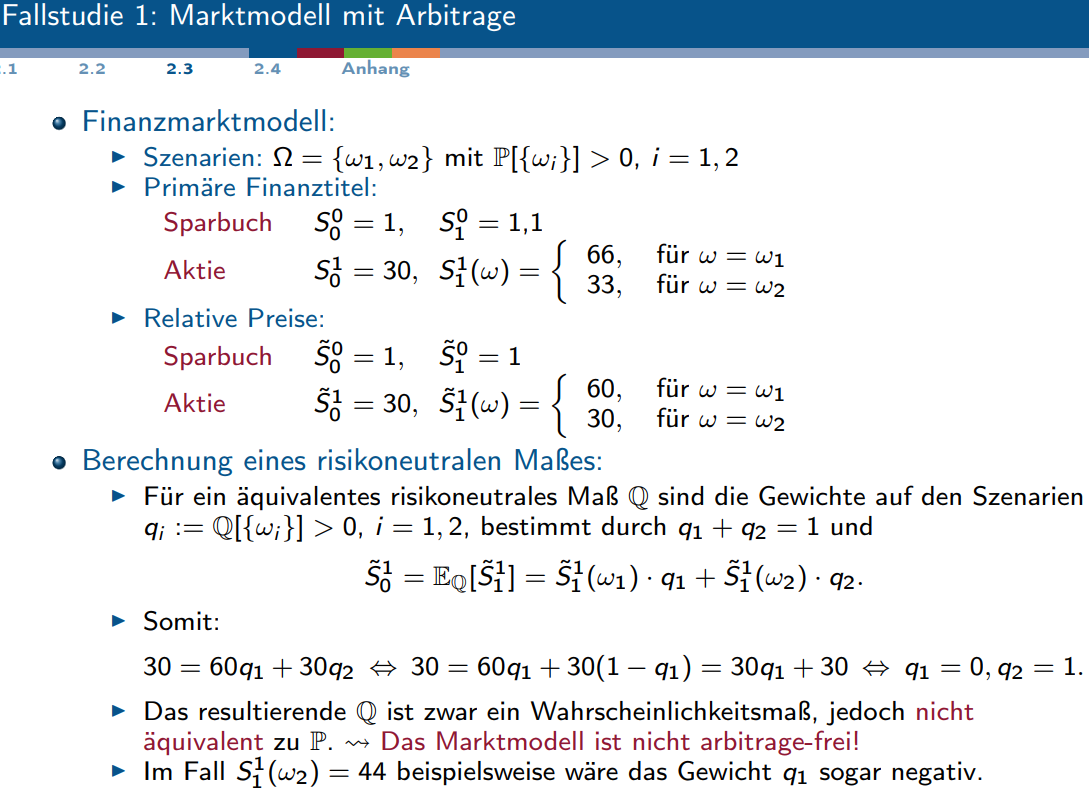
\includegraphics[width=\textwidth]{Bilder/Marktmodell.png}
\end{figure}



\subsubsection{Law of One Price}

\begin{itemize}
\item Es sei $\mathcal{V} := \{V_1^\vartheta | \vartheta \in \mathbb{R}_{d+1}\}$ der lineare Raum aller terminalen Auszahlungen, die durch eine Handelsstrategie 
$\vartheta$ generiert werden können
\item Ein Auszahlung $C_1 \in \mathcal{V}$ wird replizierbar oder auch duplizierbar genannt
\item Eine Handelsstrategie $\vartheta$ mit $C_1 = V_1^\vartheta$ ist i.A. nicht eindeutig; Es gilt jedoch: Law of One Price
\end{itemize}


\subsubsection{Definition Law of One Price}
Falls $C_1 \in \mathcal{V}$ in einem arbitrage-freien Marktmodell die Form $C_1=V_1^\vartheta = V_1^\xi$ $\mathbb{P}$-f.s. für zwei verschiedene Handelsstrategien $\vartheta, \xi \in \mathbb{R}^{d+1}$ besitzt, so gilt $V_0^\vartheta=V_0^\xi$

\begin{itemize}
\item Mit Blick auf das Law of One Price ist es sinnvoll, den Preis von $C_1 \in \mathcal{V}$ zu definieren durch die Kosten der perfekten Replikation: \\
$C_0:= V_0^\vartheta$, falls $C_1=V_1^\vartheta$ \\
Anderenfalls kann Arbitrage generiert werden!
\item Für jedes risikoneutrale Maß $\mathcal{Q} \in \mathbb{Q}$ kann der Preis $C_0$ - und zwar losgelöst von der Berechnung einer replizierenden Strategie - berechnet werden durch
\begin{equation}
C_0= S_0^0E_\mathbb{Q} \left[ \frac{C_1}{S_1^0} \right] = E_\mathbb{Q} \left[ \frac{C_1}{1+r} \right]
\end{equation}
Dies ist die risikoneutrale Bewertungsformel.
\end{itemize}


Die risikoneutrale Bewertungsformel hat zwei Vorteile:\\ 
- Für replizierbare Auszahlungen kann die Bewertung von der Berechnung der
Replikationsstrategie entkoppelt werden. Es genügt, einen Erwartungswert
unter $\mathcal{Q}$ zu berechnen! \\
- Die risikoneutrale Bewertungsformel ist auch zur Bewertung von
nicht-replizierbaren Auszahlungen anwendbar.


\subsection{Risikoneutrale Bewertung von Finanzderivaten }


\subsubsection{Contingent Claim}
Charakterisierung:
\begin{itemize}
\item Contingent Claims sind Verträge zwischen Handelspartnern, die verbindlich
Zahlungen festlegen, die zu zukünftigen Zeitpunkt geleistet werden.
\item Die Höhe der Zahlungen erfolgt in Abhängigkeit von zukünftigen Ereignissen.
\begin{itemize}
\item Finanzderivate: Die Höhe der Zahlungen hängt z. B. von der Kursentwicklung
von Referenzprodukten (Aktien, Anleihen, Währungen, Rohstoffe etc.) ab.
\item Zahlungen aus Versicherungsrisiken: Zahlungen sind durch das Eintreten und
den Umfang von Schäden bestimmt (z. B. CatBonds, Longevity Swaps).
\end{itemize}
\end{itemize}

\subsubsection{Definition Europäischer Contigent Claim}
\begin{itemize}
\item Ein Contingent Claim ist eine Zufallsvariable $C_1$ auf dem zugrunde liegenden
Wahrscheinlichkeitsraum $(\Omega, \mathcal{F}, \mathbb{P})$ mit $0\leq C_1 < \inf$ $\mathcal{P}$-f.s.
\item Ein Contingent Claim heißt Derivat der primären Finanztitel, falls \\
$C_1 = f(S_0^0, S_0^1, ..., S_0^d; S_1^0, S_1^1,..., S_1^d)$
 \end{itemize}


\subsubsection{Definition arbitrage-freie Preise}
Eine reelle Zahl $C_0 \geq 0$ heißt arbitrage-freier Preis eines Contingent Claims
$C_1$, falls das ursprüngliche Marktmodell nach Erweiterung um den Finanztitel $S_0^{d+1}=C_0$ und $S_1^{d+1}=C_1$ arbitrage-frei bleibt. \\
Die Menge aller arbitrage-freien Preise von $C_1$ wird mit $\mathcal{C}_0$ bezeichnet


\begin{figure}[ht]
	\centering
	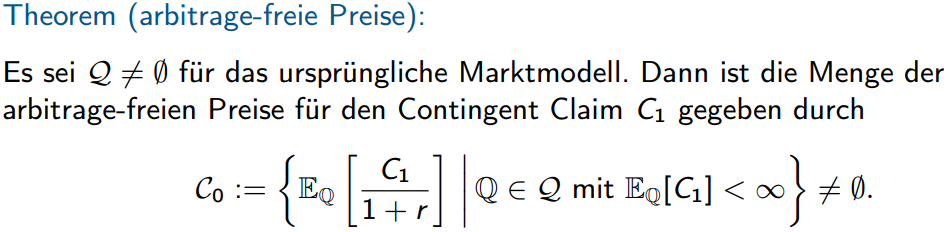
\includegraphics[width=\textwidth]{Bilder/Arbitragefrei.png}
\end{figure}


\subsubsection{Replizierbarer Contingent Claim}
Ein Contigent Claim $C_1$ ist replizierbar, falls $C_1 = V_1^\vartheta$ $\mathcal{P}$-f.s. für ein $\vartheta \in \mathbb{R}^{d+1}$

\subsubsection{Dichotomie für arbitrage-freie Preise} 
Es sei $C_1$ ein Contingent Claim in einem arbitrage-freien Finanzmarktmodell. \\
1. $C_1$ ist replizierbar genau dann, wenn der arbitrage-freie Preis eindeutig ist. In diesem Fall entspricht der Preis den Kosten der perfekten Replikation. \\
2. Ist $C_1$ nicht replizierbar, so gilt $C_0^{inf} < C_0^{sup}$ und die Menge $C_0$ der arbitrage-freien Preise ist das offene Intervall $\mathcal{C}_0=(C_0^{inf}, C_0^{sup})$

\begin{figure}[ht]
	\centering
	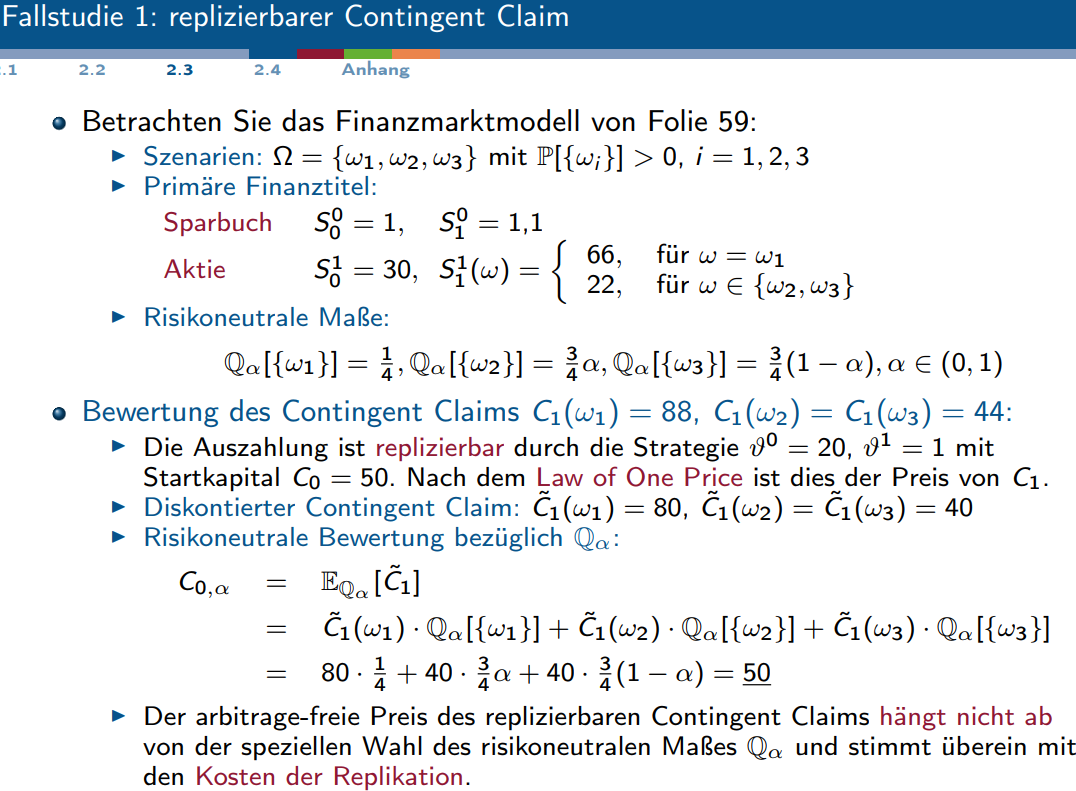
\includegraphics[width=\textwidth]{Bilder/Contingent.png}
\end{figure}



\subsection{Vollständige und unvollständige Finanzmarktmodelle}


\subsubsection{Replizierbare Contingent Claims}
In einem Finanzmarktmodell sind die replizierbaren Contingent Claims die
linearen Portfolios der zugrunde liegenden primären Finanztitel, d. h. es gibt
eine Handelsstrategie $\vartheta \in \mathbb{R}^{d+1}$ mit
\begin{equation}
C_1=\vartheta^0S_1^0 + \vartheta^1S_1^1 + ...+ \vartheta^dS_1^d
\end{equation}
Replizierbare Contingent Claims besitzen einen eindeutigen arbitrage-freien
Preis, gegeben durch die Kosten der perfekten Replikation


\subsubsection{Definition Vollständige und unvollständige Finanzmarktmodelle}
Ein arbitrage-freies Marktmodell heißt vollständig, falls jeder Contingent Claim
replizierbar ist. Anderenfalls heißt das arbitrage-freie Marktmodell unvollständig.

\subsubsection{Theorem 2. Funamentalsatz der Wertpapierbewertung}
Ein arbitrage-freies Finanzmarktmodell ist vollständig genau dann, wenn es genau
ein äquivalentes risikoneutrales Maß gibt, d. h. $|\mathcal{Q}| =1$




\section{Risikoneutrale Bewertung in Mehrperiodenmodellen}


\subsection{Grundbegriffe und -prinzipien in Mehrperiodenmodellen }

\subsubsection{Zeitdiskrete vs. zeitstetige Modellierung (Mehrperiodenmodelle}

\begin{itemize}
\item Finanzmarktmodell in diskreter Zeit: nur abzählbar viele Handelszeitpunkte
\item Die Modellierung kann aber auch in stetiger Zeit erfolgen: Die Modellierung von Preisprozessen primärer Finanzprodukte erfolgt durch
Stochastische Differentialgleichungen. Finanzmathematik in stetiger Zeit basiert auf den Methoden der Stochastischen Analysis
\end{itemize}

\subsubsection{Zeitdiskrete Mehrperiodenmodelle - Handelsstrategie}
\begin{itemize}
\item Die Anzahl von Finanzprodukt $i$, die in der Periode $(t - 1; t]$ im Portfolio
gehalten wird, wird mit $\vartheta_t^i$ bezeichnet.
\begin{itemize}
\item Die Stückzahl $\vartheta_t^i$ wird zu Beginn der Handelsperiode auf Basis der verfügbaren Information $\mathcal{F}_{t-1}$ durch eine*n Investor*in festgelegt.
\item Damit ist diese Stückzahl bis $t - 1$ nicht bekannt, also eine Zufallsvariable, und $\mathcal{F}_{t-1}$-messbar.
\end{itemize}
\item  Eine Handelsstrategie ist ein vorhersehbarer stochastischer Prozess mit
Werten in $\mathbb{R}^{d+1}$: $\vartheta=(\vartheta_t)_{t=1,...,T} = ((\vartheta_t^0,...,\vartheta_t^d)^\perp)_{t=1,...,T}$
\end{itemize}

\begin{figure}[ht]
	\centering
	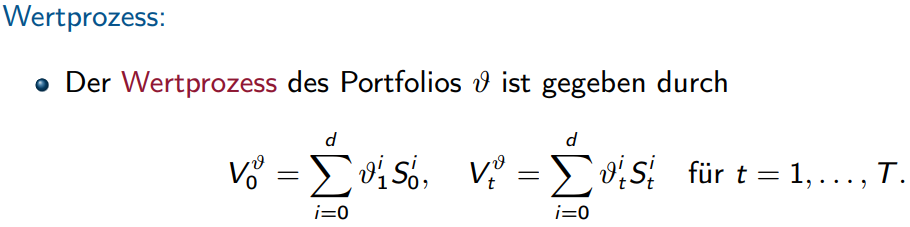
\includegraphics[width=0.8 \textwidth]{Bilder/Wertprozess.png}
\end{figure}

\begin{figure}[ht]
	\centering
	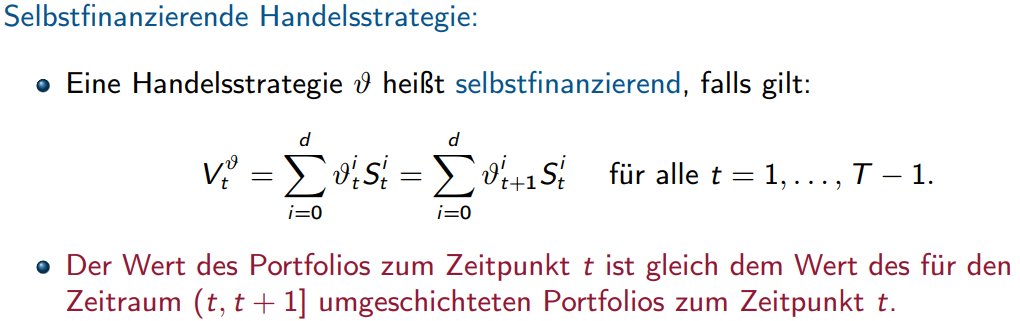
\includegraphics[width=0.8 \textwidth]{Bilder/Handelsstrategie.png}
\end{figure}


\subsubsection{Bewertung von Contingent Claims}
Ziel: Bewertung einer bedingten Auszahlung $C_T$ mit Fälligkeit in $T$.
\begin{itemize}
\item Replizierendes Portfolio: selbstfinanzierende Strategie $\vartheta$ mit $V_T^\vartheta (\omega) = C_T(\omega)$. Diese Gleichung muss in allen Szenarien $\omega \in \Omega$ gelten
\item Vollständiges Finanzmarktmodell:
Jeder Contingent Claim ist replizierbar.
\item Unvollständiges Finanzmarktmodell:
Der Markt ist nicht vollständig, d. h. es gibt Contingent Claims, die nicht
replizierbar sind
\item Ist der Contingent Claim CT replizierbar, so muss der Preis gleich den Kosten
der perfekten Replikation sein. Anderenfalls gibt es Arbitrage!

\end{itemize}

\begin{figure}[ht]
	\centering
	\includegraphics[width=0.8 \textwidth]{Bilder/Martingalmaß.png}
\end{figure}

\begin{itemize}
\item 1. Fundamentalsatz: $\exists$ äquivalentes Martingalmaß $\Leftrightarrow$ Markt arbitrage-frei
\item 2. Fundamentalsatz: $\exists$! äquivalentes Martingalmaß $\Leftrightarrow$ Markt vollständig
\end{itemize}






%----------------------------------------------------------------------

%KAPITEL 3

%----------------------------------------------------------------------

\section{Grundlagen der Zinstheorie}

\subsection{Arten der Versinsung}

\begin{itemize}
	\item Konversionsperiode: Zeitintervall an dessen Ende die Zinsen gutgeschrieben werden (meist 1 Jahr)
	\item $p$: Zinsfu{\ss} f\"ur eine Zeiteinheit
	\item $r=\frac{p}{100}$ Zinssatz
	\item diskontierliche Zinsgutschrift: Gutschrift am Ende einer Periode
		\begin{itemize}
			\item einfache Verzinsung: $K_t = K_0(1+[t]r)$
			\item Zusammengesetzte Verzinsung: $K_t=K_0(1+r)^{[t]}$
		\end{itemize}
	\item kontinuierliche Zinsgutschrift
		\begin{itemize}
			\item einfache Verzinsung: $K_t = K_0(1+tr)$
			\item Zusammengesetzte Verzinsung: $K_t=K_0(1+r)^{t}$
		\end{itemize}
	\item Gemischte Verzinsung: $K_t=K_0(1+r)^{[t]}(1+(t-[t])r)$ f\"ur ganze Jahre $[t]$ und unterj\"ahrigen Teil $t-[t]$
\end{itemize}

\subsection{Barwerte und Endwerte}

\begin{itemize}
	\item Vollkommener Kapitalmarkt in diskreter Zeit:
	\begin{itemize}
		\item zu einem deterministischen Periodenzinssatz $r>0$ k\"onnen beliebig hohe Geltbetr\"age angelegt und beliebig hohe Kredite aufgenommen werden
		\item Beliebige Zahlungen zu einem beliebigen Zeitpunkt k\"onnen auf einen beliebigen anderen Zeitpunkt zu Kapitalmarktbedingungen transferiert werden.
	\end{itemize}
	\item Kapitalmarktbewertung (Barwert der Zahlungsreihe): \\ $BW_0(r) = \sum_{t=0}^T Z_t q^{-t} = \sum_{t=0}^T Z_tv^t$
	\item Endwert (resultierende Gr\"o{\ss}e als Endwert der Zahlungsreihe): \\ $EW_T(t) = BW_0(r)\cdot q^T = \sum_{t=0}^T Z_t q^{T-t}$
\end{itemize}

\subsection{Allgemeine Zinsstrukturkurven}

\begin{itemize}
	\item Nullkuponanleihe
	\begin{itemize}
		\item liefert normierte Auszahlung 1 zur Maturit\"at $T$
		\item $P(t,T)$ sei der Wert dieser Auszahlung in $t \leq T$, $P(T,T)=1$
		\item $P(t,T)$ vor $t$ nicht mit Sicherheit bekannt, $t \rightarrow P(t,T)$ ist stochastisch
		\item $P(t,T)$ dient als Diskontierungsfaktor, $T \rightarrow P(t,T)$ ist die Diskontkurve in $t$
		\item Nichtnegative Zinsen: Bondpreise $t \rightarrow P(t,T) \leq 1$ mit der Zeit fallend
	\end{itemize}
	\item Spot Rate zum Zeitpunkt $t$: Zins in $t$, der f\"ur eine Anlage von $t$ bis $T$ gezahlt wird
	\item Forward Rate zum Zeitpunkt $t$: Zins, der in $t$ f\"ur eine Anlage von $T$ bis $S \ (t \leq T \leq S)$ vereinbart wird
	\item Arbitragefreiheit: Ein Kapitalbetrag, der in $t$ bis $T$ zur Spot Rate angelegt wird, muss zur Zeit $T$ einen identischen Endwert aufweisen wie der Kapitalbetrag, der revolvierend jeweils \"uber 1 Jahr zu den in $t$ g\"ultigen Forward Rates angelegt wird.
	\item Short Rate zum Zeitpunkt $t$: Zins f\"ur kurzfristige Anlage $r = f_t(t) = lim_{T \downarrow t} r_t^s(T)$
\end{itemize}

\begin{figure}[H]
\centering
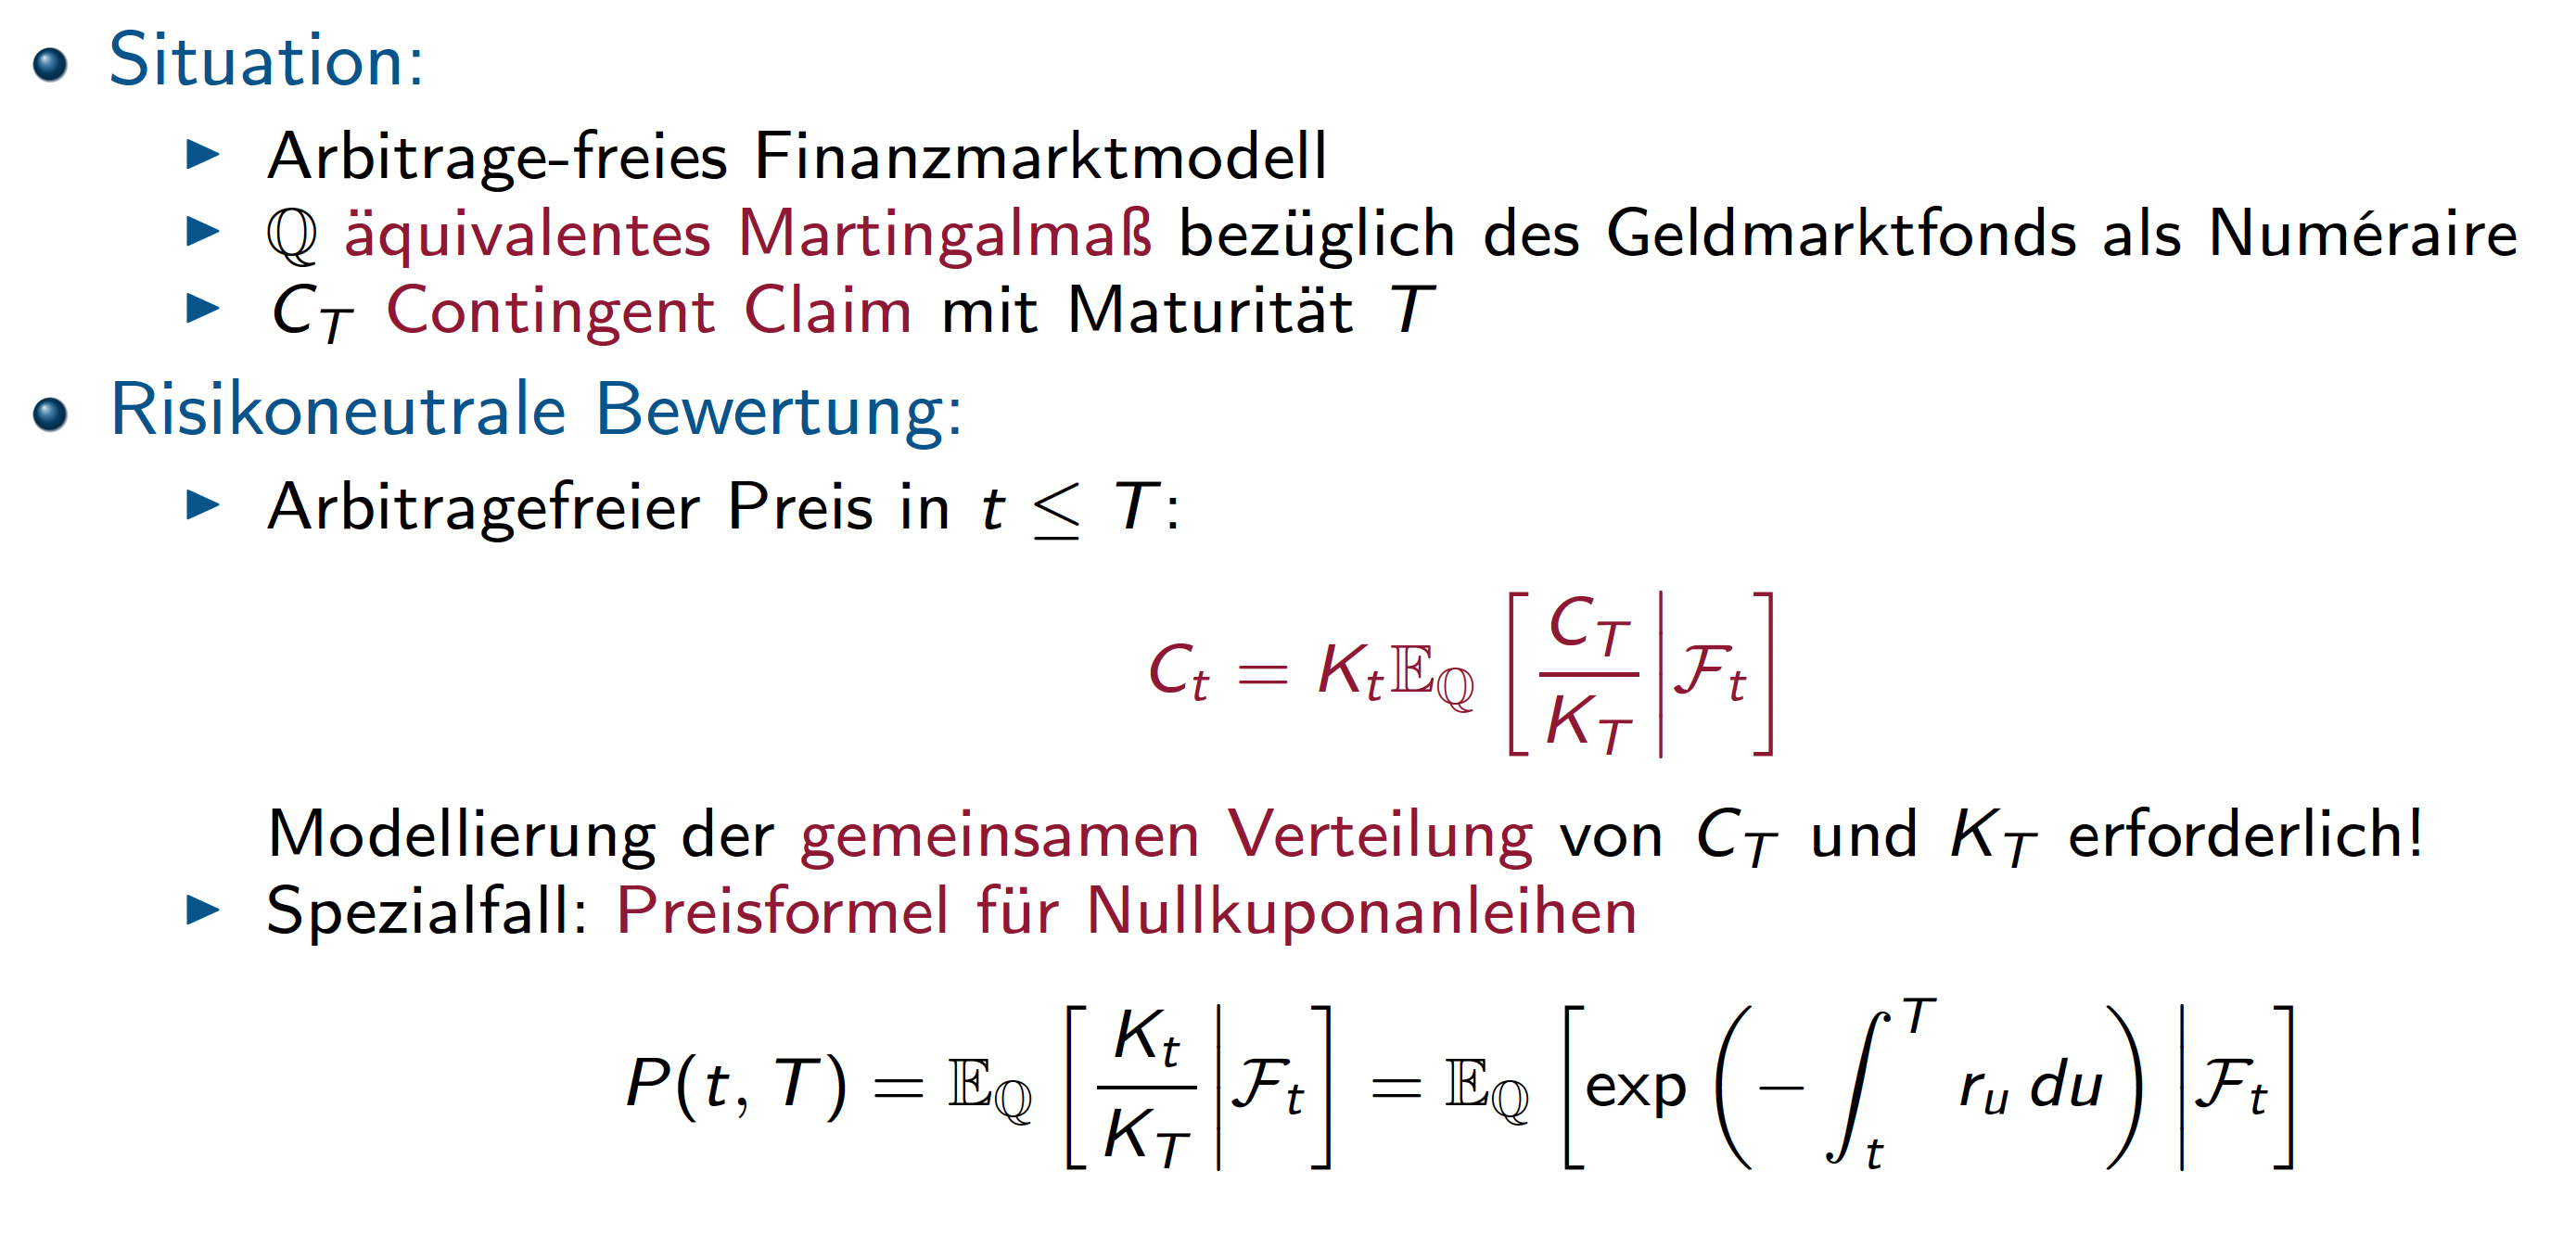
\includegraphics[width=\textwidth]{Bilder/RisikoneutraleBewertung.png}
\end{figure}

\begin{figure}[H]
\centering
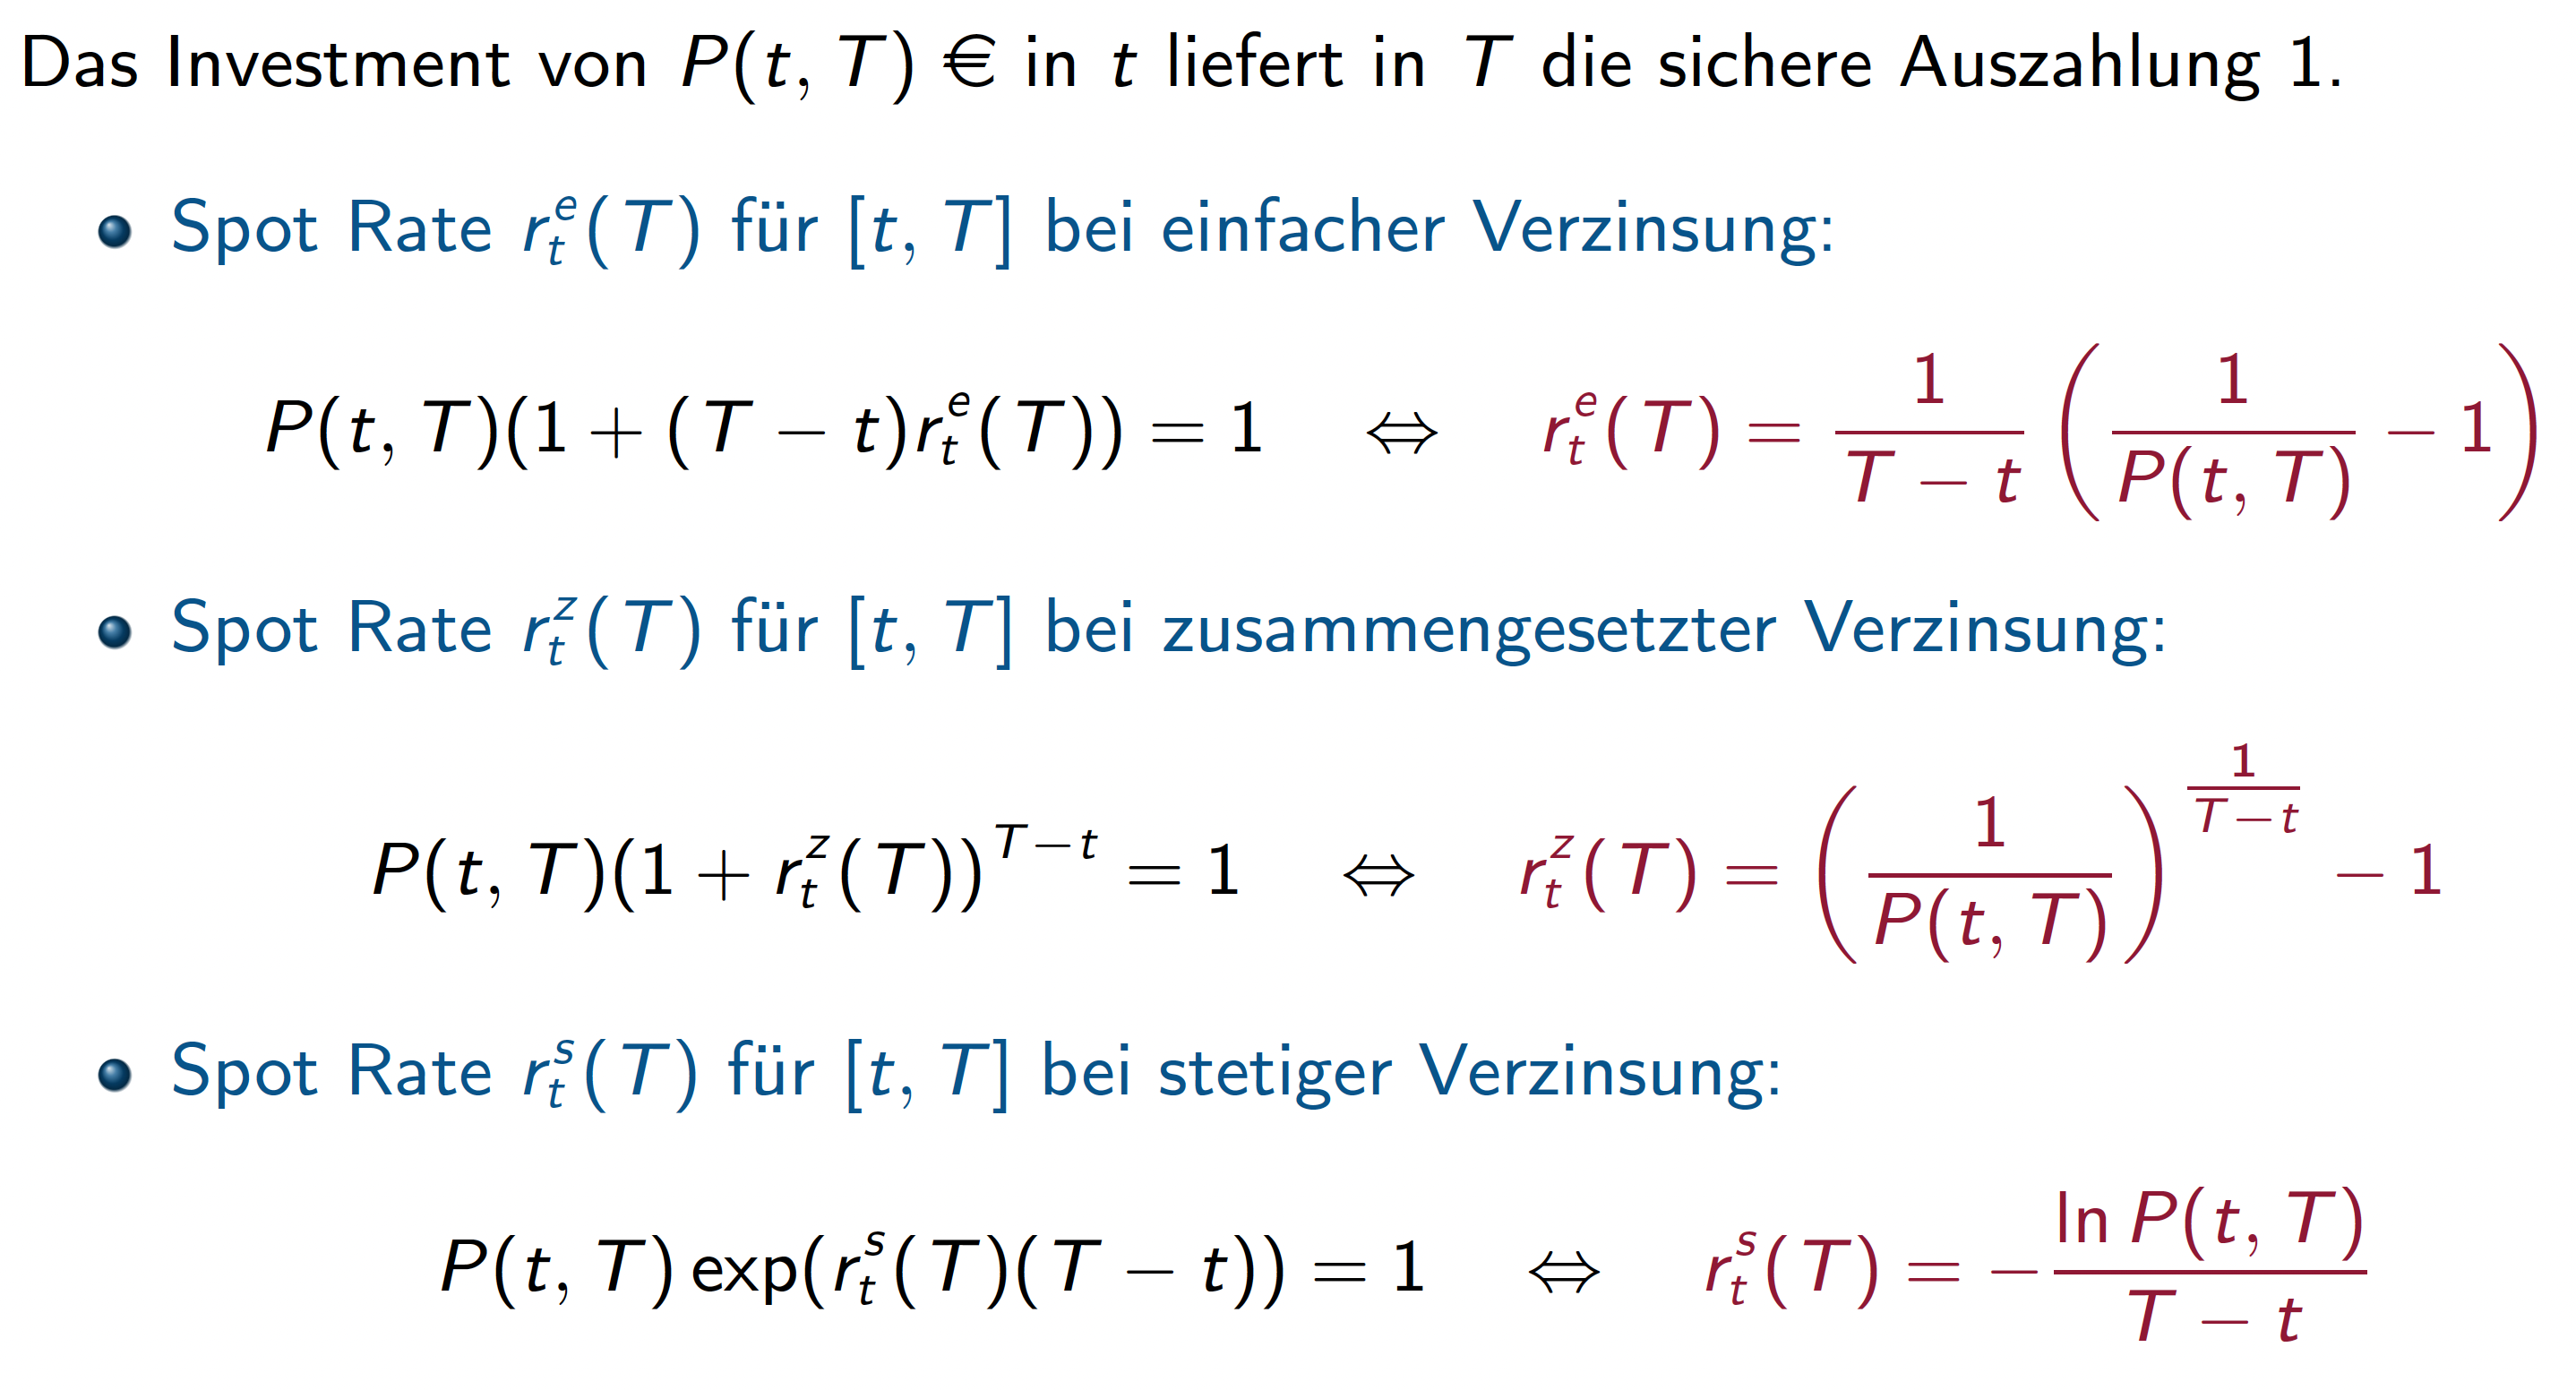
\includegraphics[width=\textwidth]{Bilder/SpotRate.png}
\end{figure}

\begin{figure}[H]
\centering
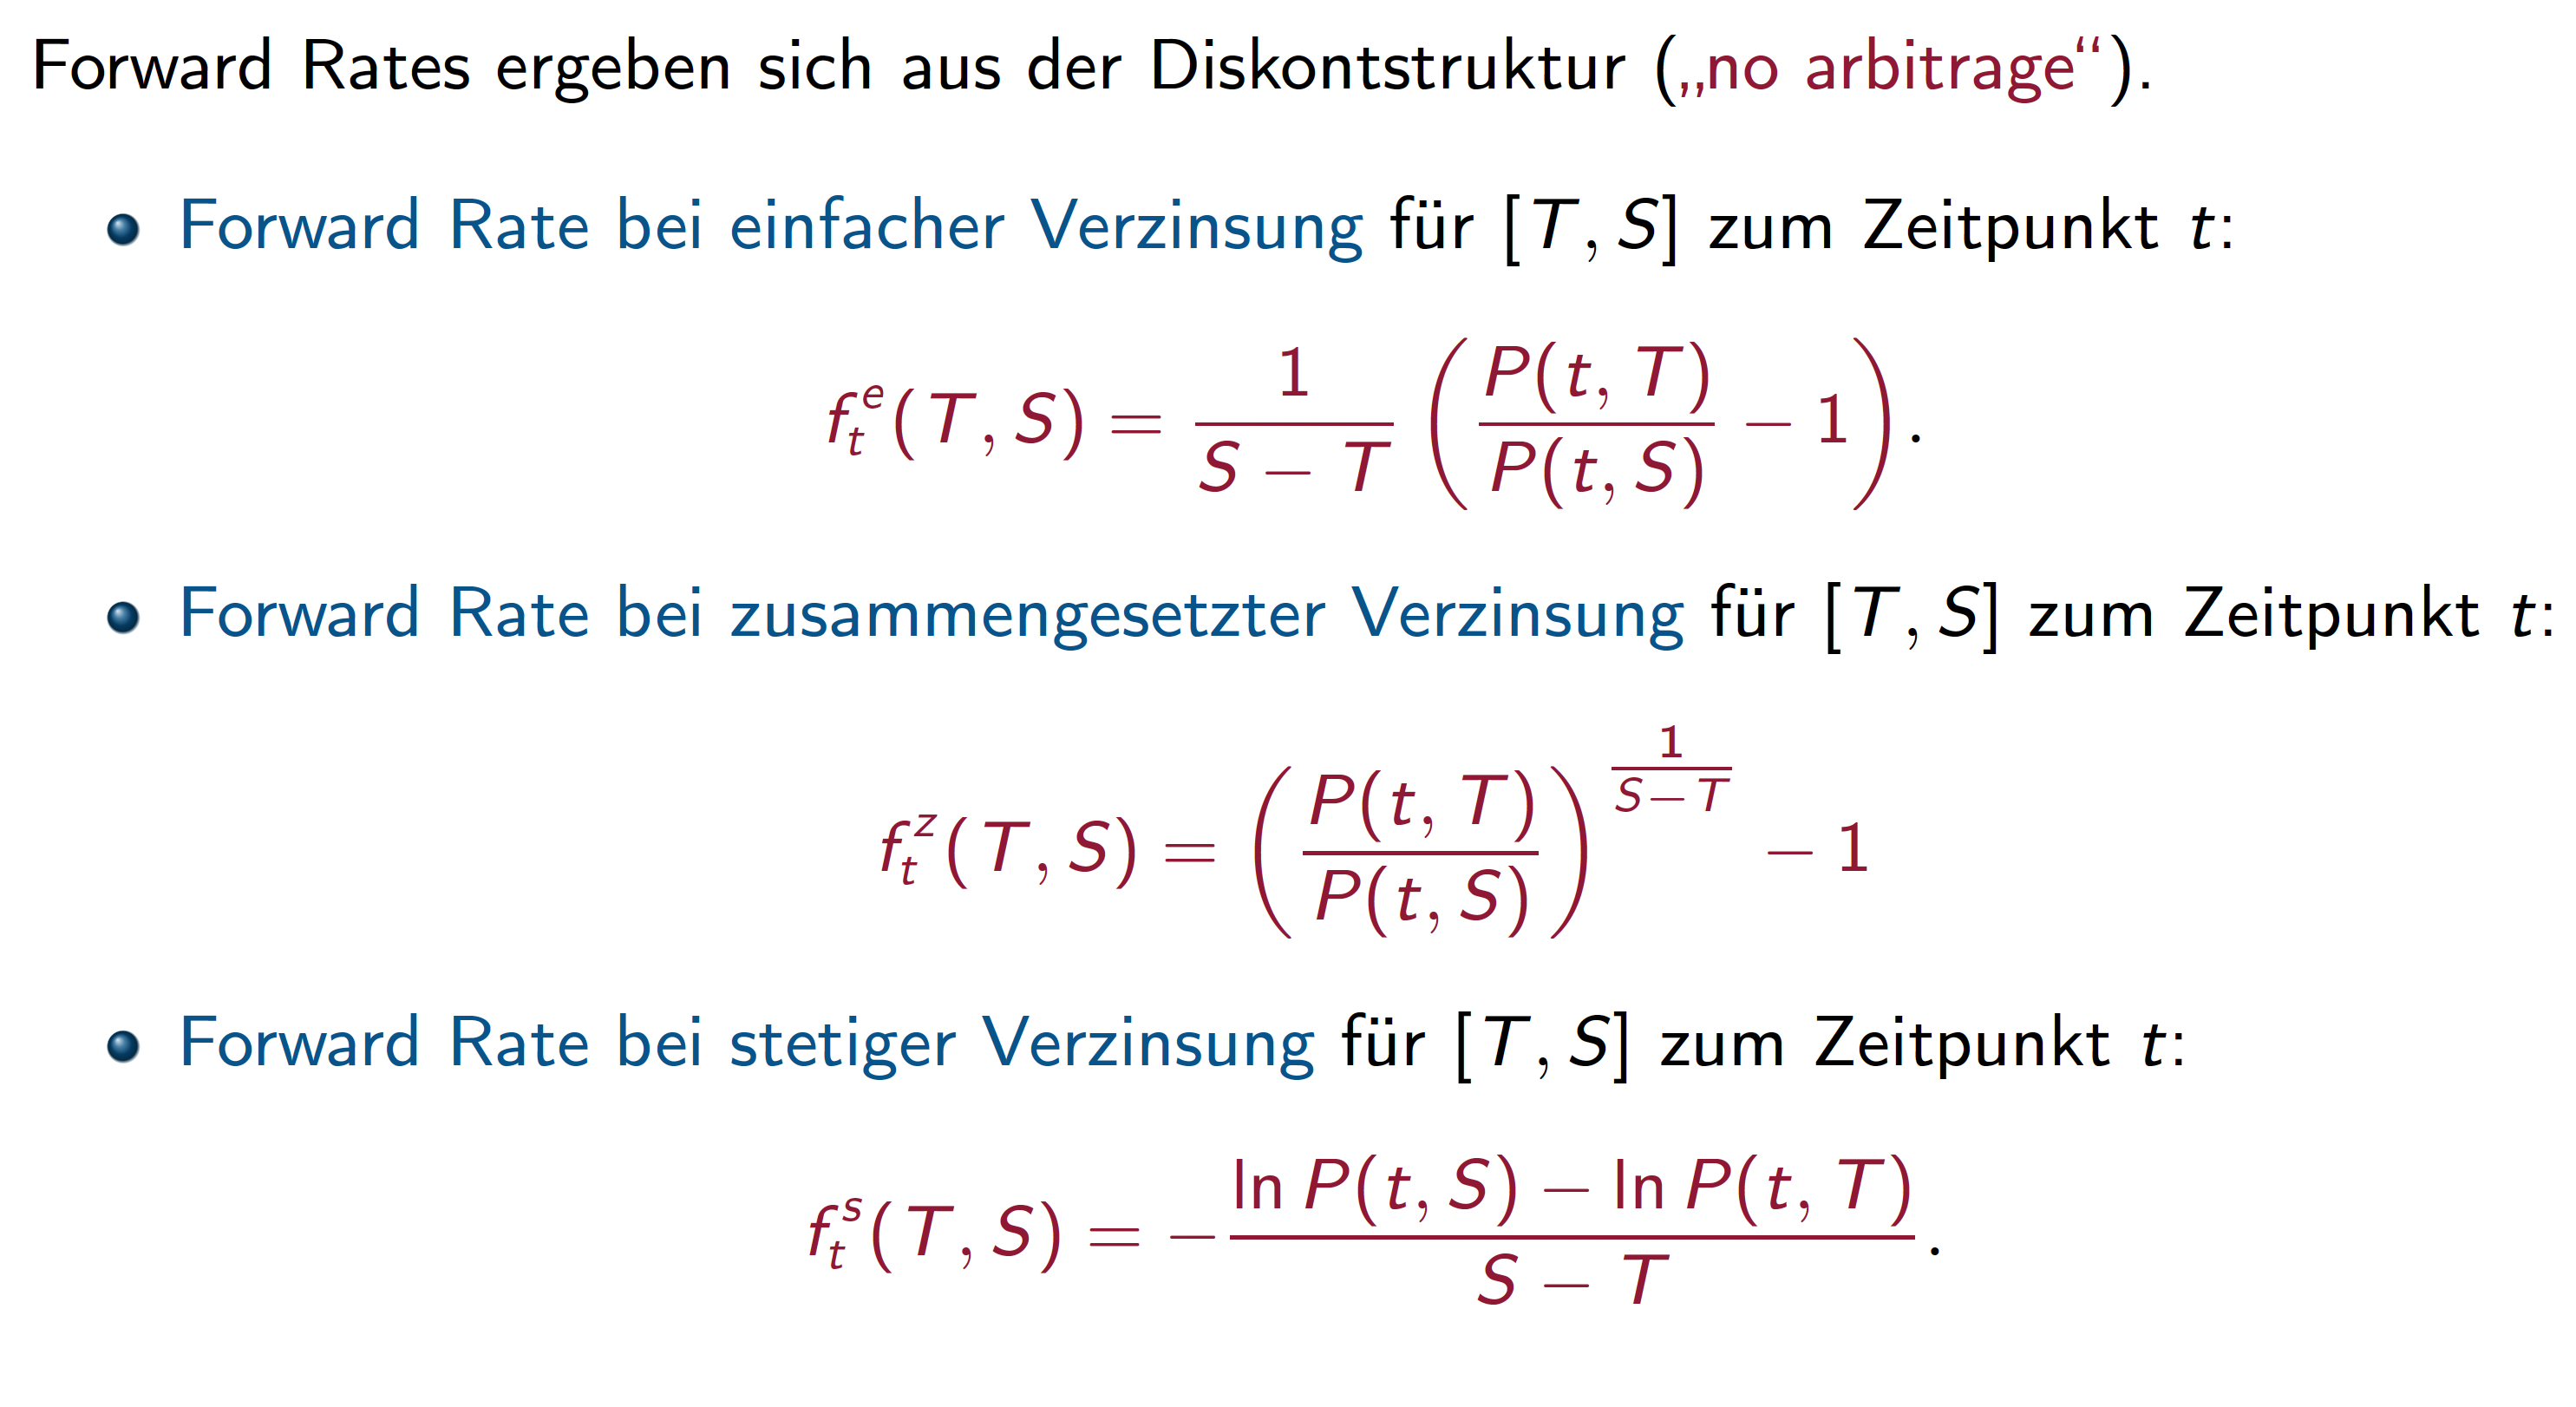
\includegraphics[width=\textwidth]{Bilder/FwdRate.png}
\end{figure}



\section{Zinsprodukte}

\subsection{Einfache Zinsprodukte}

\begin{itemize}
	\item Festverzinsliche Anleihe ist ein Finanztitel mit
	\begin{itemize}
		\item zuk\"unftigen \"aquidistanten Zahlungszeitpunkten $T_1 < T_2 < ...< T_n$
		\item $T_n$ Maturit\"at
		\item deterministischen bei Vertragsabschluss festgelegten Kuponzahlungen $c_1,...,c_n$
		\item einem Nennwert $N$
	\end{itemize}
	\item Variable verzinsliche Anleihen (Floating Rate Notes, Floater)
	\begin{itemize}
		\item mehrere Zinsperioden, nach jeder Periode werden die Zinsen bezahlt
		\item Zinssatz orientiert sich an einem Referenzzinssatz
		\item Zins kann um einen festen Spread \"uber oder unter diesen S\"atzen liegen
		\item Floor Floater: variable verzinsliche Anleihe, die Mindestmarke f\"ur Verzinsung garantiert
		\item Cap Floater: variable verzinsliche Anleihe mit H\"ochstmarke f\"ur Verzinsung
		\item Collared Floater: begrenzen Verzinsung durch Mindest- und H\"ochstssa\"atze
		\item Reverse Floater: Zinszahlung als Differenz zwischen festem Zinssatz und Referenzzinssatz
		\item Floater sind mit anderen Anleihetypen kombinierbar
	\end{itemize}
\end{itemize}


\begin{figure}[H]
\centering
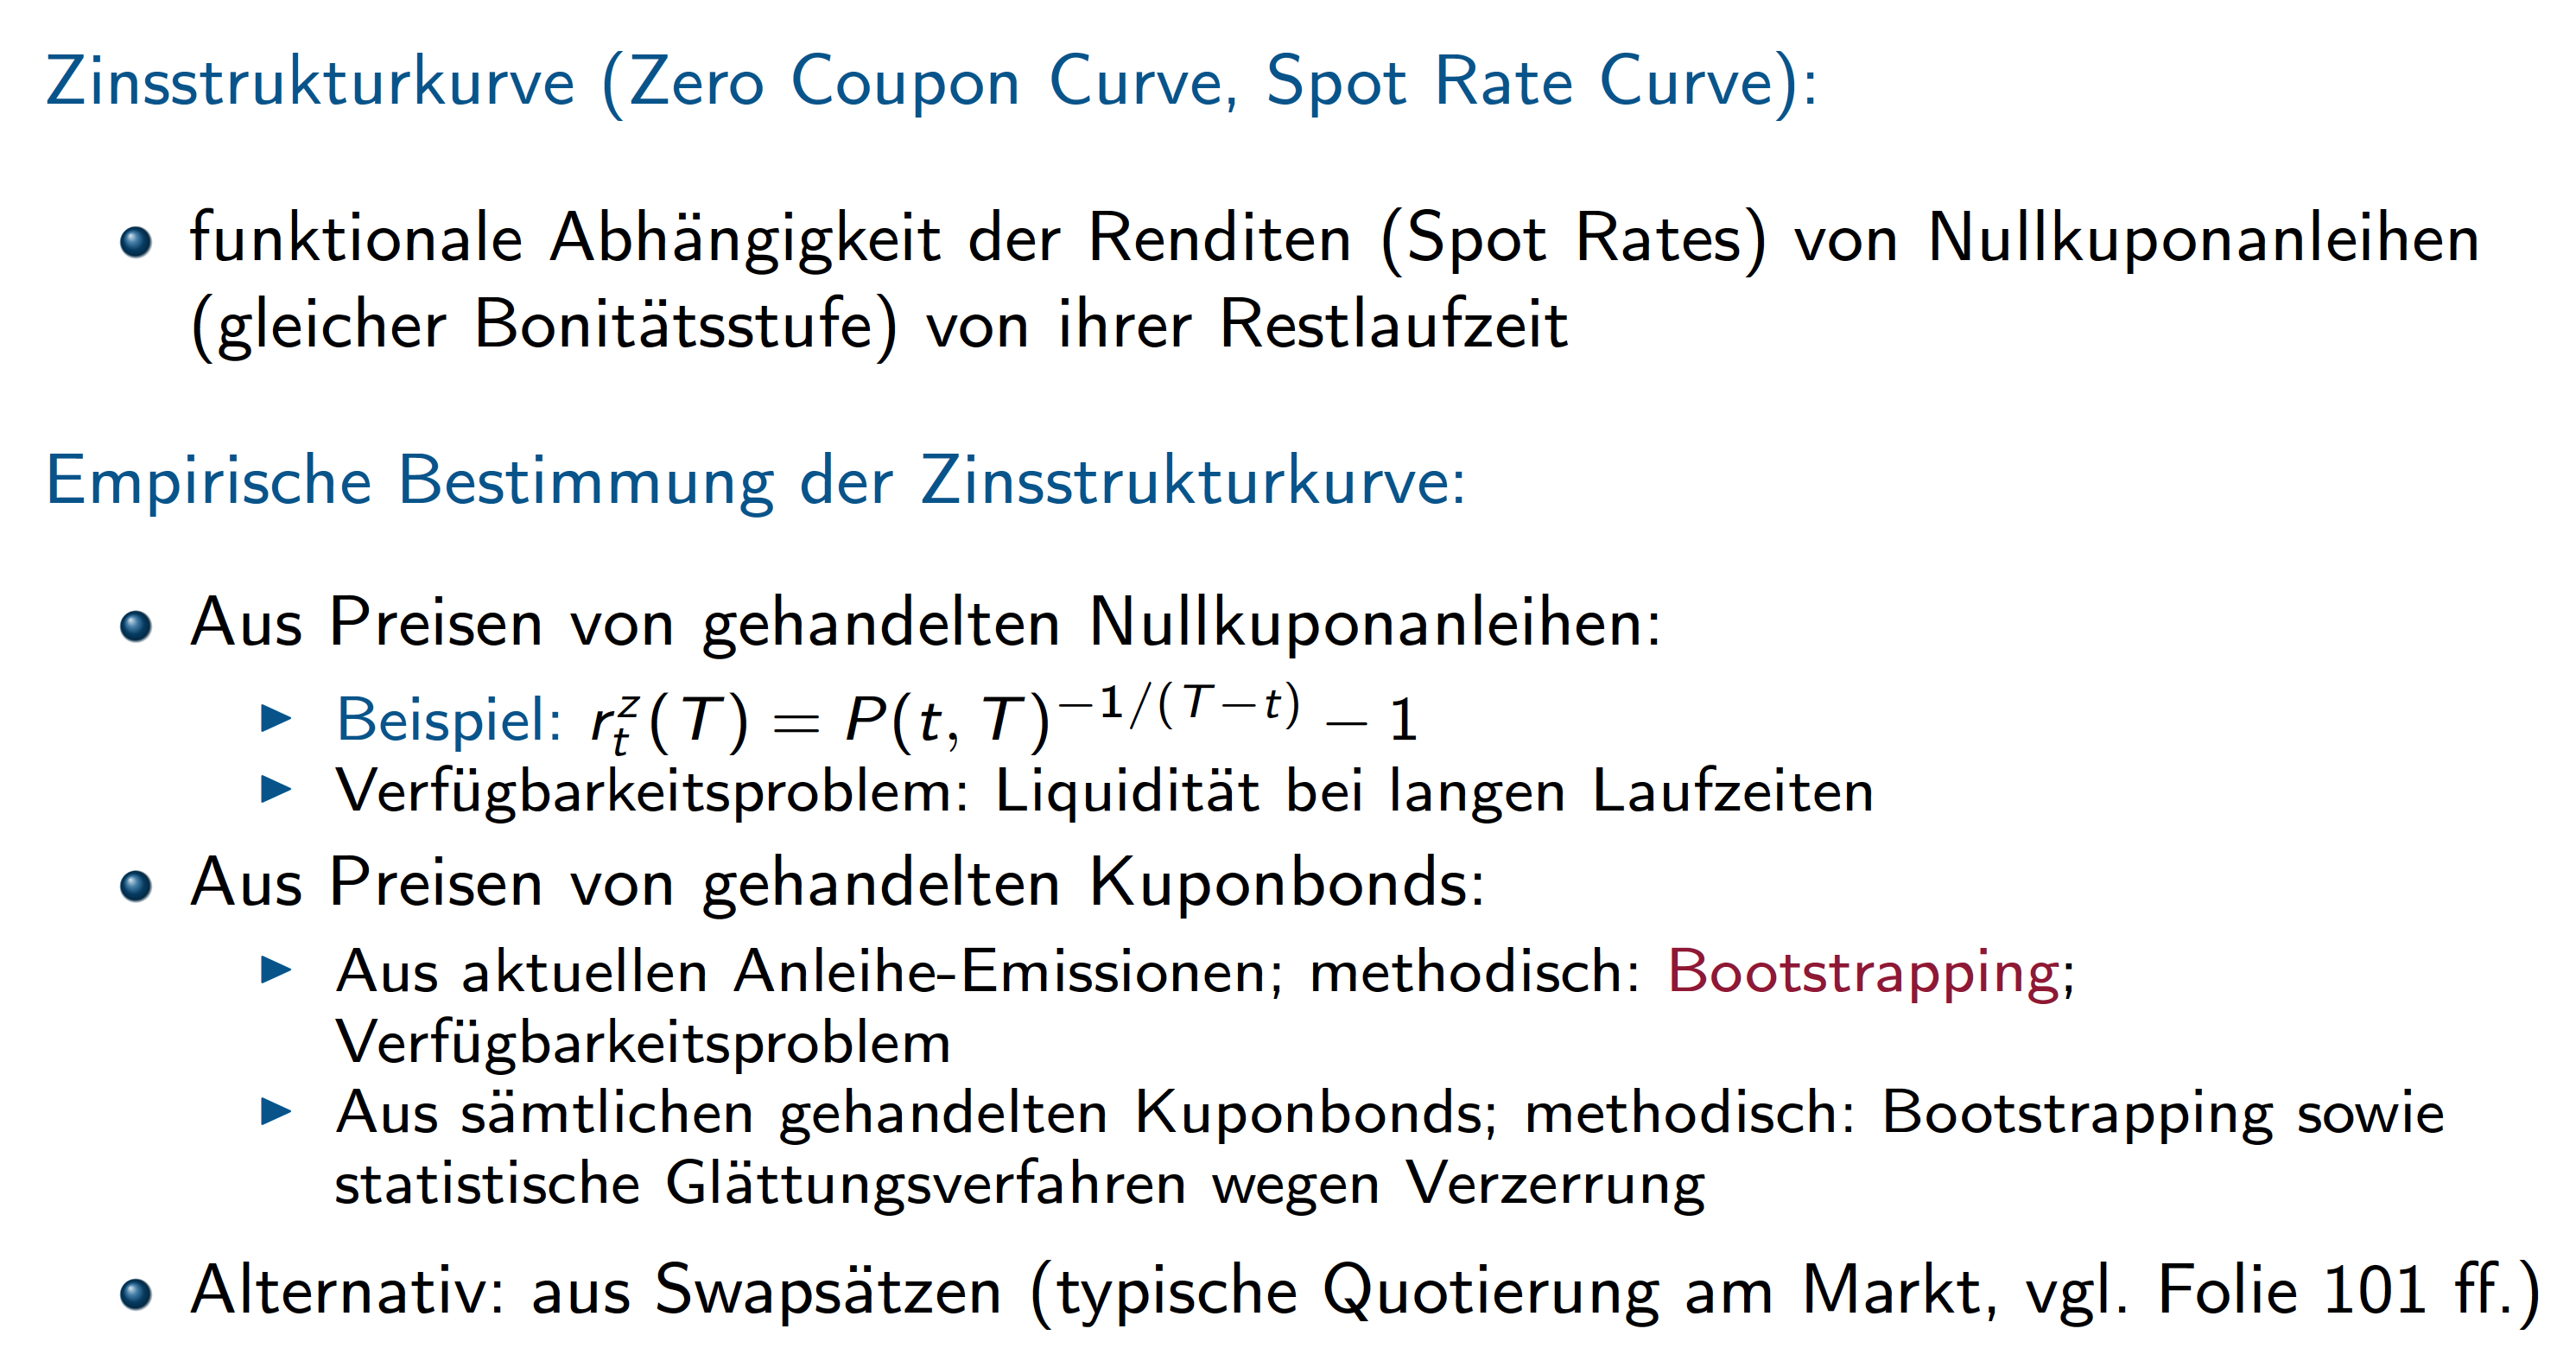
\includegraphics[width=\textwidth]{Bilder/Zinsstrukturkurve.png}
\end{figure}

\subsection{Analyse des Zins\"anderungsrisikos: Duration und Konvexit\"at}

\subsubsection{Annahmen}

\begin{itemize}
	\item Zinsstruktur in $t=0$ flach: $r_0^z (s) = r$ f\"ur alle $s \geq 0$
	\item Zins\"anderung durch einmaligen \"Ubergang in flache Zinsstruktur der H\"ohe $r + \Delta r$
	\item Auswirkungen der Zins\"anderung:
	\begin{itemize}
		\item $\Delta P = P(r + \Delta r) -P(r)$
		\item $\Delta K_T = K_T(r + \Delta r) - K_T(r)$
		\item Steigender Marktzins: Barwert f\"allt, Endwert steigt
		\item Fallender Marktzins: Barwert steigt, Endwert f\"allt
	\end{itemize}
\end{itemize}

\subsubsection{Duration}

\begin{itemize}
	\item Absolute Duration: $DUR^A(r):= -P'(r) = \frac{1}{1+r} \sum_{t=1}^T t Z_t(1+r)^{-t}$
	\item Absolute Duration ist ein approximatives Ma{\ss} f\"ur die Kurs\"anderung bei absoluter Zins\"anderung: $\Delta P(r) \approx -DUR^A(r) \cdot \Delta r$
	\item Absolute Duration mit Konvexit\"at: $\Delta P(r) \approx -DUR^A(r) \cdot \Delta r + \frac{1}{2} CONV^A(r) \cdot (\Delta r)^2$
	\item $CONV^A(r) = P''(r)$
	\item Erste Ableitung der Barwertfunktion mit negativem Vorzeichen
	\item Zins\"anderungsrisiko ist gr\"o{\ss}er, wenn Duration gr\"o{\ss}er
	\item Modifizierte Duration: $DUR^M(r) := \frac{DUR^A}{P(r)} = \frac{P'(r)}{P(r)} = (\frac{1}{1+r}  \sum_{t=1}^T tZ_t(1+r)^{-t}) / P(r)$
	\item Modifizierte Duration ist ein approximatives Ma{\ss} f\"ur die relative Kurs\"anderung bei absoluter Zins\"anderung: $\frac{\Delta P(r)}{P(r)} \approx -DUR^M(r) \cdot \Delta r$
	\item Modifizierte (Relative) Konvexit\"at: $\frac{\Delta P(r)}{P(r)} \approx -DUR^M(r) \cdot \Delta r + \frac{1}{2} CONV(r) \cdot (\Delta r)^2$
	\item $CONV(r) = \frac{P''(r)}{P(r)}$
	\item Duration von 3 Faktoren beeinflusst:
	\begin{itemize}
		\item Laufzeit der Bonds
		\item H\"ohe des Kupons
		\item Marktzins
	\end{itemize}
	\item d.h.:
	\begin{itemize}
		\item Duration sinkt, wenn Kupon steigt
		\item Duration sinkt, wenn Marktzins steigt
		\item Je l\"anger die Laufzeit, desto gr\"o{\ss}er die Duration
	\end{itemize}
\end{itemize}

\subsection{Komplexere Zinsprodukte}

\subsubsection{Forward-Kontrakt}

\begin{figure}[H]
\centering
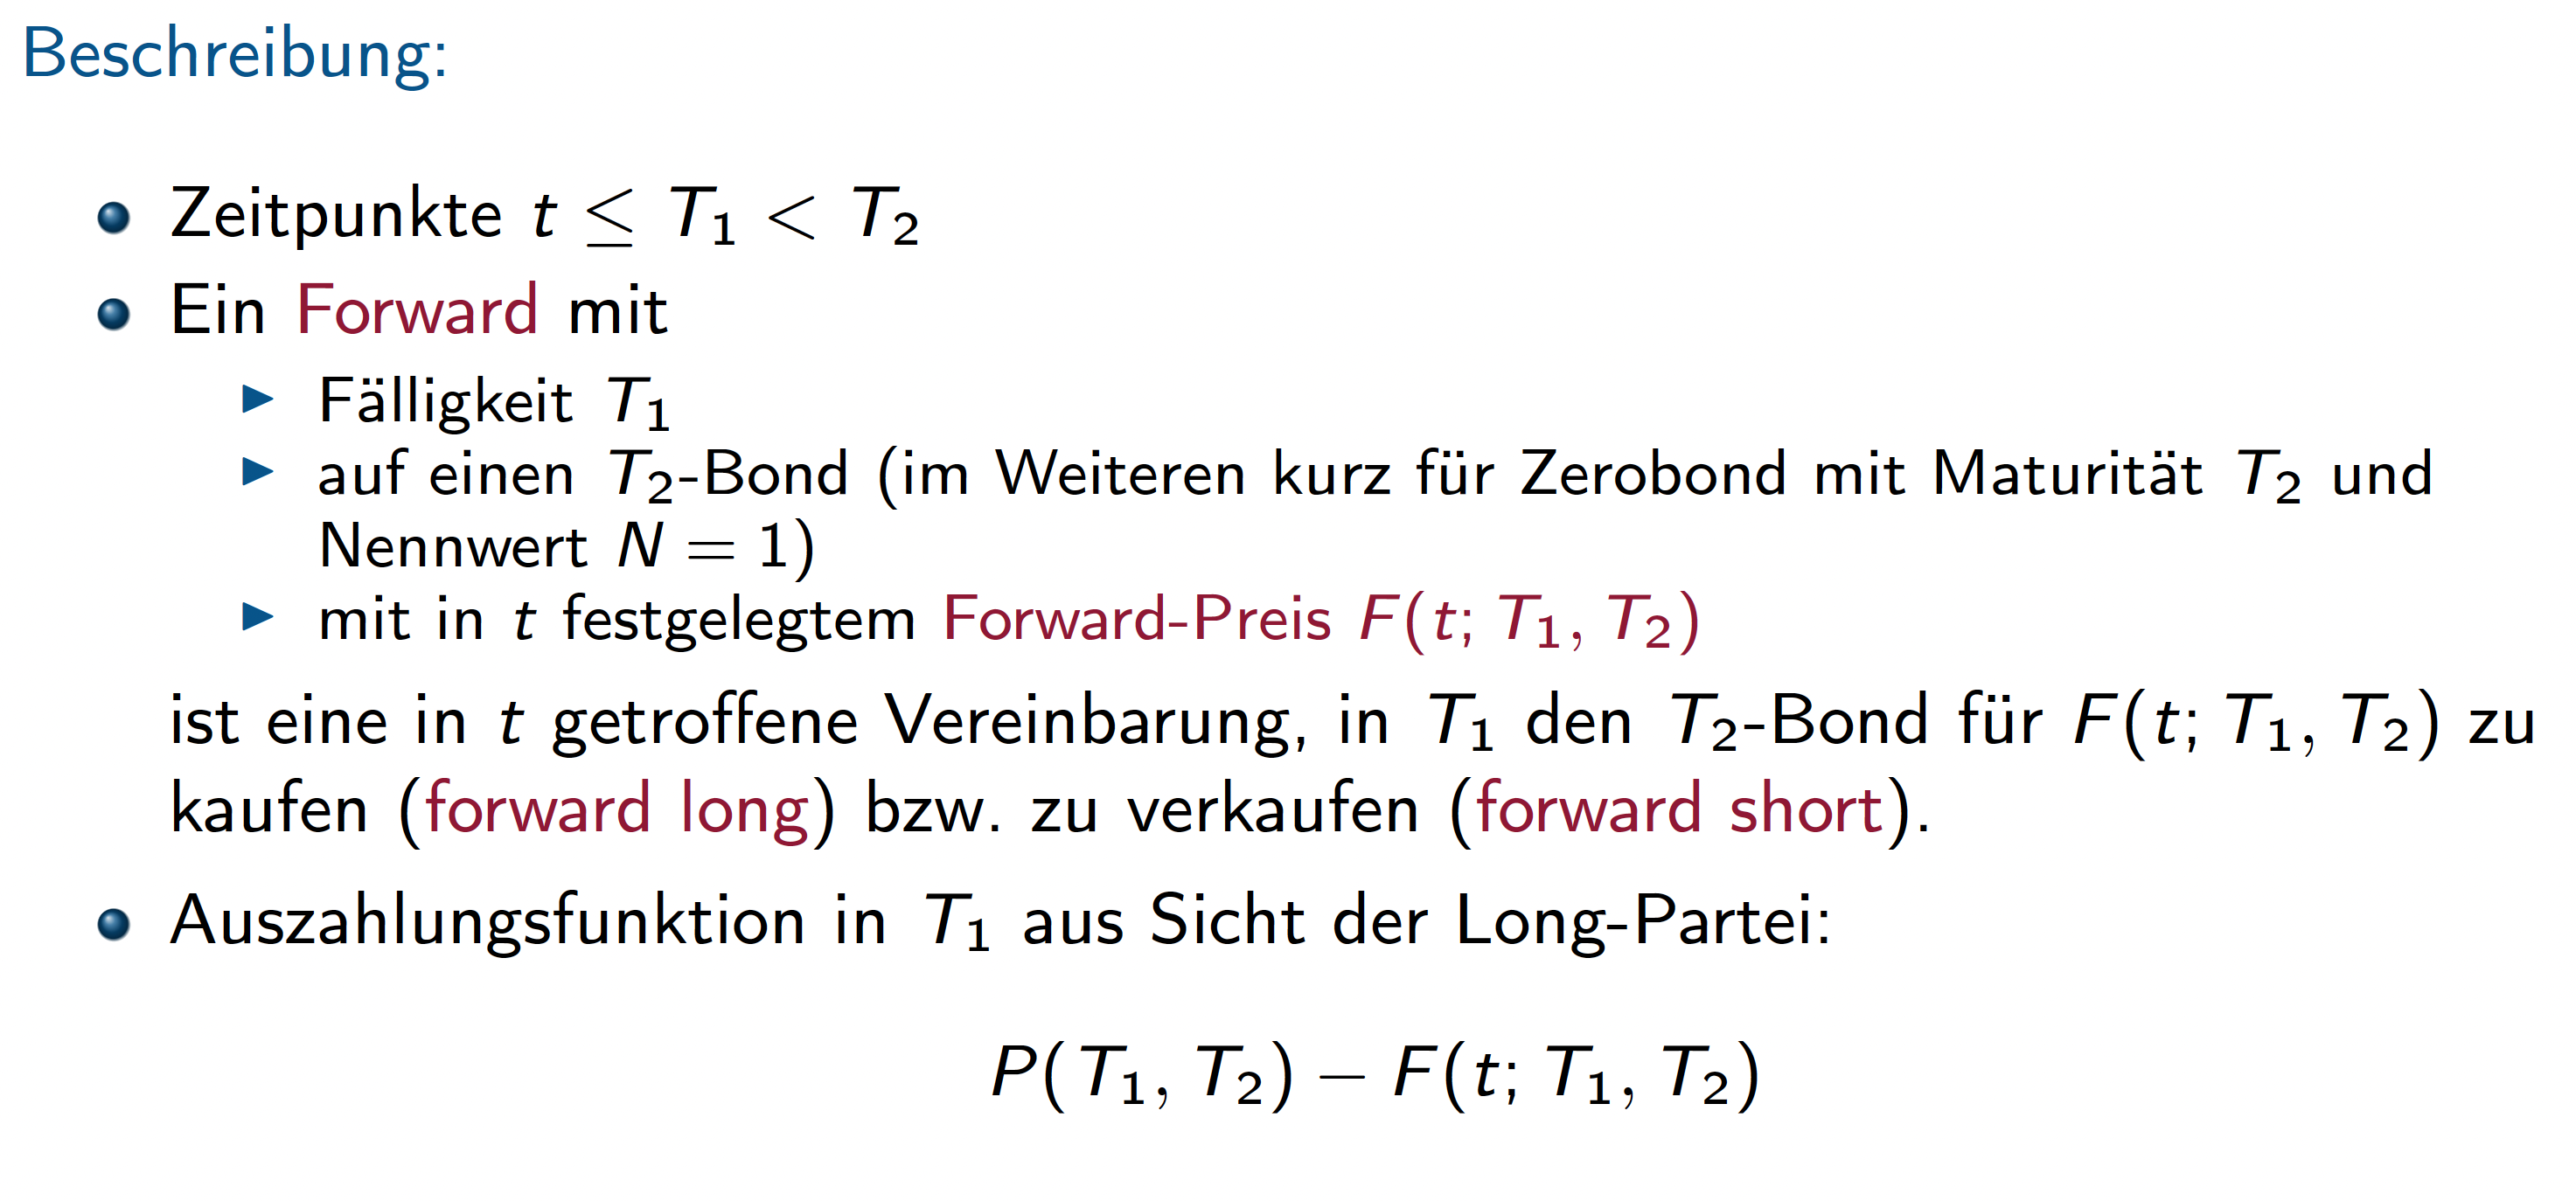
\includegraphics[width=\textwidth]{Bilder/FwdKontrakt1.png}
\end{figure}

\begin{figure}[H]
\centering
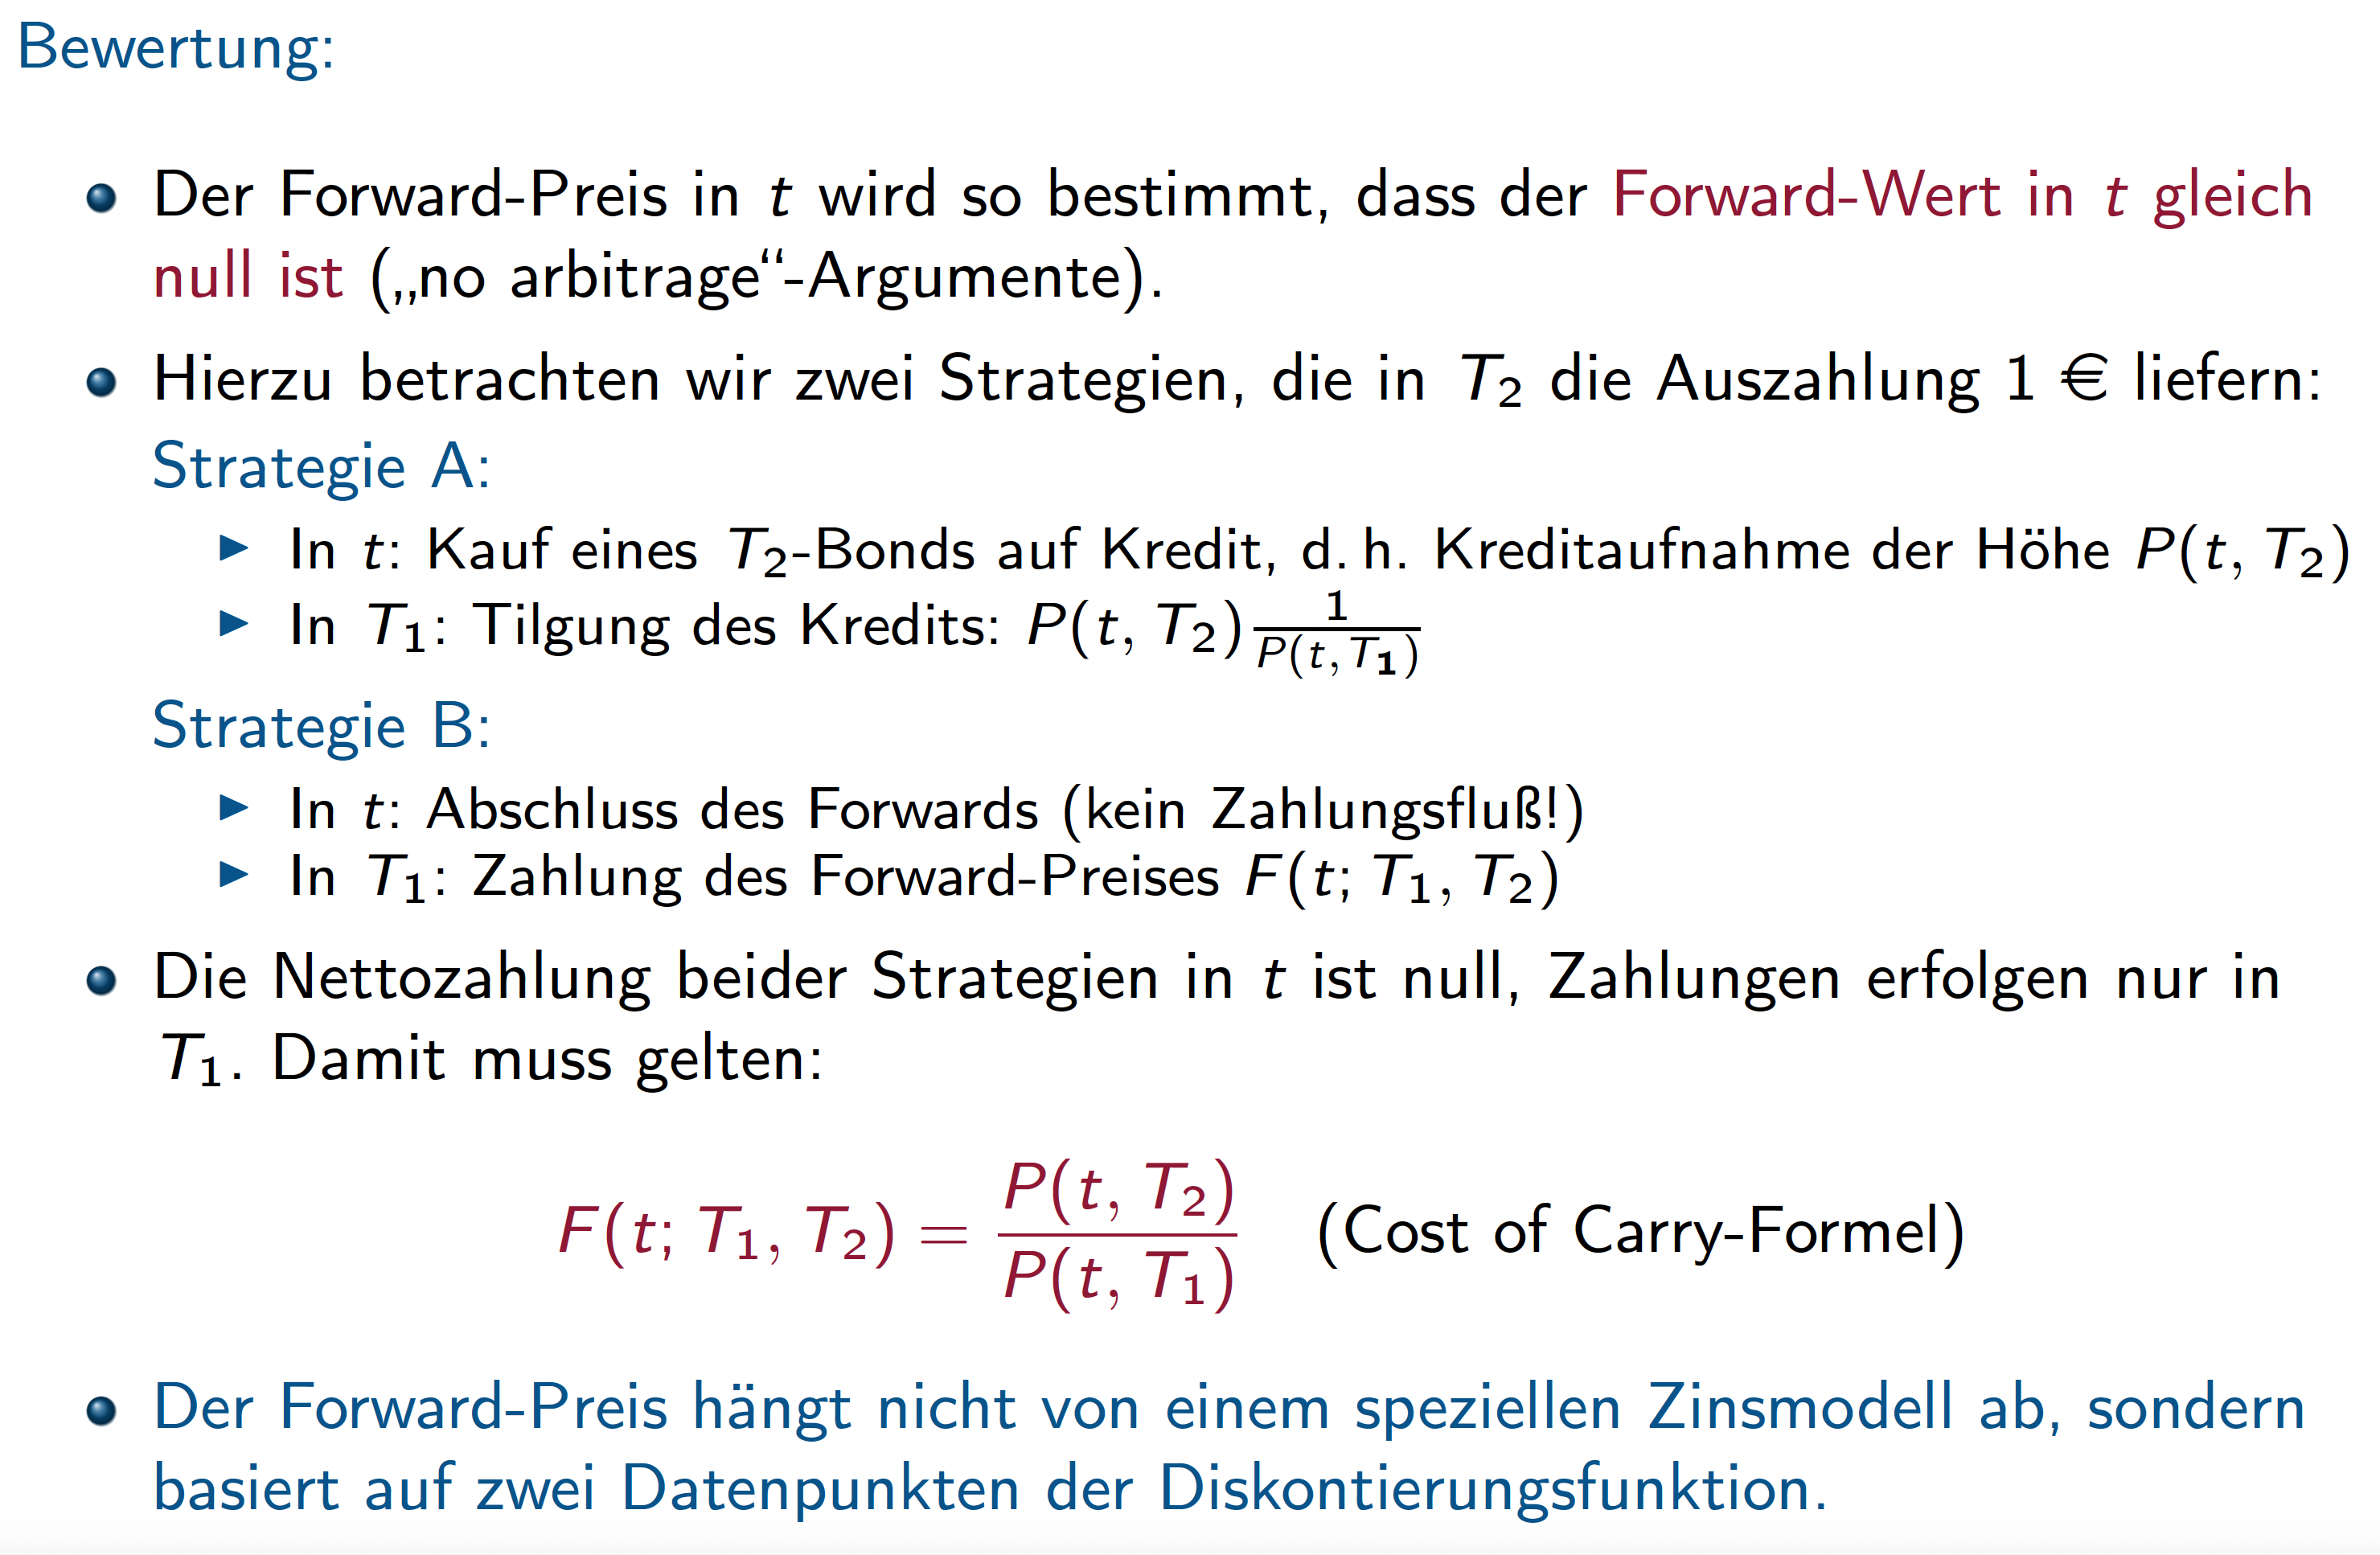
\includegraphics[width=\textwidth]{Bilder/FwdKontrakt2.png}
\end{figure}

\begin{figure}[H]
\centering
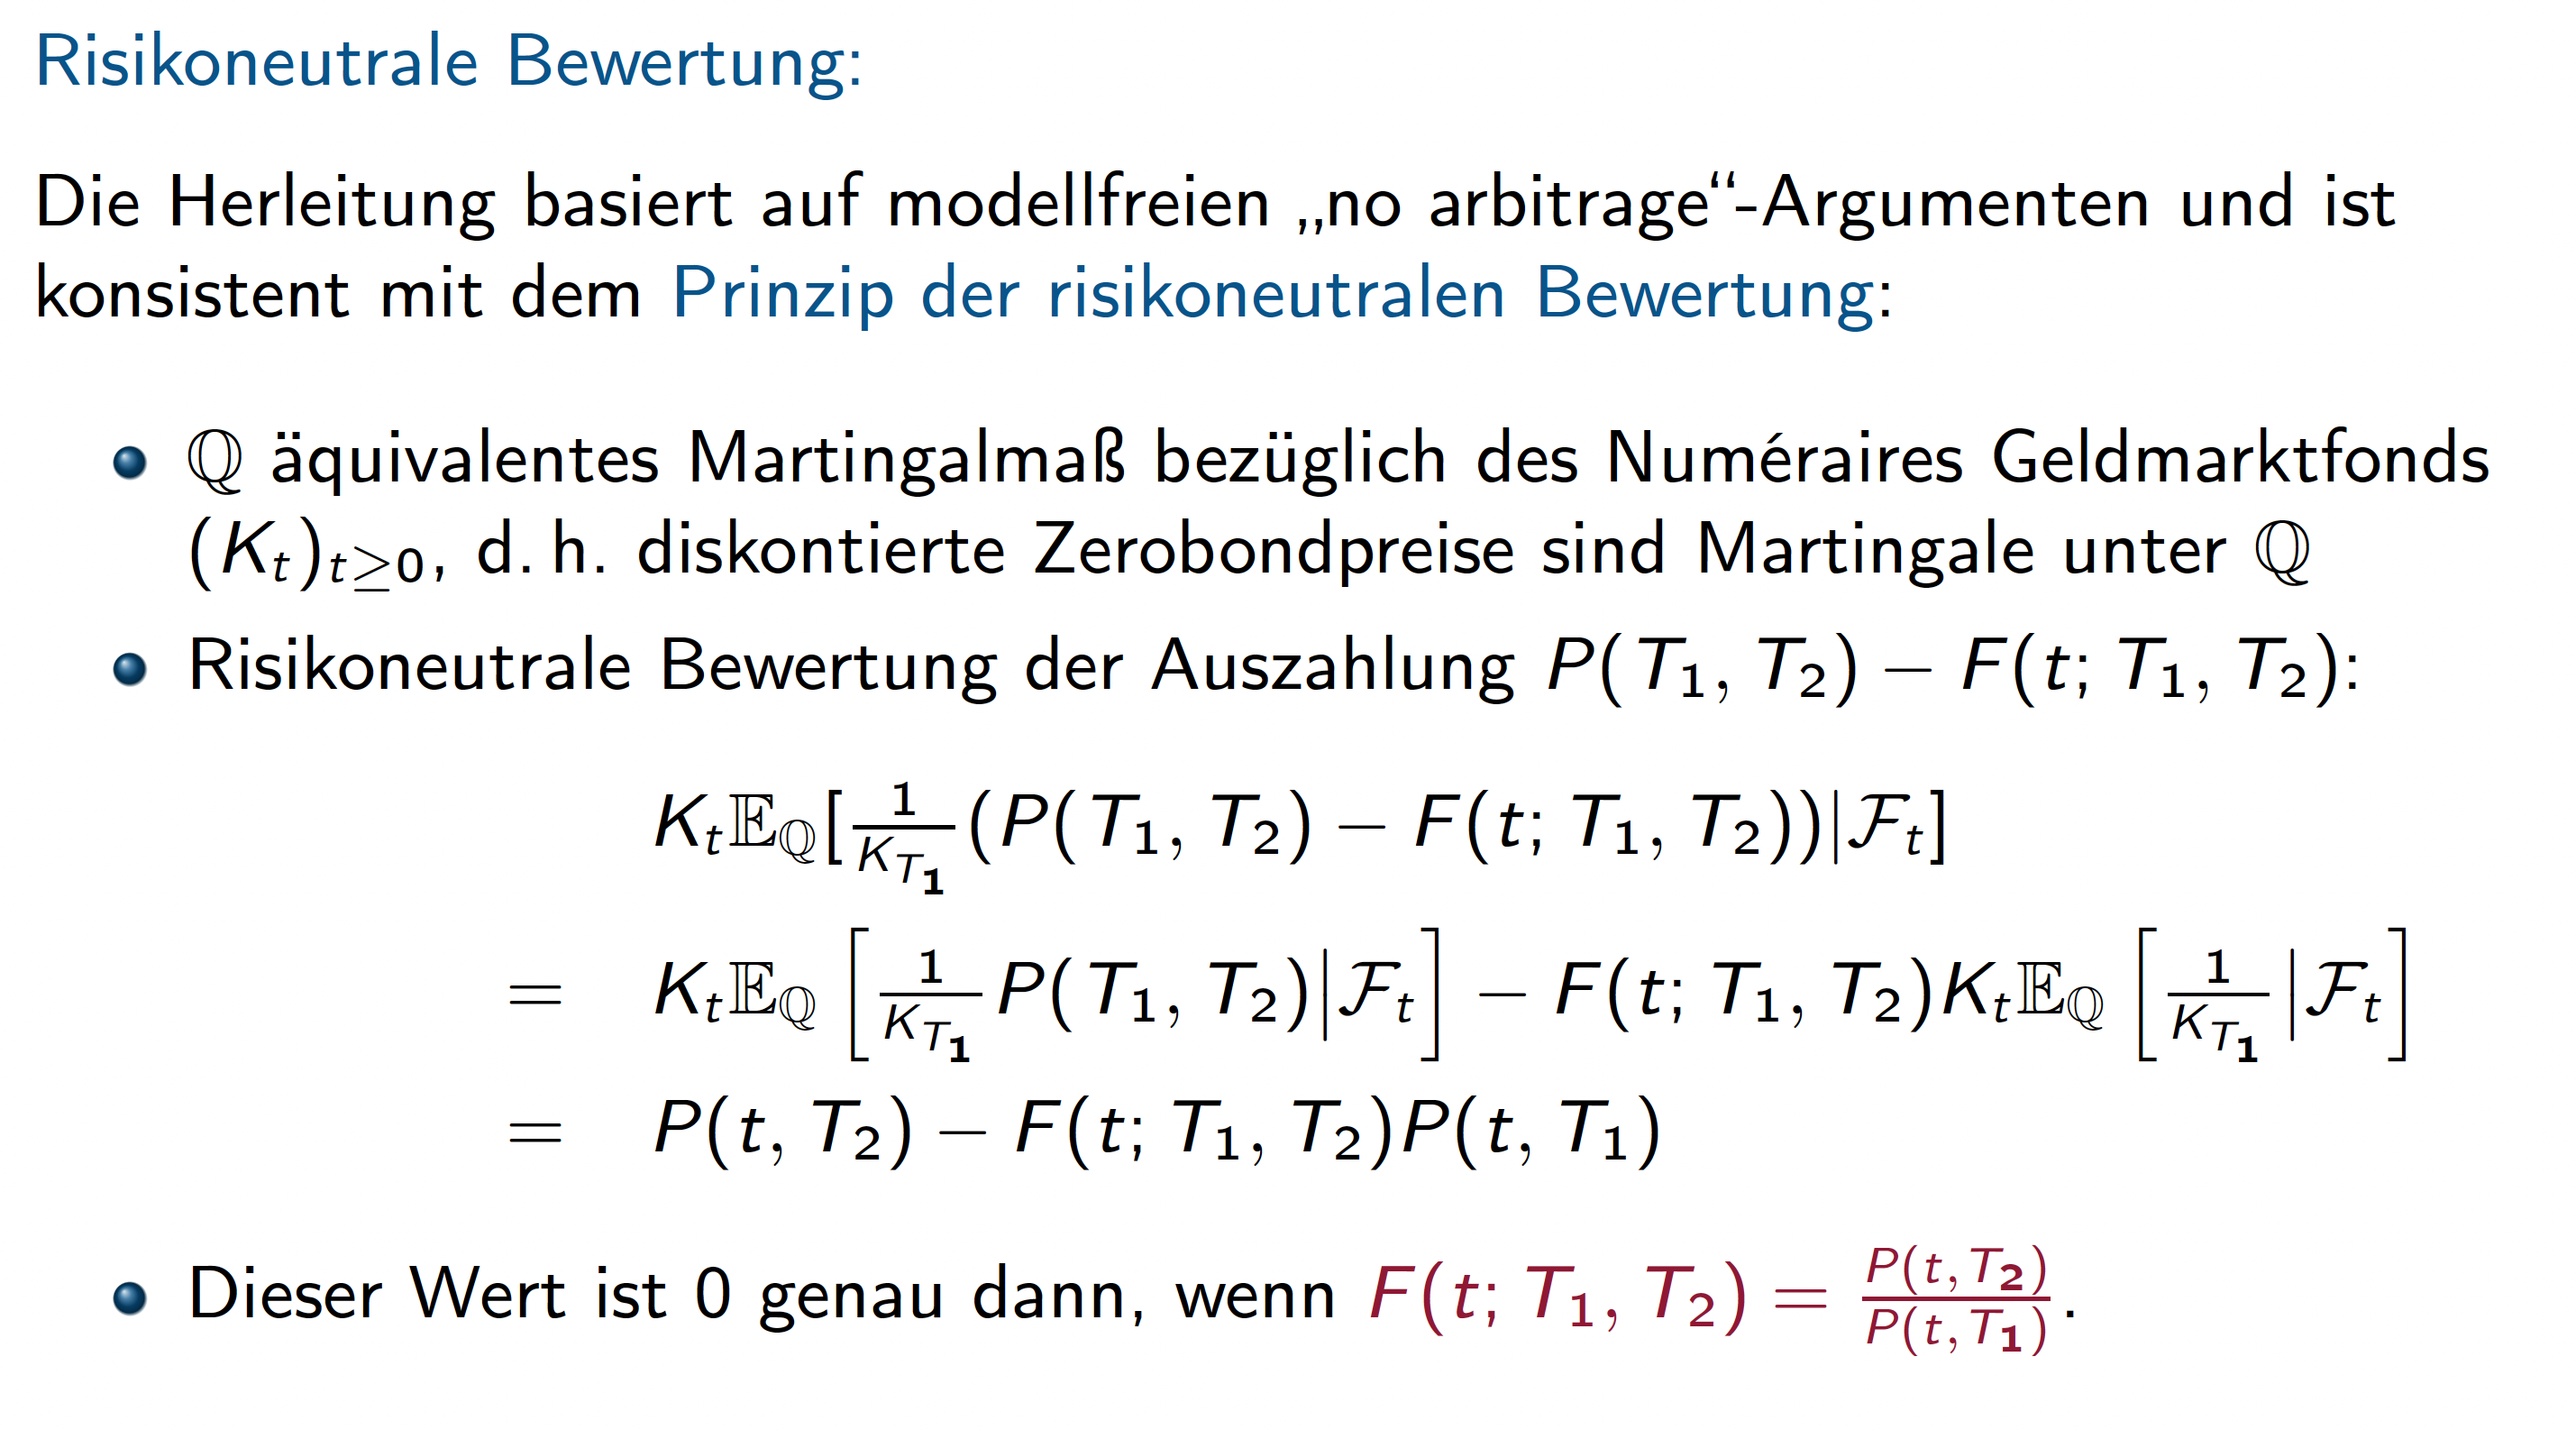
\includegraphics[width=\textwidth]{Bilder/FwdKontrakt3.png}
\end{figure}

\subsubsection{\"Uberblick Zinsswap}

\begin{itemize}
	\item Finanzderivat, bei dem zwei Parteien vereinbaren, zu vorher festgesetzten zuk\"unftigen Zeitpunkten Zinszahlungen auf Nennwerte zu tauschen
	\item Vereinfachung: Differenz zwischen Zinszahlungen wird getauscht
	\item Nennwerte stimmen i.d.R. \"uberein
	\item Zins-W\"ahrungs-Swap: Zinsswap auf verschiedenen W\"ahrungen
	\item Typisch: Austausch fester gegen variable Zinsen
	\item Zweck: Absicherung gegen Zins\"anderungen oder Spekulation auf diese
	\item Payer-Swap: Swap aus Sich der Vertragspartei, die den festen Zins zu zahlen hat und daf\"ur den variablen Zinssatz erh\"alt
	\item Receiver-Swap: Swap aus Sich der Vertragspartei, die den variablen Zins zu zahlen hat und daf\"ur den festen Zinssatz erh\"alt
	\item Wert Payer-Swap: $\Pi^p(t) = N(P(t,T_0) - P(t,T_n) - r \delta \sum_{k=1}^n P(t,T_k))$
	\item Wert Receiver-Swap: $\Pi^r(t) = - \Pi^p(t)$ entgegengesetzt zum Payer-Swap
	\item Forward Swap Rate: $\Pi^p(t) = - \Pi^r(t) = 0$
\end{itemize}

\section{Risikoneutrale Bewertung von Aktienderivaten in Binomialb\"aumen}

\subsection{Klassische Aktienderivate}

\begin{itemize}
	\item Aktienderivat: Finanzkontrakt, dessen Auszahlung (Zahlungsstrom) sich aus dem realisierten Kursverlauf einer Aktie ableitet
	\item Formal: $C_t = f(S_0,S_1,...,S_t)$ f\"ur eine Funktion $f$, $(S_t)_{t=0,1,...,T}$ der Aktienpreisprozess, $C_T$ die Auszahlung
	\item Beispiele:
	\begin{itemize}
		\item Call-Option: $C_T^{call} = S_T-K)^+$ mit Aus\"ubungspreis $K>0$
		\item Put-Option: $C_T^{put} = (K-S_T)^+$ mit Aus\"ubungspreis $K>0$
	\end{itemize}
\end{itemize}

\begin{figure}[H]
\centering
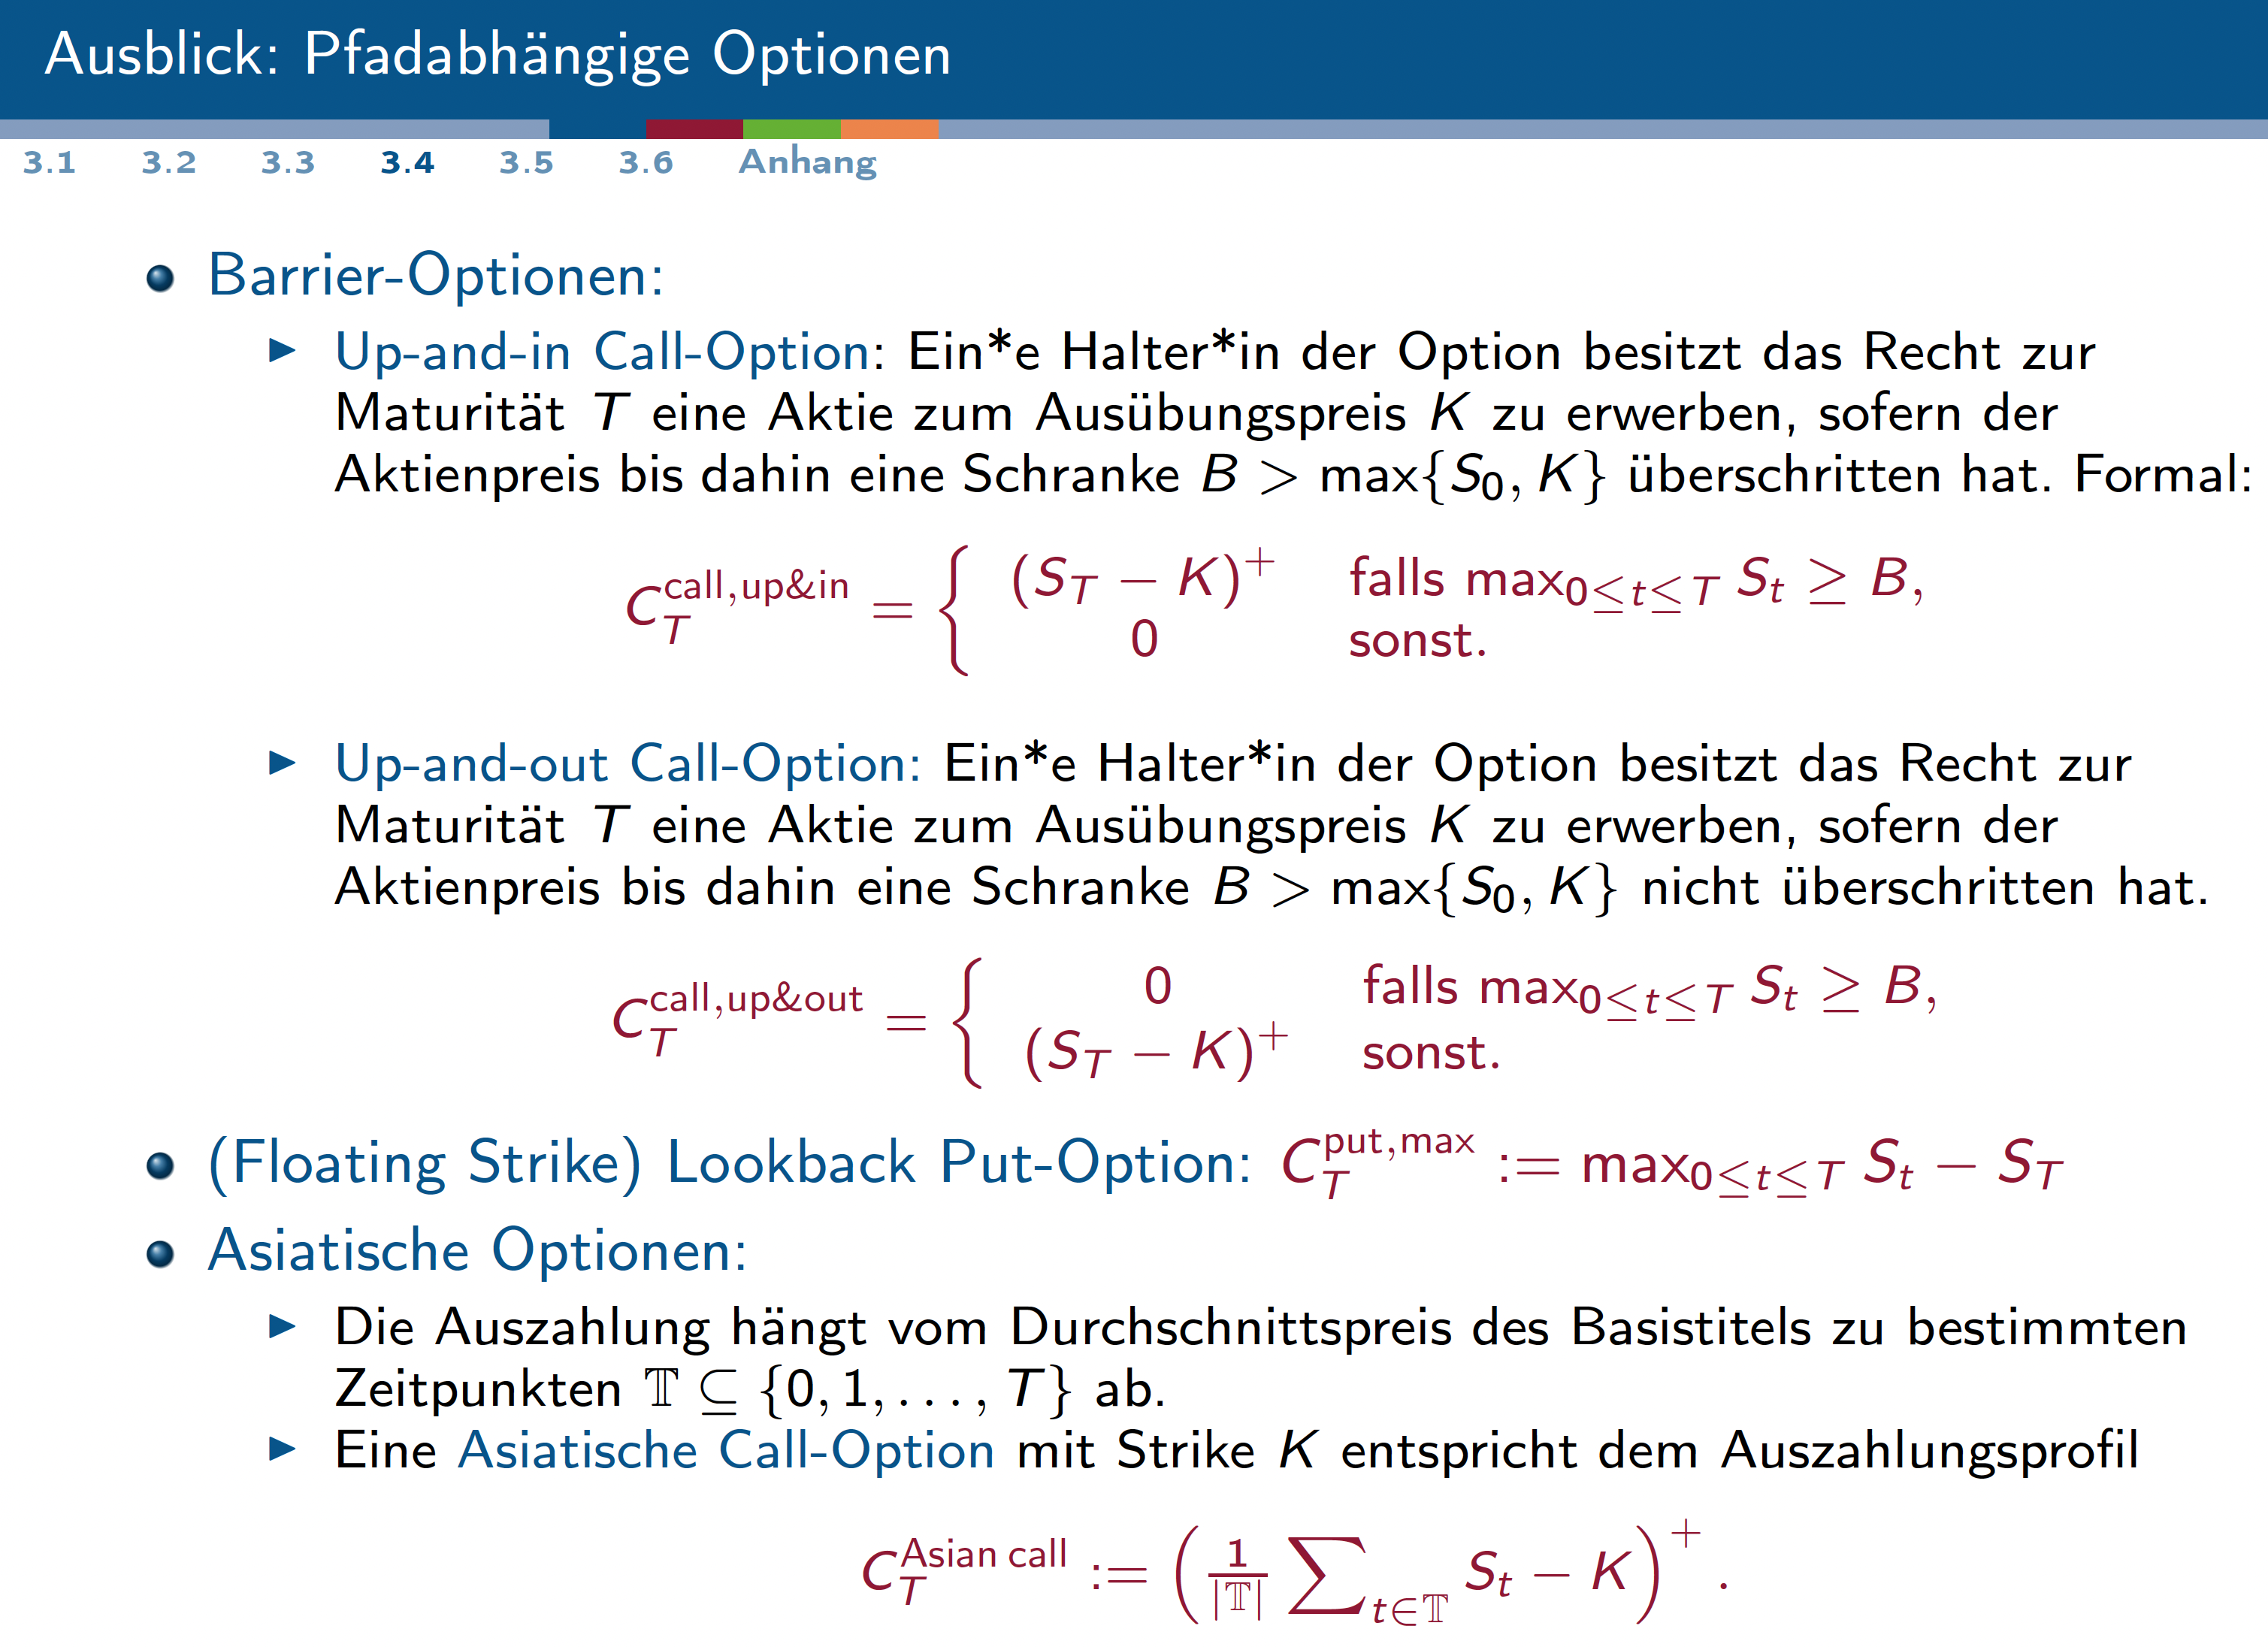
\includegraphics[width=\textwidth]{Bilder/AusblickOptionen.png}
\end{figure}

\subsubsection{Binomialmodell}

\subsubsection{Binomialmarktmodell nach Cox-Ross-Rubinstein}

\begin{itemize}
	\item diskretes Finanzmarktmodell mit $T$ Handelsperioden
	\item Prim\"are Produkte:
	\begin{itemize}
		\item Risikofreie Anlage (Sparbuch): deterministischer Periodenzins $r>-1$, \\ $S_t^0 := (1+r)^t$, $t=0,...,T$
		\item Risikobehaftete Anlage (Aktie): $S:=S^1$
		\begin{itemize}
			\item in jeder Handelsphase Up-Faktor $u$ oder Down-Faktor $d$ unterstellt
			\item Aktienpreis springt entweder auf h\"oheren Wert $S_t = S_{t-1} \cdot u$ oder niedrigeren Wert $S_t = S_{t-1} \cdot d$
		\end{itemize}
	\end{itemize}
\end{itemize}

\begin{figure}[H]
\centering
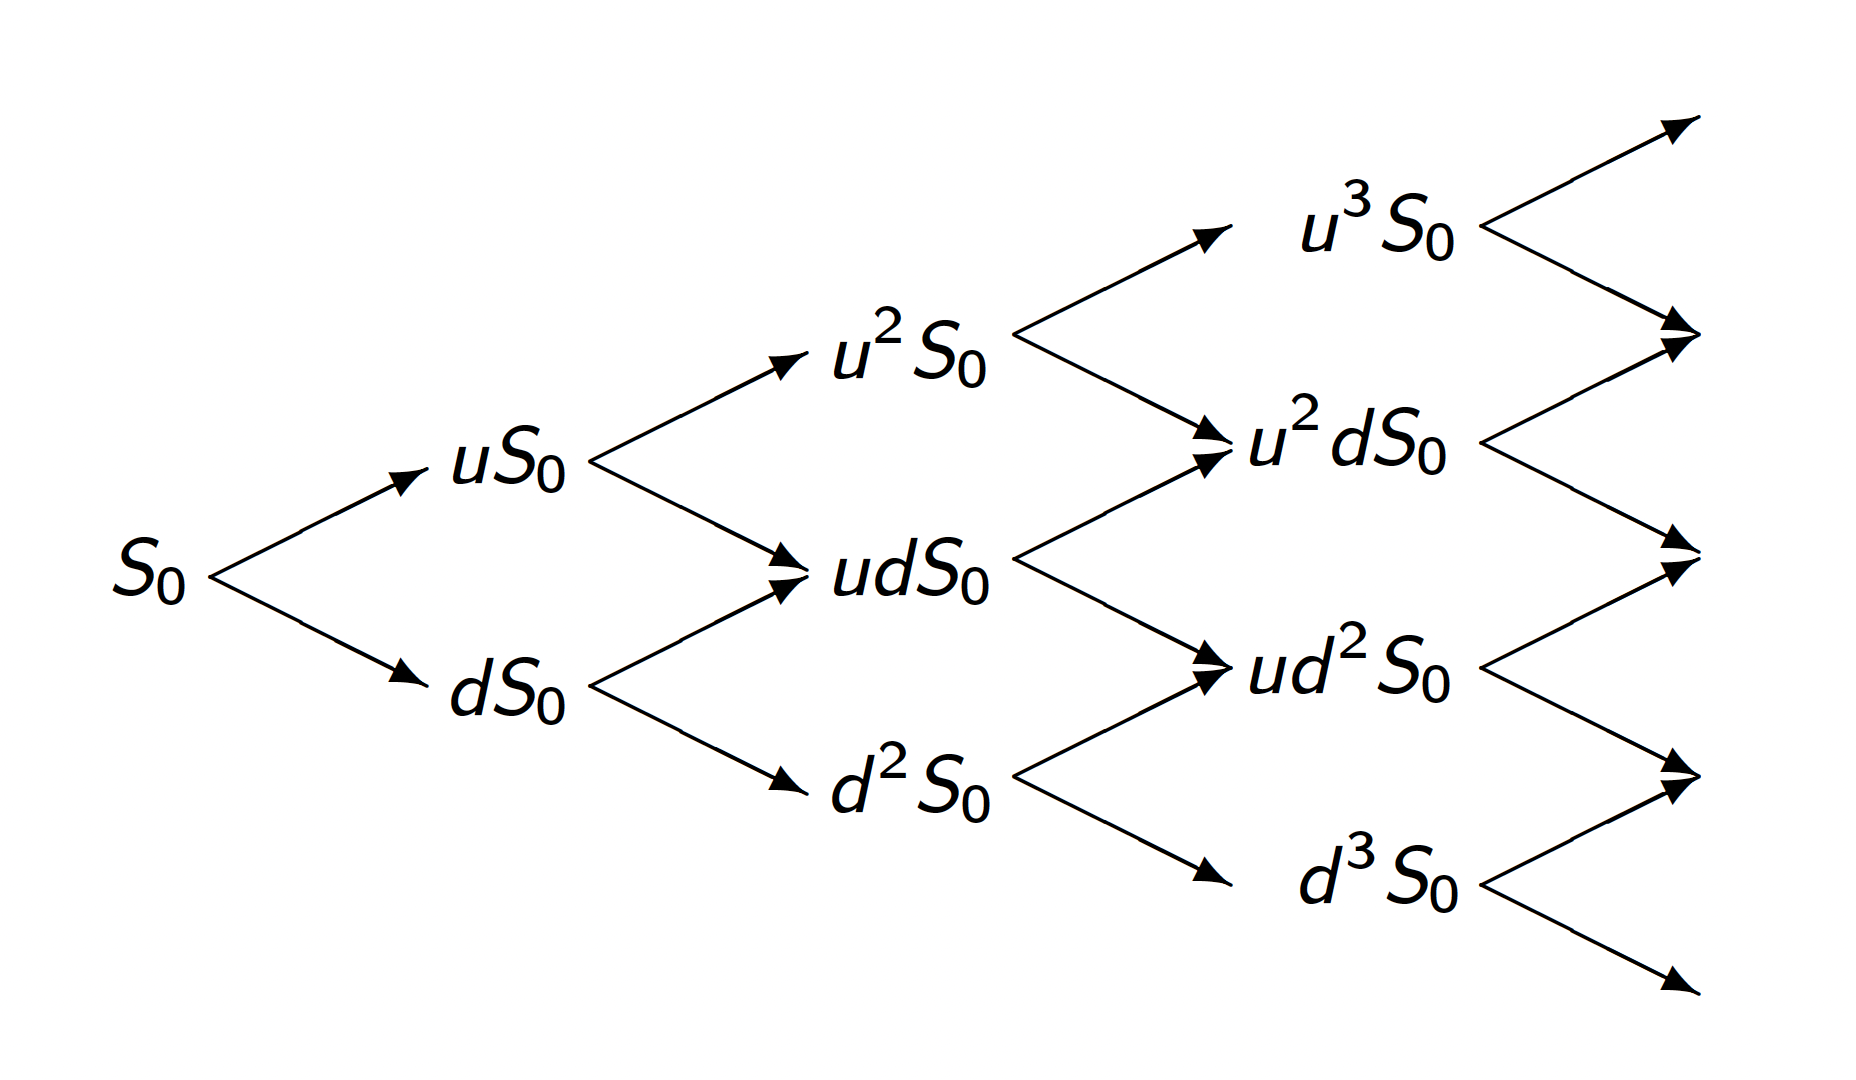
\includegraphics[width=\textwidth]{Bilder/BinomialmodellUpDown.png}
\end{figure}

\begin{figure}[H]
\centering
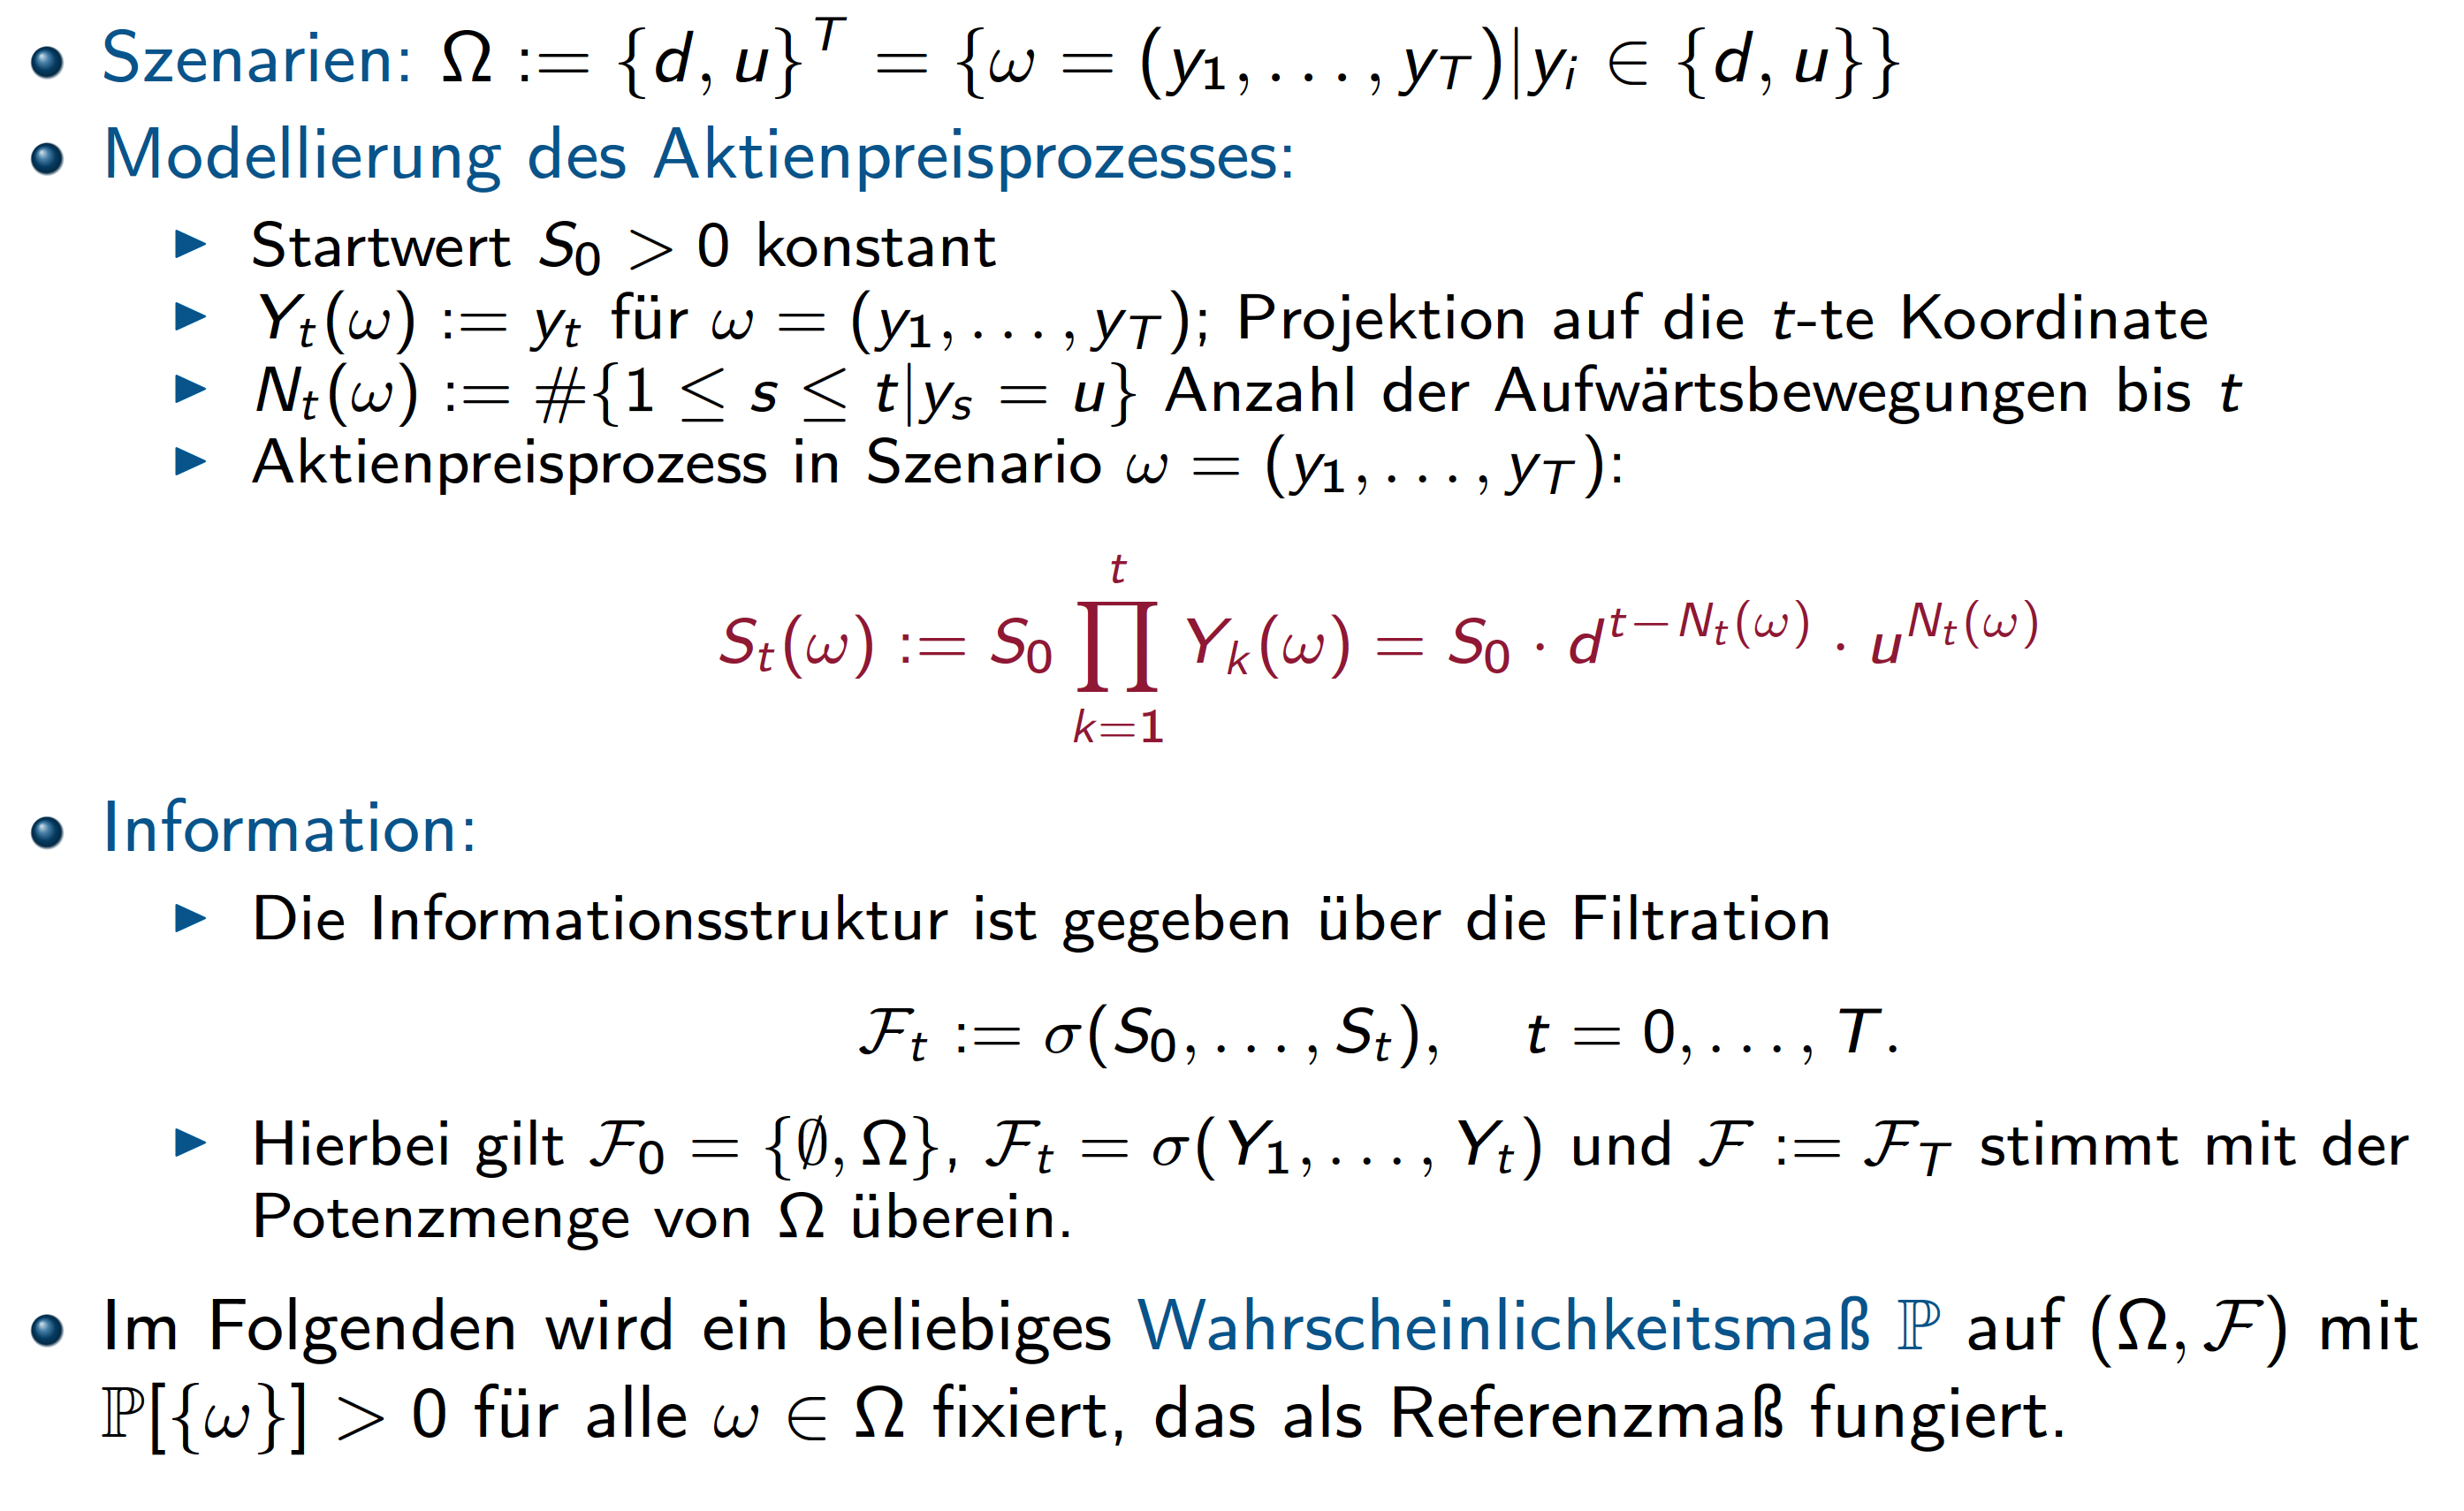
\includegraphics[width=\textwidth]{Bilder/FormaleKonstruktion.png}
\end{figure}

\begin{figure}[H]
\centering
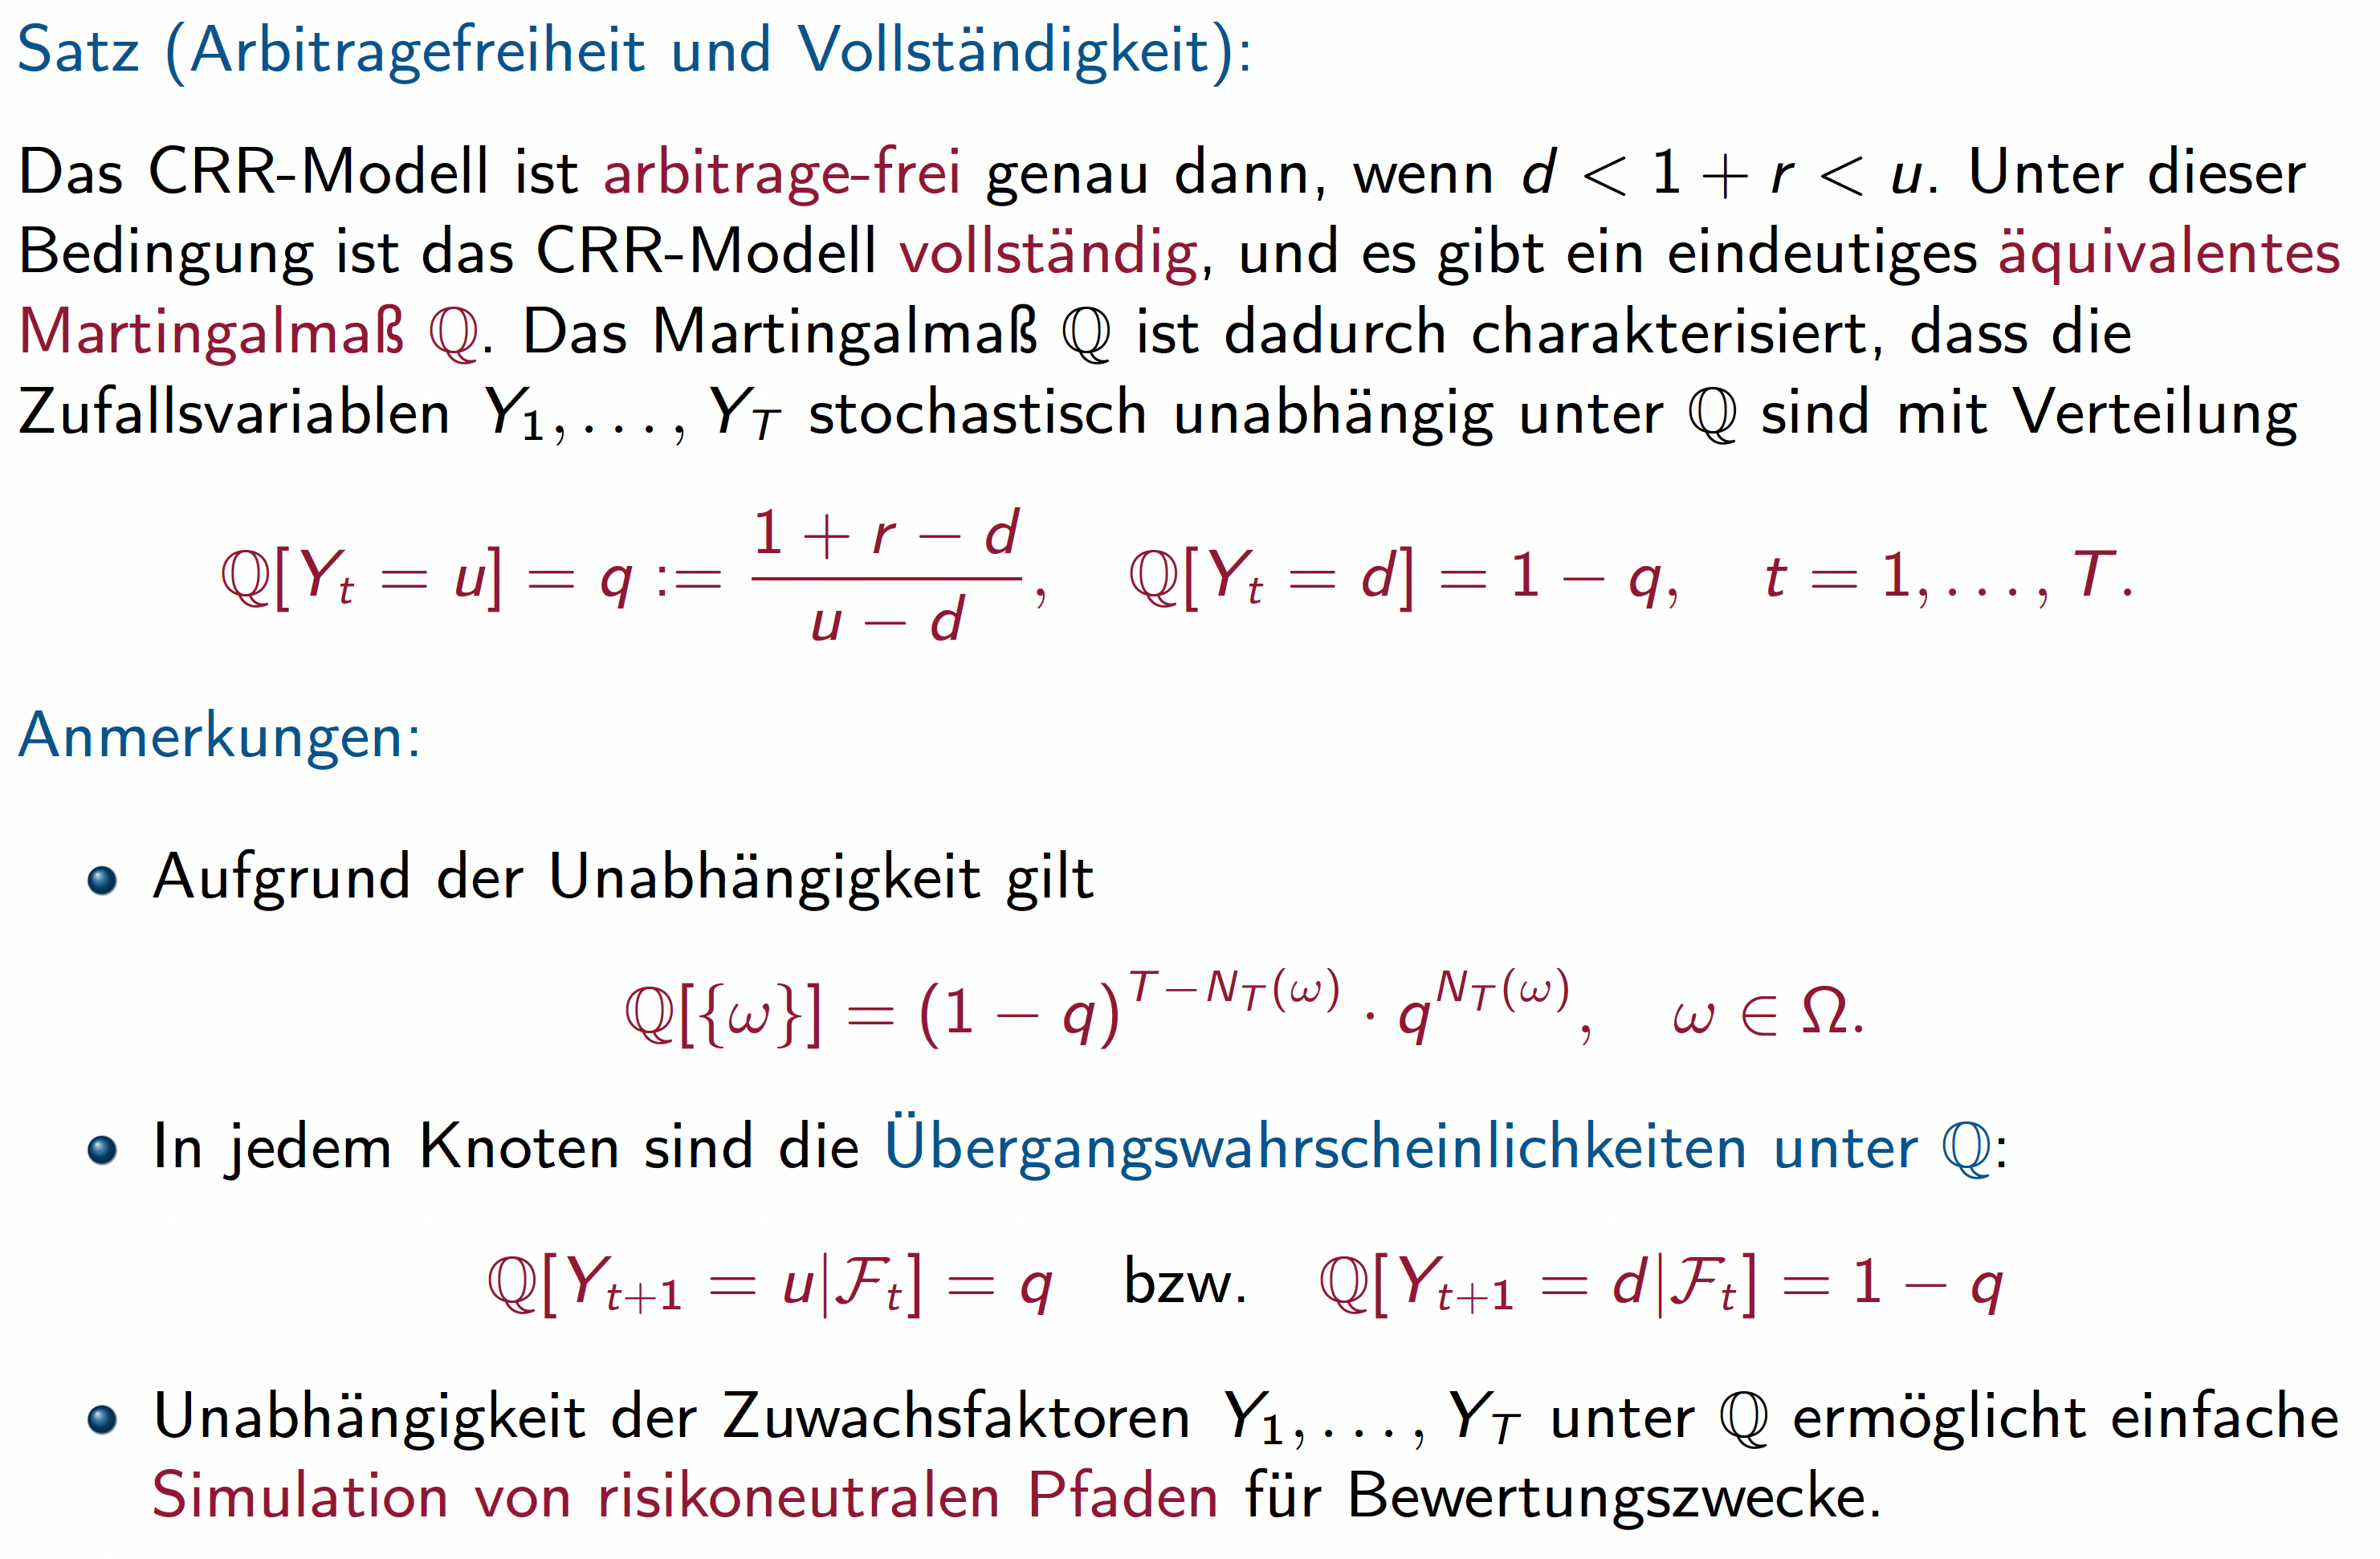
\includegraphics[width=\textwidth]{Bilder/SatzArbitragefreiheit.png}
\end{figure}

\begin{figure}[H]
\centering
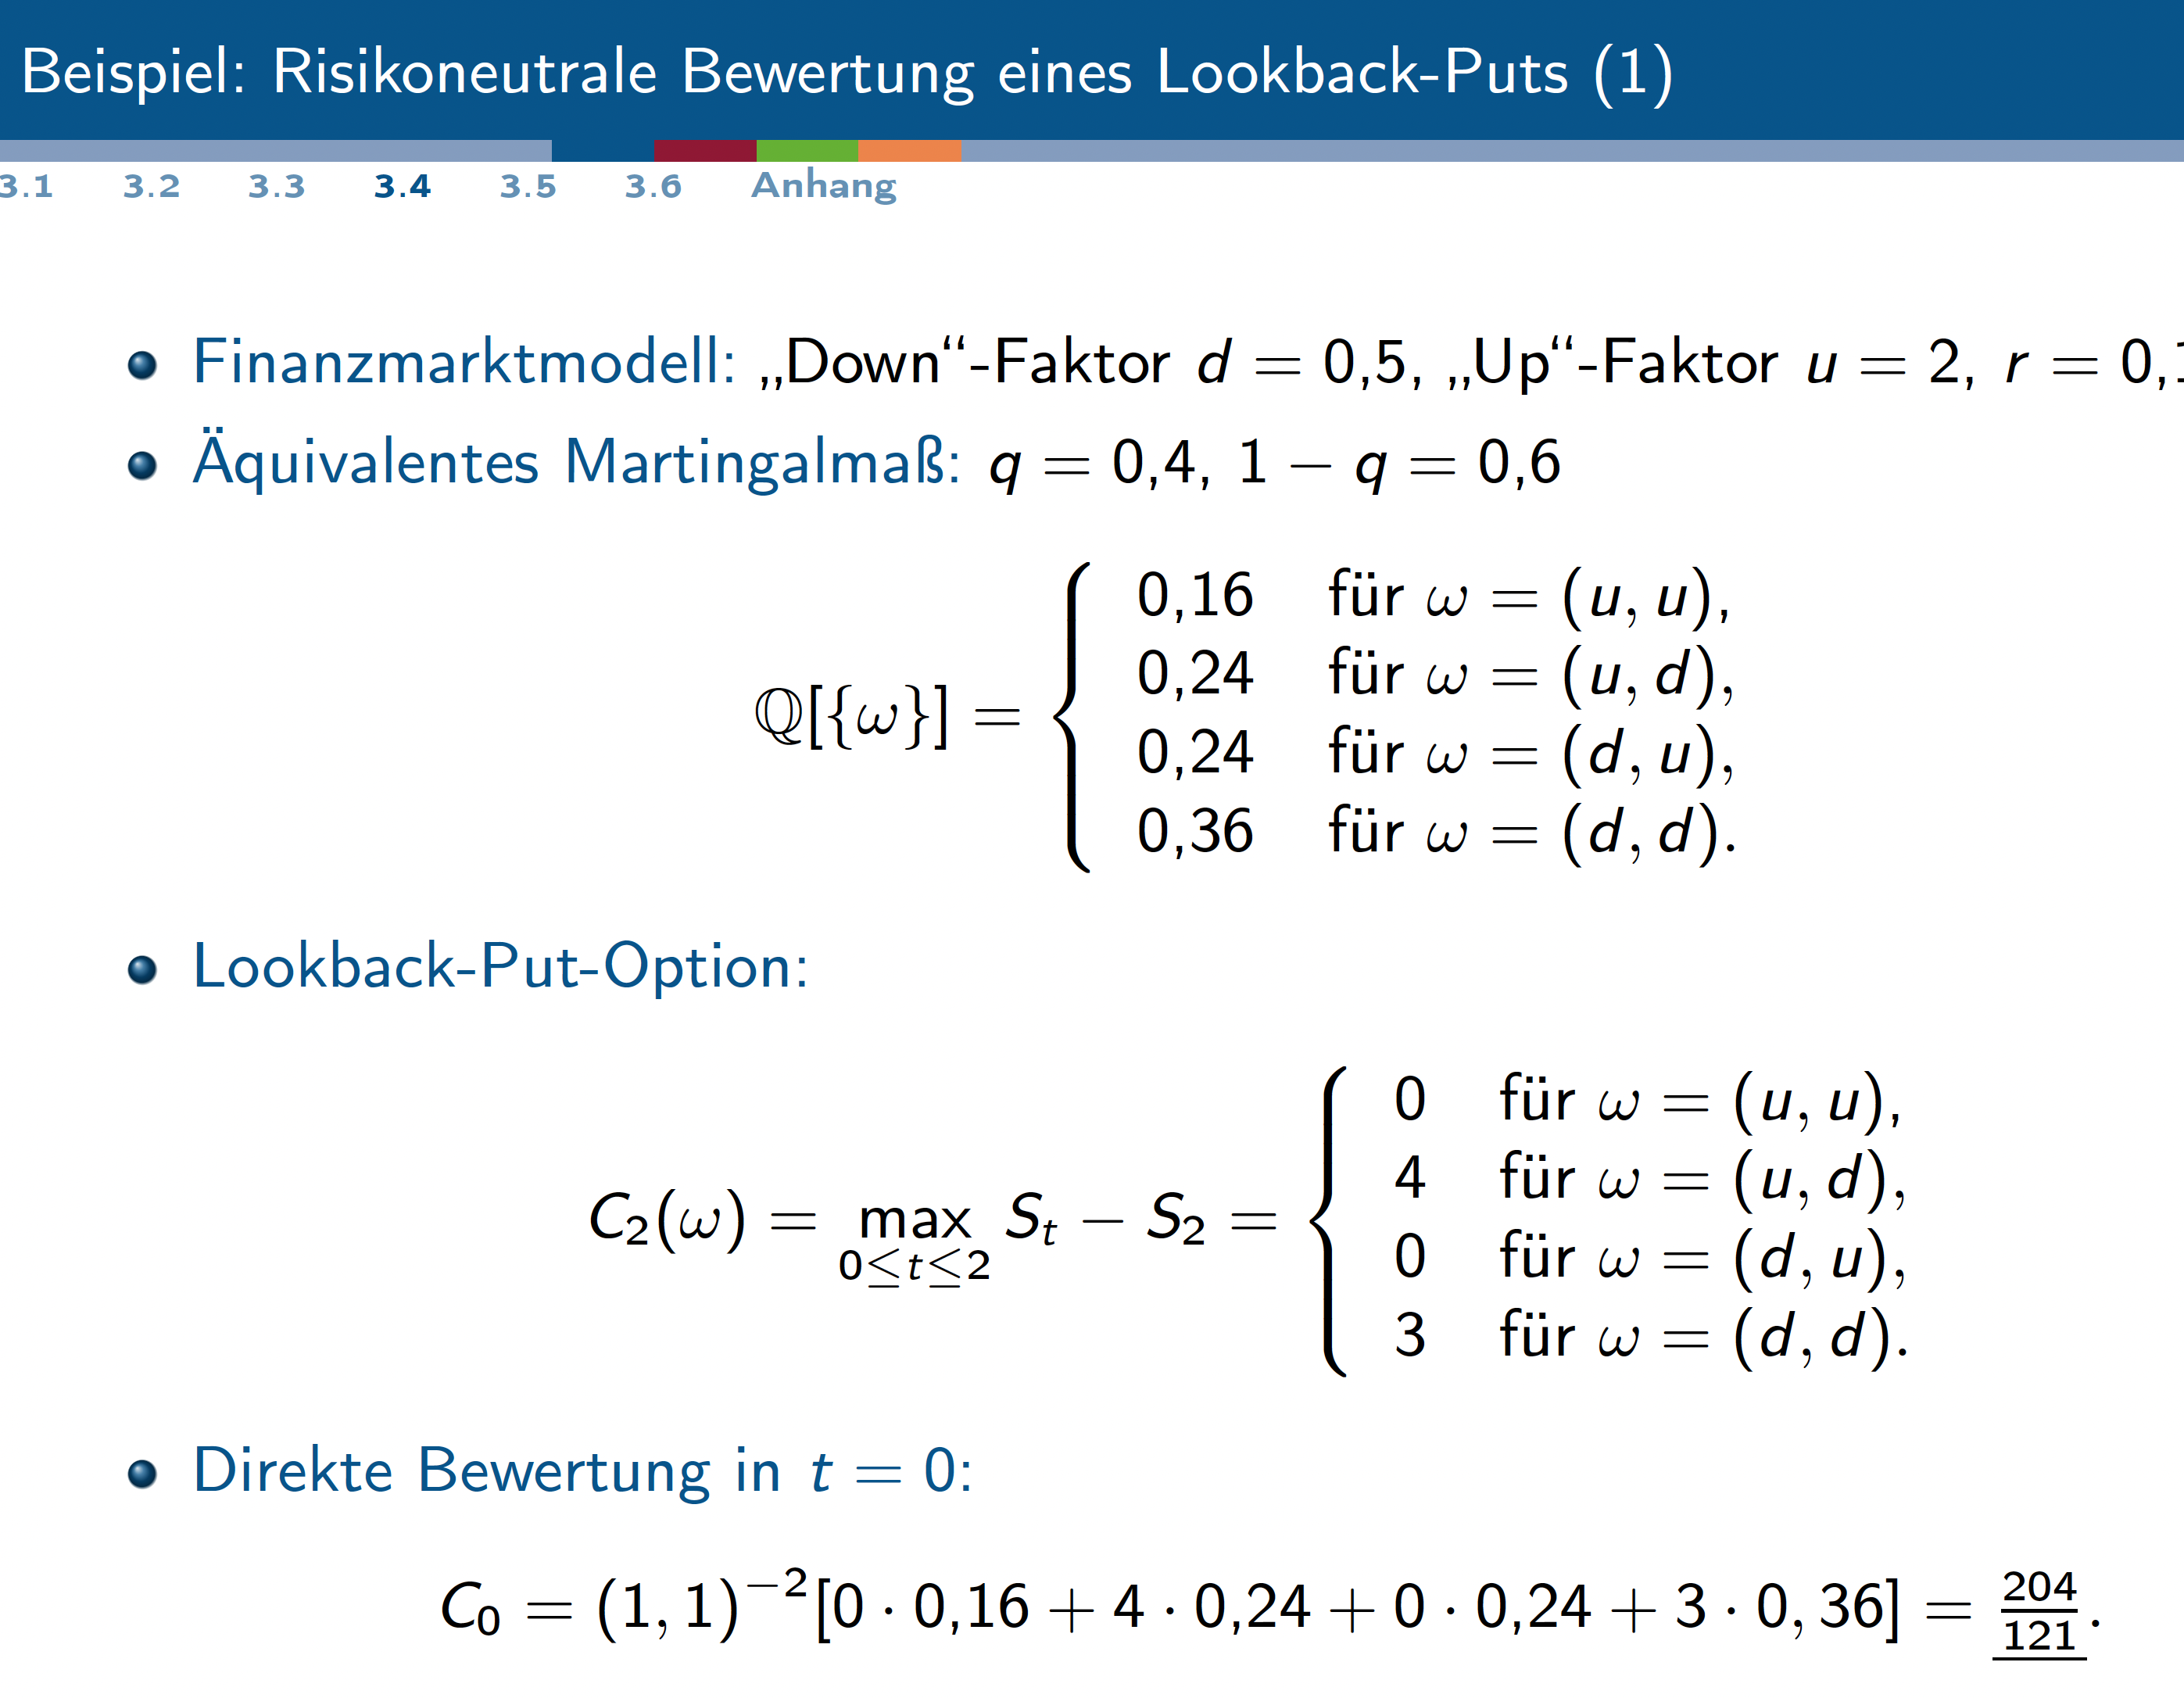
\includegraphics[width=\textwidth]{Bilder/LookbackPut.png}
\end{figure}











%----------------------------------------------------------------------

%KAPITEL 4

%----------------------------------------------------------------------



\chapter{Risiko und Risikomaße}

\section{Risiko und Knightian Uncertainty}

\begin{itemize}
\item Charakterisierung im Kontext der ökonomischen Entscheidungstheorie durch
Differenzierung zwischen „Risiko“ und „Unsicherheit“:
\begin{itemize}
\item "Risiko" bezieht sich auf Situationen, in denen das zugrunde liegende
Wahrscheinlichkeitsmaß $\mathcal{P}$ bekannt sind
\item ""Unsicherheit" stellt auf Fälle ab, in denen dies nicht der Fall 
\end{itemize}
\item Formalisierung Knight’scher Unsicherheit („Knightian Uncertainty“):
\begin{itemize}
\item Familie $\mathcal{P}$ von möglichen Wahrscheinlichkeitsmaßen statt eines Referenzmaßes
\item Jedes Element von P spiegelt eine mögliche Ausprägung der zugrunde
liegenden Wahrscheinlichkeitsverteilungen wider.
\end{itemize}
\item Standardvorgehen - Modellierung unter „Risiko“:
\begin{itemize}
\item Modellierung von Preisentwicklungen durch stochastische Prozesse, deren
Dynamik in der Regel bezüglich eines festen Maßes P spezifiziert ist.
\item Annahme: Investoren haben Kenntnis der
Wahrscheinlichkeitsverteilung der zugrunde liegenden Preisprozesse.
\end{itemize}
\item Realistischer - Knightian Uncertainty:
\begin{itemize}
\item Wahrscheinlichkeiten von Finanzmarktereignissen sind unbekannt.
\item Ohne Unsicherheit sollten Finanzinstitutionen in der Lage sein, Finanzprodukte
so zu bewerten, dass sie mögliche Verluste kontrollieren können.
\item Empirische Evidenz - wie etwa die Beobachtungen der Finanzmarktkrise vor
etwa einem Jahrzehnt - zeigen, dass dies von der Realität weit entfernt ist.
\end{itemize}
\end{itemize}


\section{Streuungsmaße und Risikomaße des Downside Risk}

\subsubsection{Risikomaße in der Praxis}
\begin{itemize}
\item Anwendungsfehler: 
\begin{itemize}
\item Pufferfunktion gegen adverse Entwicklungen (z. B. Solvabilitätskapitalanforderung)
\item Steuerungsfunktion (z. B. Limit- und Schwellenwertsystem)
\item Vergleichsfunktion für Finanzpositionen, Portfolien oder Unternehmen
\item Bewertungsfunktion
\end{itemize}
\item Kriterien für "gute" Risikomaße:
\begin{itemize}
\item Ökonomische Eigenschaften: adäquate Berücksichtigung von Diversifikation,
extremen Verlusten
\item Implementierung: umsetzbare Techniken für die statistische Schätzung von
Risikomaßen
\end{itemize}
\end{itemize}

\subsubsection{Risikomessung: Formalisierung}
\begin{itemize}
\item Finanzpositionen:
\begin{itemize}
\item $X$ Zufallsvariable auf einem Wahrscheinlichkeitsraum $(\Omega, \mathcal{F}, \mathbb{P})$, die den
(diskontierten) Wert einer Finanzposition am Ende einer vorgegebenen Periode
beschreibt
\item Voraussetzung: geeignete Integrierbarkeitsannahmen an $X$ 
\item Die Menge solcher Finanzpositionen wird mit $\mathcal{X}$ bezeichnet
\end{itemize}
\item Die Risikomessung erfolgt bezüglich des statistischen Maßes $\mathbb{P}$ („real-world“),
das die tatsächlichen Schwankungen widerspiegeln soll.
\item Ein Risikomaß ist allgemein ein Funktional 
\begin{equation}
\rho: \mathcal{X} \rightarrow \mathbb{R} \text{, } X \mapsto \rho(X)
\end{equation}
das einer Finanzposition $X$ eine Risikokennzahl $\rho(X)$ zuordnet.
\end{itemize}

\subsubsection{Streuungsmaße}
\begin{figure}[ht]
	\centering
	\includegraphics[width=0.9 \textwidth]{Bilder/Streuungsmaße.png}
\end{figure}

\begin{itemize}
\item Variationskoeffizient: $cv=\frac{\sigma(X)}{E(X)}$
\end{itemize}

\subsubsection{Momente}

\begin{figure}[ht]
	\centering
	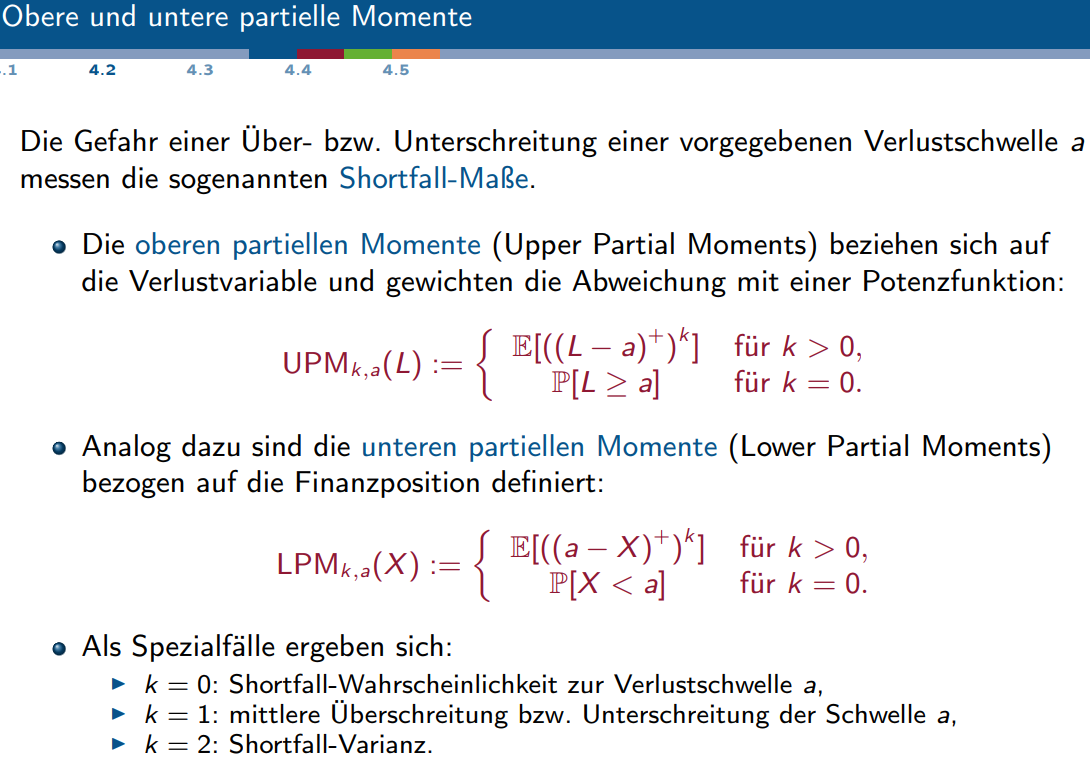
\includegraphics[width=0.9 \textwidth]{Bilder/Momente.png}
\end{figure}



\subsubsection{Value at Risk}
Value at Risk $\lambda \in (0,1)$ einer Finanzposition $X$:
\begin{equation}
VAR_\lambda(X) := inf\{m \in \mathbb{R}: \mathbb{P}[X+m<0]\leq \lambda\}
\end{equation}
\begin{itemize}
\item Der Parameter $\lambda \in (0,1)$ wird nahe 0 gewählt.
\item Kleinster Geldbetrag („Risikokapital“), den man zu $X$ hinzufügen muss,
sodass die Wahrscheinlichkeit eines Verlustes kleiner oder gleich $\lambda$ ausfällt.
\end{itemize}

Defizite:
\begin{itemize}
\item Extreme Verluste, die nur mit kleiner Wahrscheinlichkeit auftreten, werden vom
VaR völlig ausgeblendet.
\item VaR setzt keine angemessenen Anreize für die Diversifikation
\end{itemize}

Mean Value at Risk:
In der Praxis auf verwendet: $MVaR_\lambda(X) := VaR_\lambda(X-E(X))$ \\
Ist Grundlage für die Definition der SCR unter SII


\section{Axiomatische Theorie der Risikomaße}

\subsection{Risikomaße, Akzeptanzmenge und robuste Darstellung}

\subsubsection{Definition monetäres Risikomaß}
Ein Funktional $\rho: \mathcal{X} \rightarrow \mathbb{R}$ heißt monetäres Risikomaß, falls die folgenden Eigenschaften bestehen: 
\begin{itemize}
\item Inverse Monotonie: Ist $X(\omega) \leq Y(\omega)$ für alle $\omega \in \Omega$, so gilt $\rho(X) \geq \rho(Y)$
\item Geldinvarianz: Für jede reelle Zahl $m$ gilt $\rho(X+m)=\rho(X)-m)$
\end{itemize}

\subsubsection{Akzeptanzmenge eines monetären Risikomaßes}
\begin{itemize}
\item Eine Position $X \in \mathcal{X}$ ist akzeptabel für $\rho$, wenn $\rho(X)\leq 0$.
\item Die Menge $\mathcal{A}=\mathcal{A}_\rho$ aller akzeptablen Positionen heißt Akzeptanzmenge: $\mathcal{A} := \{X \in \mathcal{X}| \rho(X) \leq 0\}$
\item $\rho$ ist eine Kapitalanforderung, d. h. $\rho(X) = inf \{m \in \mathbb{R}|X+m\in \mathcal{A}\}$
\end{itemize}


\subsubsection{Diversifikation}
\begin{itemize}
\item Diversifikation ist eines der zentralen Prinzipien im Risikomanagement und in
der Portfolioselektion.
\item Um der Idee Rechnung zu tragen, dass Diversifikation das Risiko nicht
erhöhen sollte, ist folgende Anforderung natürlich:
\begin{equation}
\rho(\lambda X + (1-\lambda)Y) \leq max \{ \rho(X), \rho(Y)\} \text{ für } X,Y \in \mathcal{X} \text{ und } \lambda\in (0,1)
\end{equation}
\item Die Akzeptanzmenge $\mathcal{A}$ is konvex.
\item $\rho$ ist ein konvexes Funktional $\mathcal{X}$:
\begin{equation}
\rho(\lambda X + (1-\lambda ) Y ) \leq \lambda\rho (X) + (1-\lambda) \rho(Y) \text{ für } X,Y \in \mathcal{X} \text{ und } \lambda\in (0,1)
\end{equation}
\end{itemize}


\subsubsection{Definition konvexes Risikomaß}
\begin{itemize}
\item Ein monetäres Risikomaß $\rho$ auf $\mathcal{X}$ heißt konvexes Risikomaß, falls es ein konvexes Funktional ist und damit Diversifikation nicht bestraft.
\item Ein konvexes Risikomaß wird kohärent genannt, falls es zusätzlich positiv
homogen ist, d. h. es gilt $\rho(\lambda X) = \lambda\rho(X)$ für alle $X \in \mathcal{X}$ und $\lambda\geq 0$
\end{itemize}


\subsubsection{Robuste Darstellung konvexer Risikomaße}

\begin{figure}[ht]
	\centering
	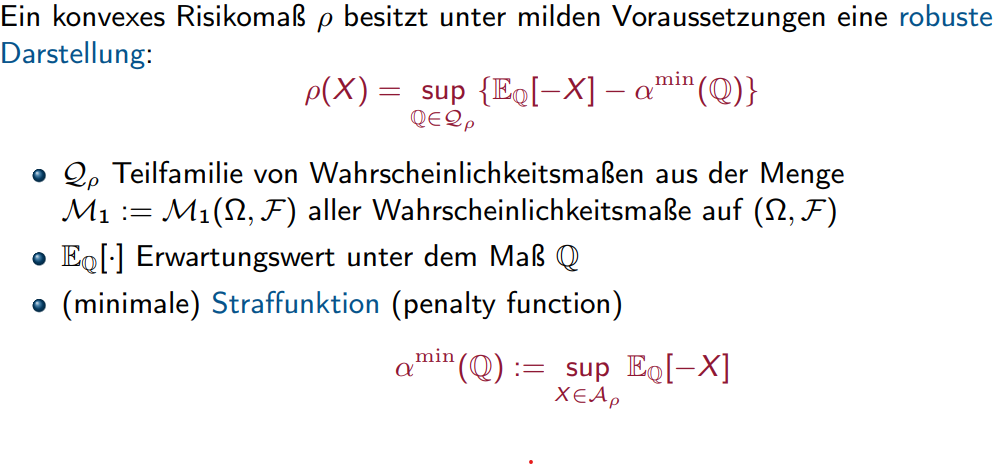
\includegraphics[width=0.9 \textwidth]{Bilder/robust.png}
\end{figure}

\subsubsection{Verteilungsbasierte Risikomaße}

\begin{figure}[ht]
	\centering
	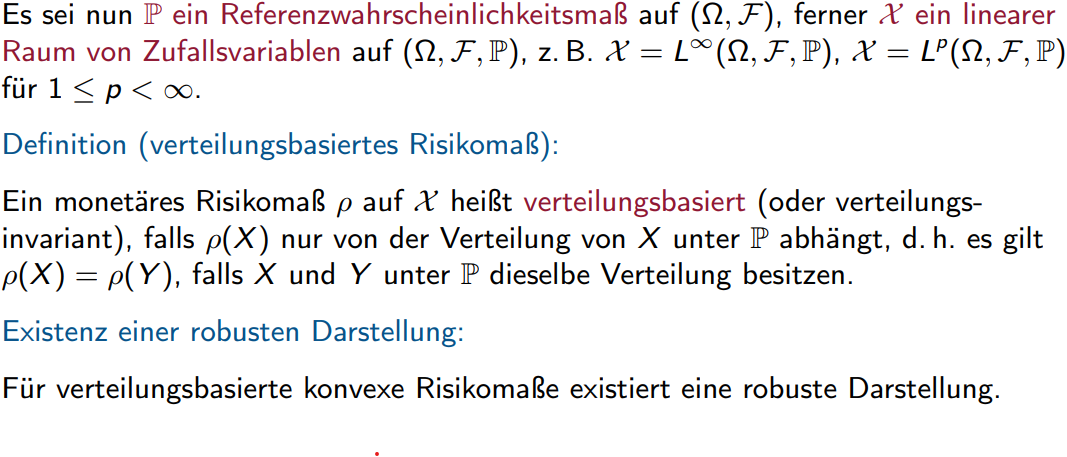
\includegraphics[width=0.9 \textwidth]{Bilder/verteilungsbasiert.png}
\end{figure}

\subsubsection{Value at Risk - Normalverteilung}

\begin{figure}[ht]
	\centering
	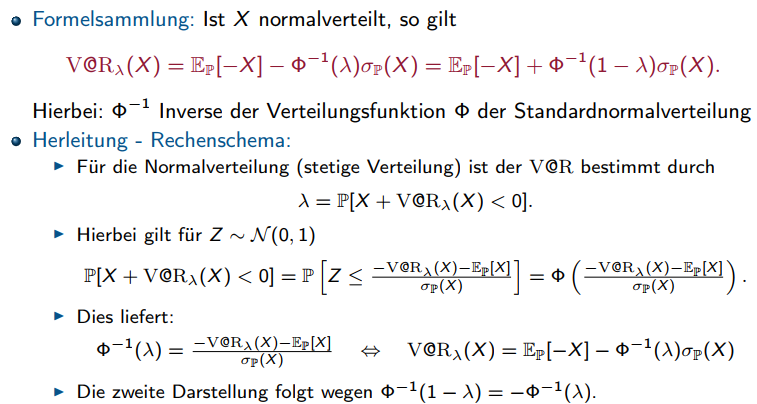
\includegraphics[width=0.9 \textwidth]{Bilder/VaR_Normal.png}
\end{figure}


\subsubsection{Average Value at Risk}
\begin{figure}[ht]
	\centering
	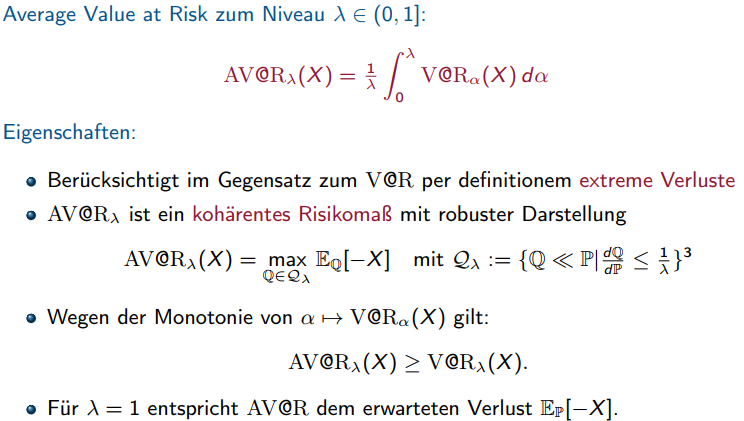
\includegraphics[width=0.9 \textwidth]{Bilder/AVaR.png}
\end{figure}


\subsection{Tail Value ar Risk}
\begin{figure}[ht]
	\centering
	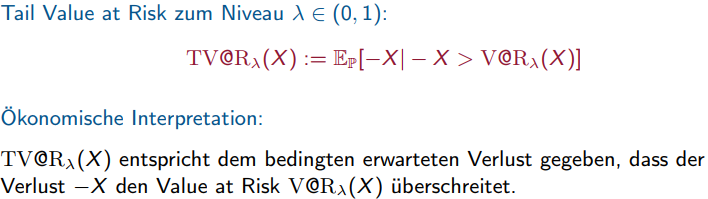
\includegraphics[width=0.9 \textwidth]{Bilder/TVaR.png}
\end{figure}

\subsection{Berechnung des erforderlichen Risikokapitals mit Risikomaßen}

Quantifizierbare Risiken: Marktrisiken, Ausfallrisiken (Herausforderungen: Datenqualität, Abhängigkeiten, operationelle Risiken) \\
Qualitativ bewertete Risiken: Emerging Risks, Strategische Risiken (Bewertung auf Expertenschätzung)

\subsection{Risikomessung unter SII}

\begin{itemize}
\item Drei Säulen: Quantitative Anforderungen (Vt. Rückstellungen, SCR), Qualitative Anforderungen (ORSA-Prozess, Risikomanagementsystem), Berichterstattung (SFCR, ORSA-Bericht)
\item Die Basiseigenmittel - definiert als Differenz von Assets und Liabilities gemäß
Solvenzbilanz - werden mit $E_0$ bzw. $E_1$ bezeichnet.
\begin{itemize}
\item Basiseigenmittel $E_0$ zu $t = 0$ sind deterministisch
\item Basiseigenmittel $E_1$ im Einjahreshorizont sind stochastisch
\end{itemize}
\item Vorgabe: SCR muss ausreichend sein, um einem Ruin im Einjahreshorizont mit der
Wahrscheinlichkeit $99,5 \%$ vorzubeugen
\item \begin{figure}[ht]
	\centering
	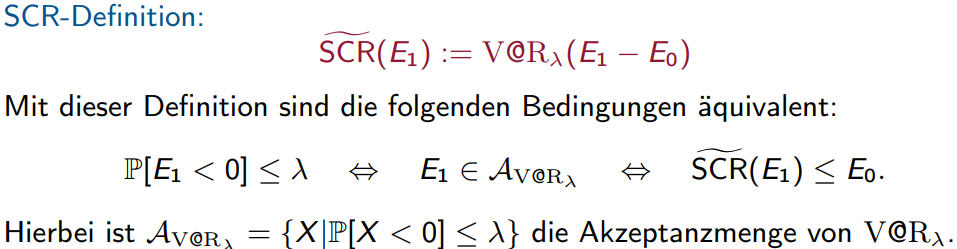
\includegraphics[width=0.9 \textwidth]{Bilder/SCR.png}
\end{figure}
\item Mean Value at Risk der Basiseigenmittel $E_1$:
\begin{equation}
SCR(E_1) = VaR_{0,005}(E_1- E(E_1))
\end{equation}
\item Standardformel:
\begin{itemize}
\item Modularer Aufbau: operationelles Risiko und
Risikomodule „nichtlebensvt. Risiko“, „lebensvt.
Risiko“, „krankenvt. Risiko“, „Marktrisiko“ und
„Gegenparteiausfallrisiko“ der
Basissolvabilitätskapitalanforderung 
\item Risikoaggregation per Wurzelformel
\end{itemize}
\item Internes Modell:
\begin{itemize}
\item Implementierung in komplexen Simulationsmodellen
\item Genehmigung durch Aufsicht (BaFin) notwendig
\end{itemize}
\end{itemize}






%----------------------------------------------------------------------

%KAPITEL 5

%----------------------------------------------------------------------



\chapter{Portfoliooptimierung}

\section{Nutzenoptimierung}

\subsection{Nutzenbasierte Portfoliooptimierung}

\subsubsection{Ausgangslage: Finanzpositionen}
\begin{itemize}
	\item Ein Investor hat das Ziel, ausgehend von einem Startkapital $v>0$, den Wert des Verm\"ogens zu einem Zeitpunkt $T$ zu optimieren
	\item Weitere Kapitalzuf\"uhrungen ider -entnahmen sind nicht vorgesehen
	\item Das Verm\"ogen $V$ zum Zeitpunkt $T$ kann mit einer reellwertigen Zufallsvariablen auf einem messbaren Raum identifiziert werden
	\item F\"ur Investitionen steht eine Menge $\mathcal{X}$ solcher Positionen zur Auswahl
\end{itemize}

\subsubsection{Pr\"aferenzordnung}

\begin{itemize}
	\item Die Pr\"aferenzordnung $\succ$ auf $\mathcal{X}$ sei \"uber das Pr\"aferenzfunktional $\mathcal{U}(X) = \mathbb{E_P}[x(X)]$ expliziert
	\item $X \succ Y \Leftrightarrow \mathbb{E_P}[x(X)] > \mathbb{E_P}[x(Y)]$, $(X,Y \in \mathcal{X})$
	\item $\mathbb{P}$ ein Referenzwahrscheinlichkeitsma{\ss}
	\item $u$ eine Nutzenfunktion
	\item Annahme: risikoaverses Verhalten der Investoren
	\item Nutzenfunktion einer risikoaversen Person: $u:S \subset \mathbb{R} \rightarrow \mathbb{R} \cup \{\infty\}, \ x \rightarrow x(x)$, falls $u$ strikt konkav und strikt wachsend auf $S$
	\item Um die Positionen in $\mathcal{X}$ zu realisieren kann der Investor:
	\begin{itemize}
		\item geeignete Portfolios aus prim\"aren Finanzprodukten konstruieren
		\item mit derivaten Produkten handeln
	\end{itemize}
	\item vollst\"andiger Markt: gleiche Menge erreichbarer Positionen mit beiden F\"allen
	\item unvollst\"andiger Markt: Derivate bieten mehr Flexibilit\"at
\end{itemize}



\section{Portfoliotheorie nach Markowitz}

\subsection{Grundlagen}

\begin{itemize}
	\item Ausgangspunkt: Universum aus $n$ Finanztiteln
	\item Risikoebene: Diversifikation
	\item Risiko/Wert-Ebene: Rendite/Risiko-Dominanz und effiziente Portfolios
	\item Ein Portfolio mit Rendite $R_1$ dominiert ein Portfolio mit Rendite $R_2$, wenn entweder \\ $Var(R_1) < Var(R_2)$ und $\mathbb{E}[R_1] \geq \mathbb{E}[R_2]$ \\ oder \\ $\mathbb{E}[R_1] > \mathbb{E}[R_2]$ und $Var(R_1) \leq Var(R_2)$
	\item Portfolio EV-effizient, wenn es durch kein anderes Portfolio dominiert wird
	\item nur effiziente Portfolios k\"onnen optimale Portfolios sein
\end{itemize}

\begin{figure}[H]
\centering
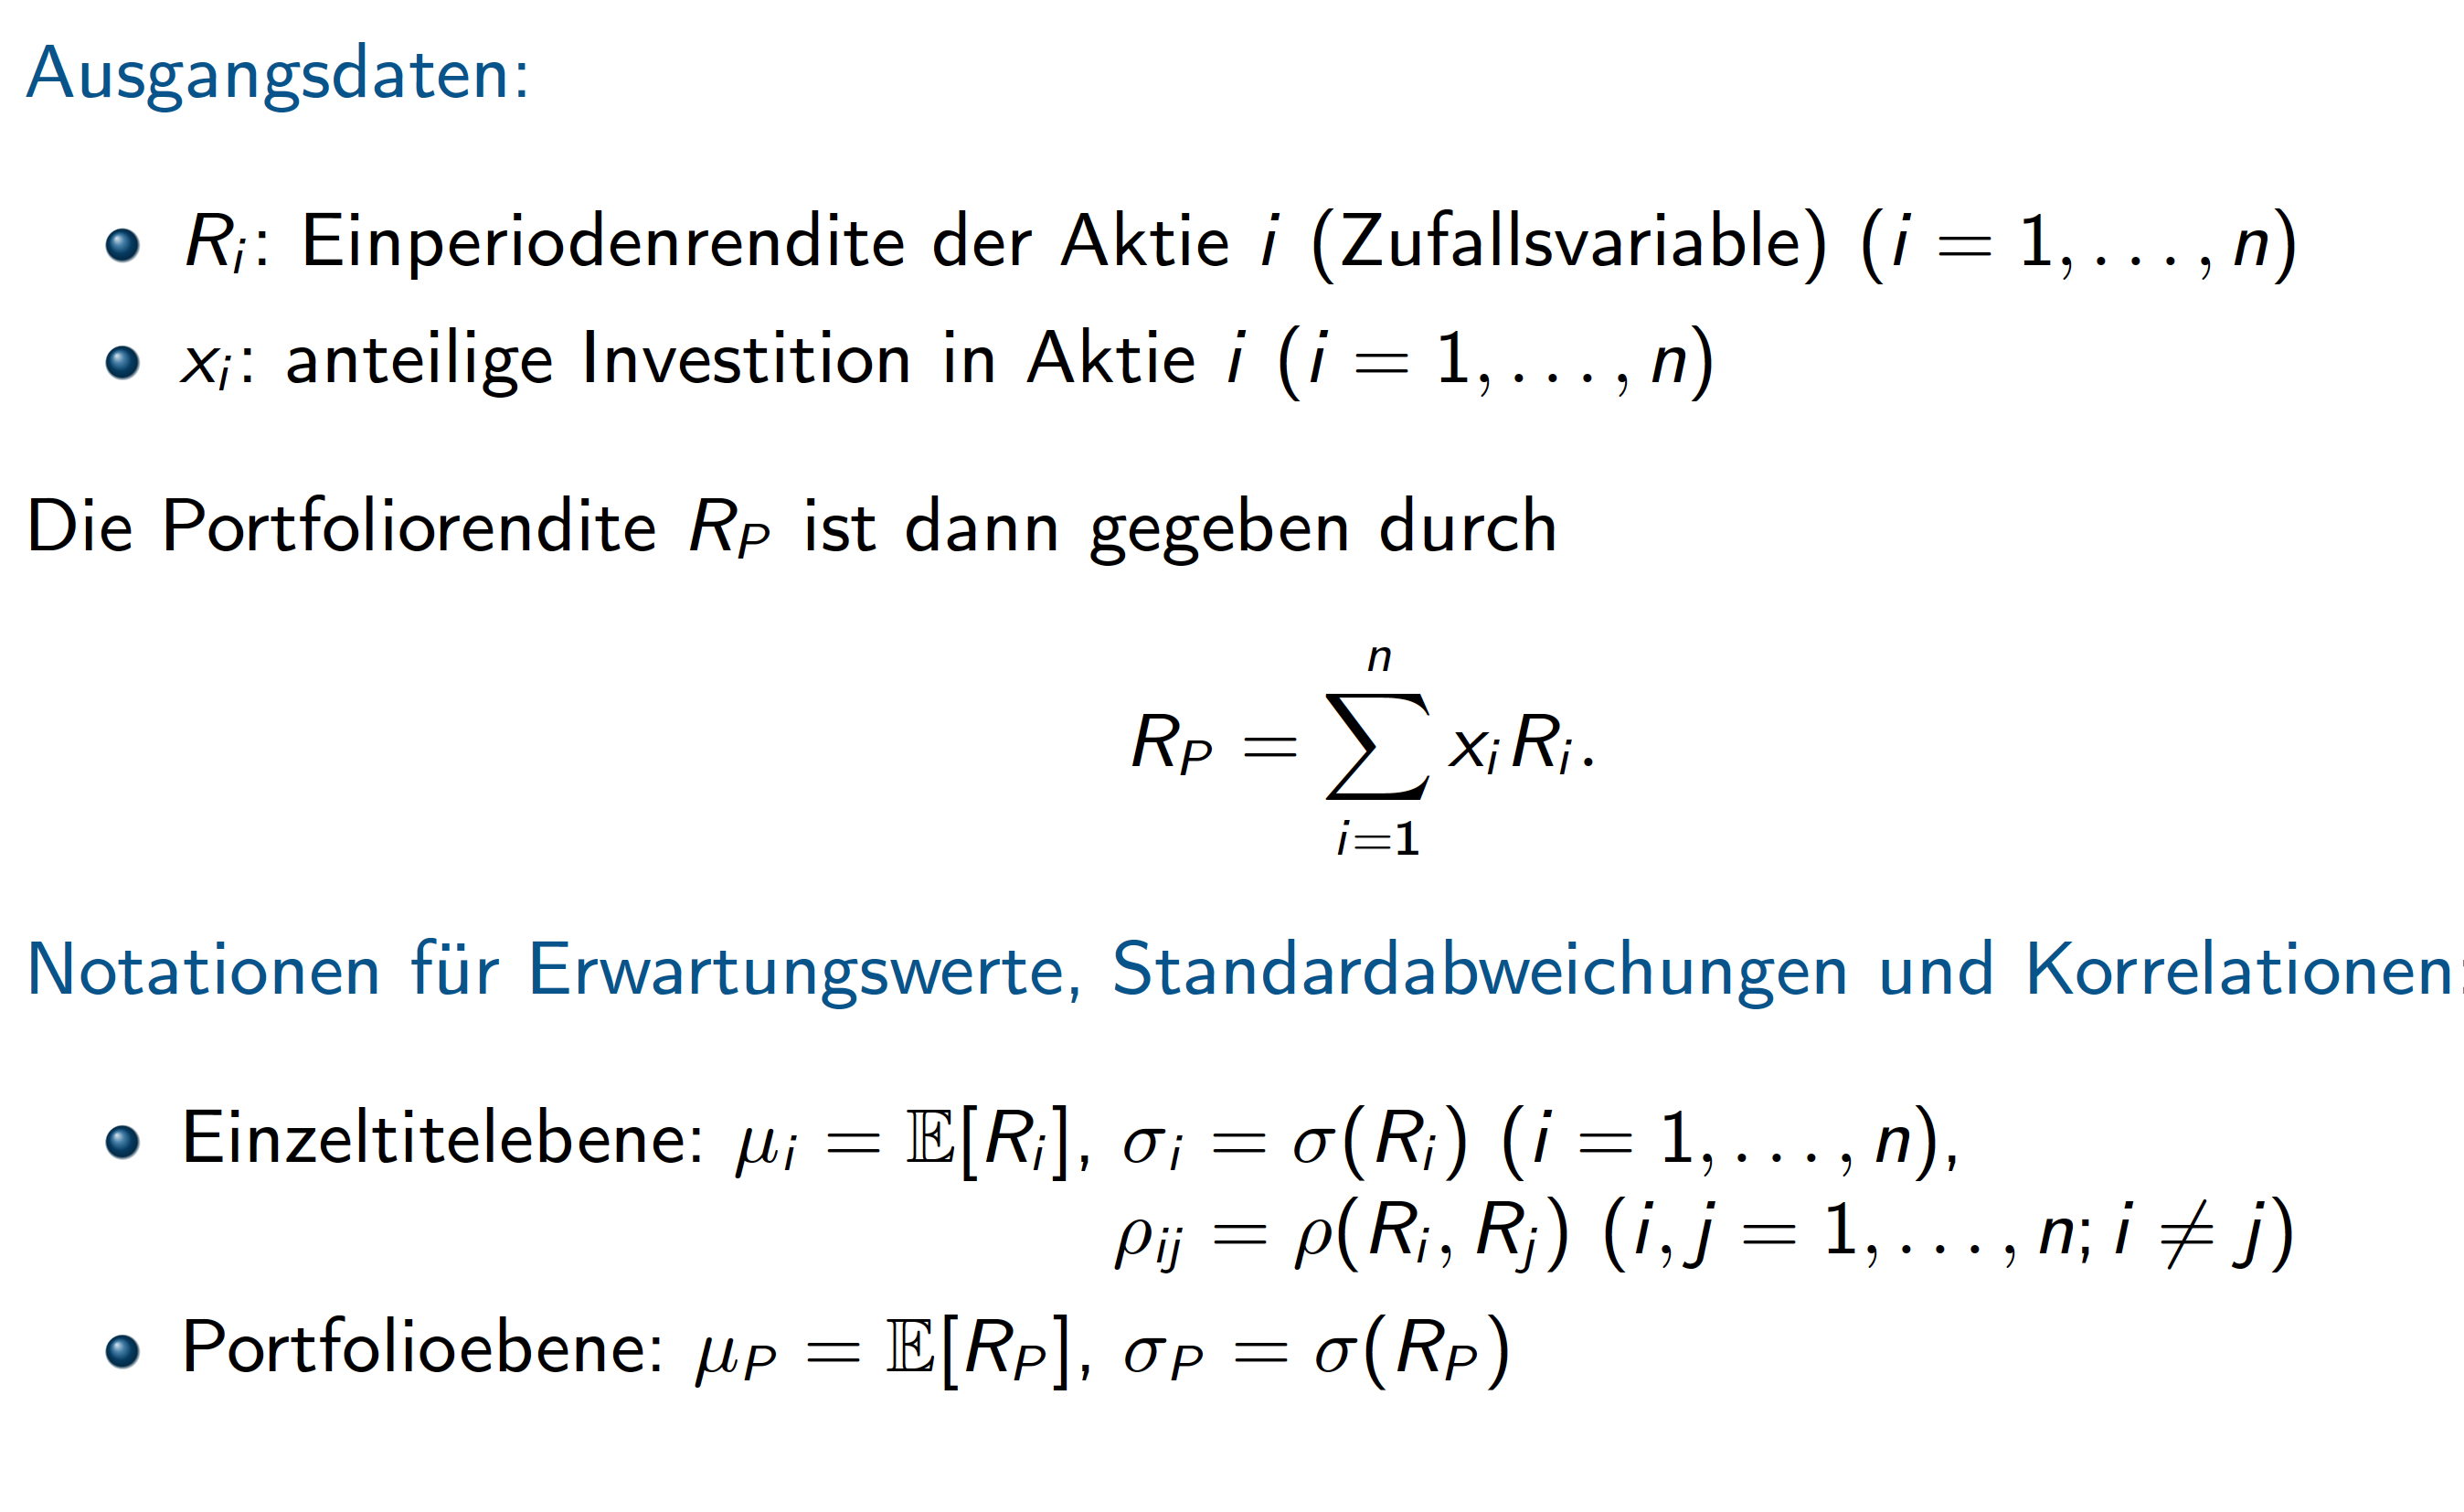
\includegraphics[width=\textwidth]{Bilder/Ausgangsdaten.png}
\end{figure}

\subsection{Effiziente Portfolios}

\begin{figure}[H]
\centering
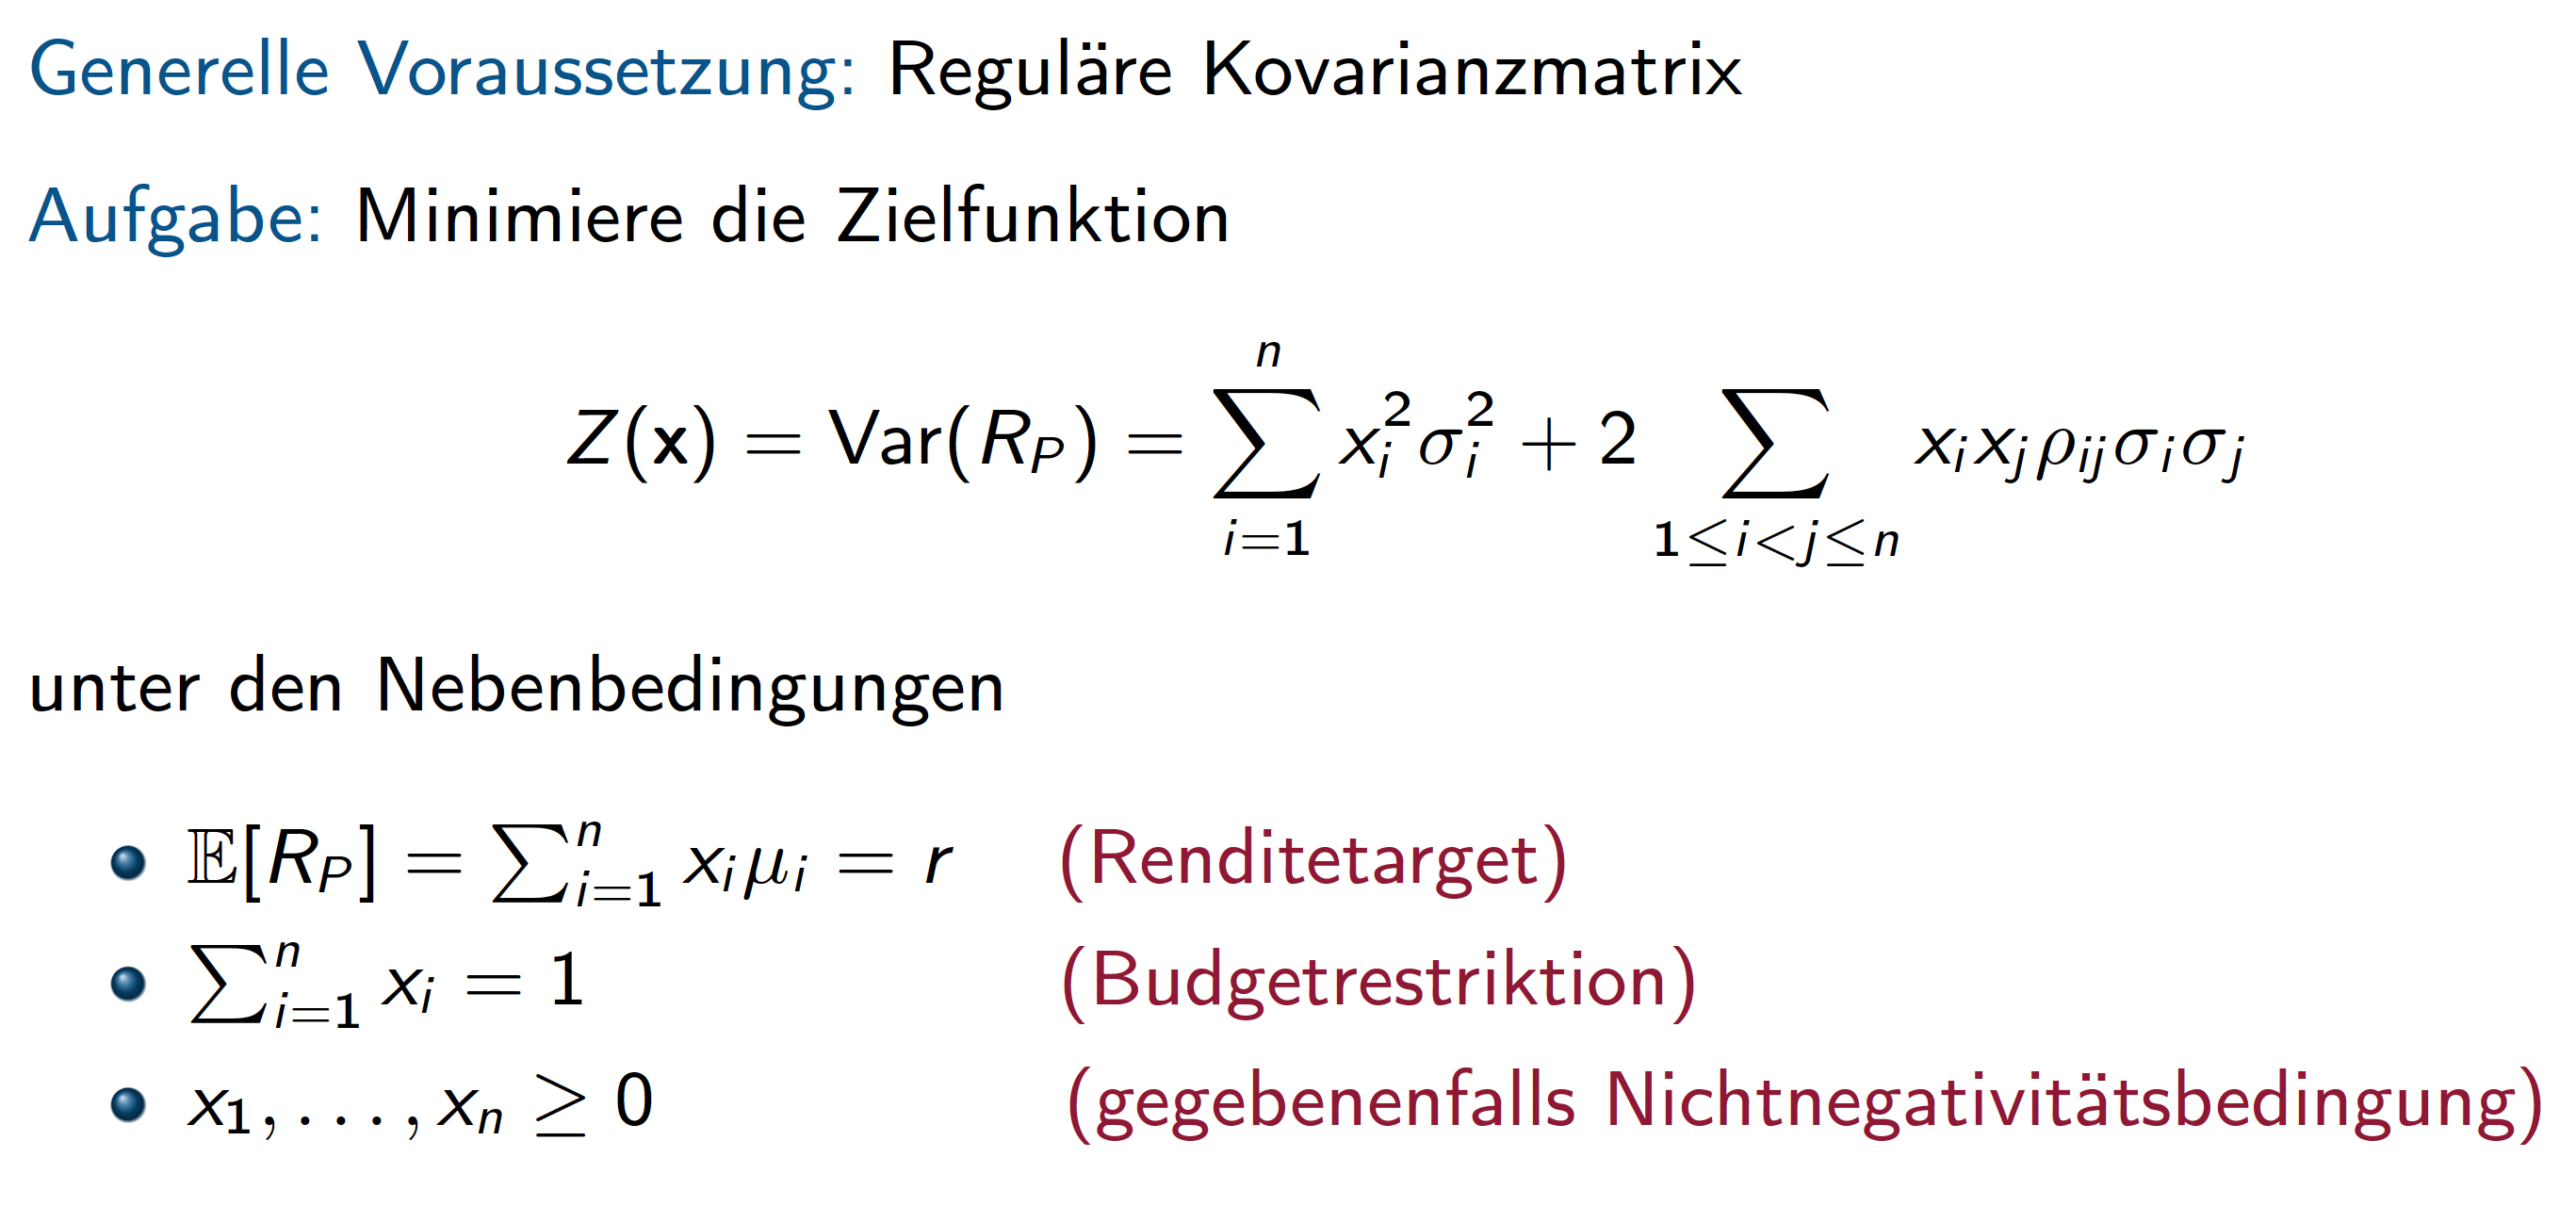
\includegraphics[width=\textwidth]{Bilder/Minimierungsproblem.png}
\end{figure}

\begin{itemize}
	\item Fall 1: Short Sales Allowed, L\"osung mit Lagrange-Ansatz, lokalen Extremwert der Lagrange-Funktion bestimmen
	\begin{itemize}
		\item geometrischer Rand der Menge aller zul\"assigen Portfolios besteht aus den Punkten, die bez\"uglich eines fixierten Erwartungswerts eine minimale Varianz aufweisen
		\item geometrischer Rand ist eine Wurzelfunktion (als Funktion von $\sigma^2$, bzw. der rechte Ast der Hyperbel (als Funktion von $\sigma^2$
		\item der effiziente Rand entspricht dem oberen Ast der Kurve inklusive dem global varianzminimalen Portfolio
	\end{itemize}
	\item Fall 2: No Short Sales, Quadratische Programmierung, i.A. keine analytische L\"osung, numerische Verfahren
\end{itemize}

\subsubsection{Alternative Formulierungen des Problems}

\begin{figure}[H]
\centering
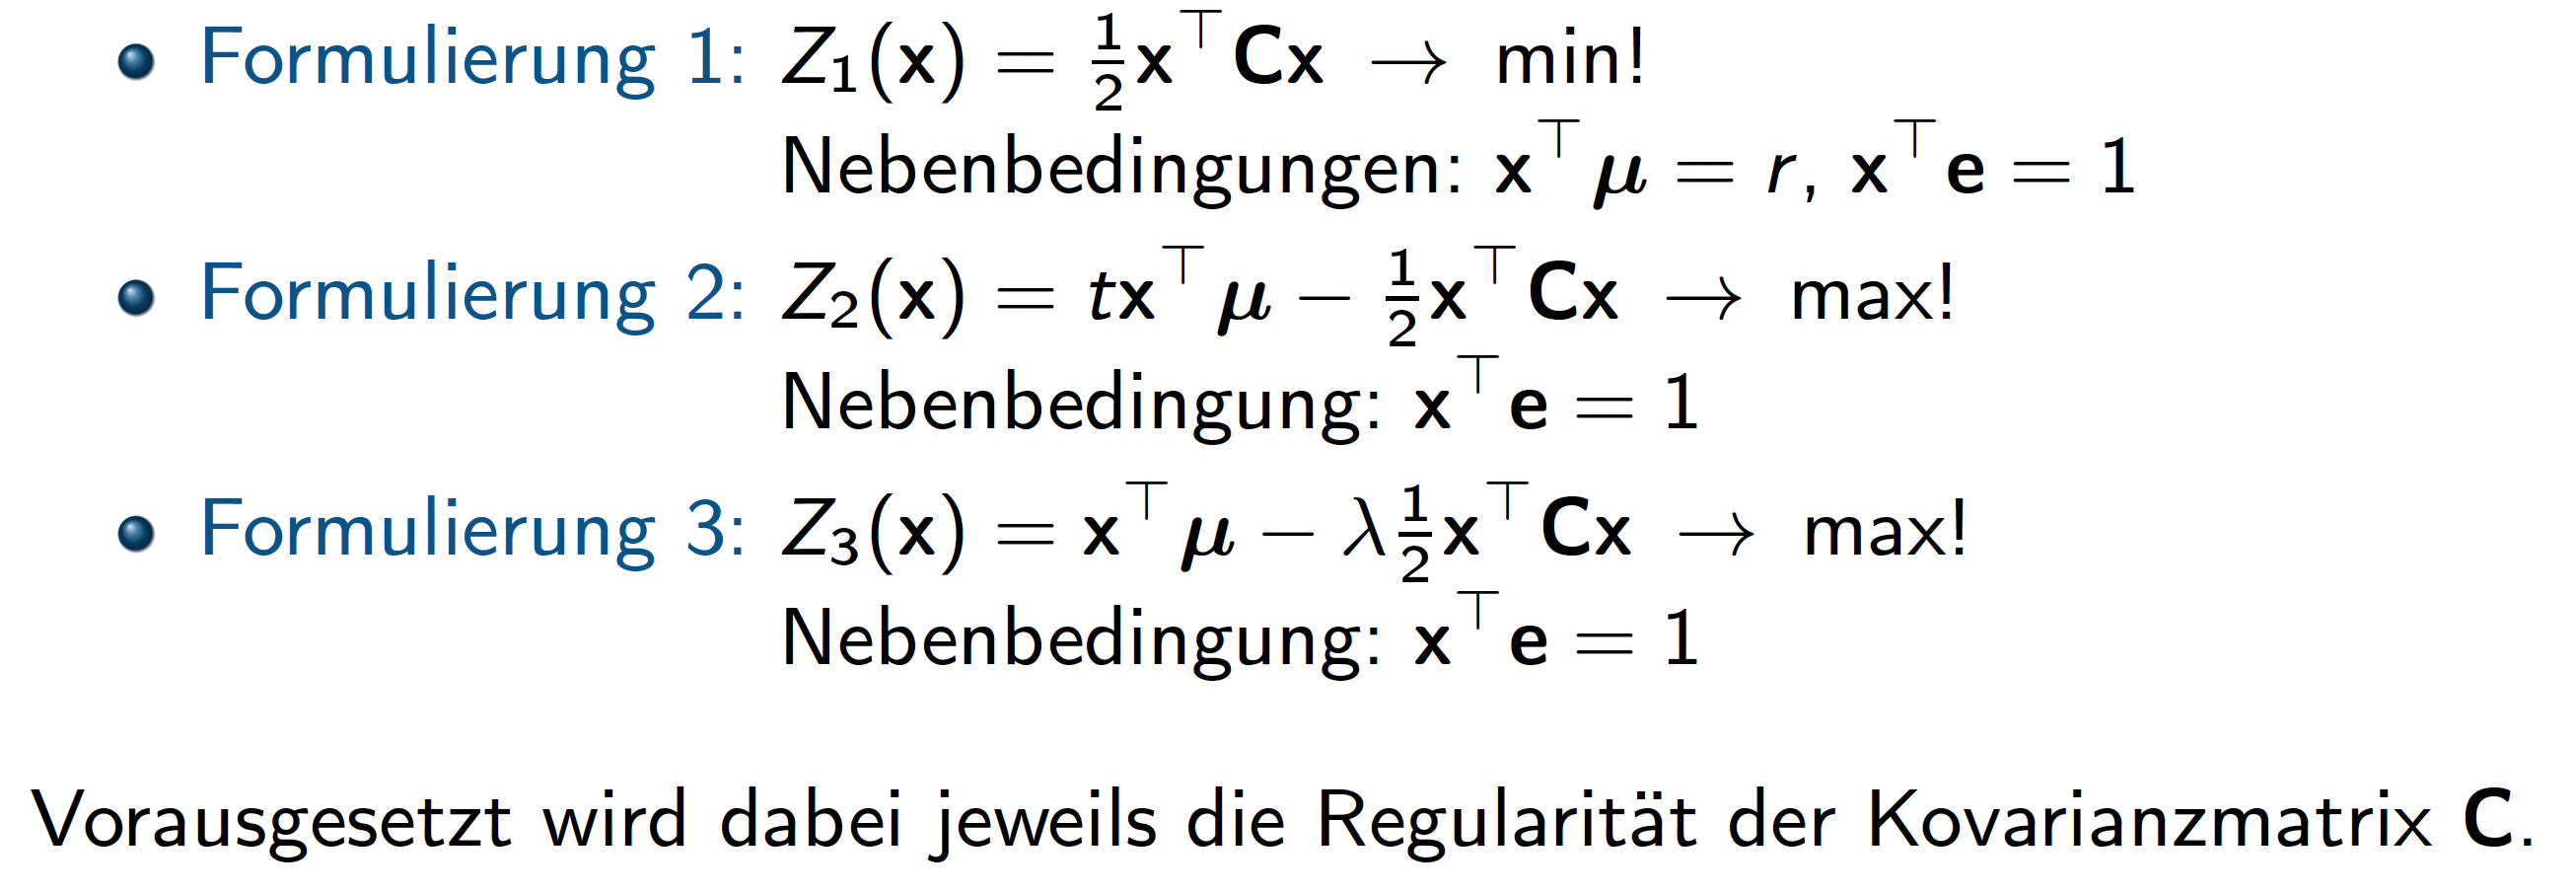
\includegraphics[width=\textwidth]{Bilder/alternativeFormulierungen.png}
\end{figure}

\begin{itemize}
	\item Lagrange-Funktion f\"ur Formulierung 2: \\ $L(x, \lambda) = tx^T \mu - \frac{1}{2} x^T Cx - \lambda (x^T e - 1)$ 
	\item $\sigma^2 = \sigma_0^2 + \frac{1}{\alpha_1}(\mu - \mu_0)^2$
	\item $\mu = \mu_0 \pm \sqrt{\alpha_1 (\sigma^2 - \sigma_0^2) }$
\end{itemize}



\subsection{Portfolioselektion}

\begin{itemize}
	\item Trade-Off zwischen Risiko und Rendite, d.h. Selektion einer charakteristischen $(\sigma, \mu)$-Position auf dem effizienten Rand
	\item Spezifizierung einer EV-Pr\"aferenzfunktion: $\mathcal{U}(R)=H(\mathbb{E}[R], \sigma(R))$
	\item Optimierungsproblem: $H(\mu, \sigma) = V(x_1,...,x_n) \rightarrow max$, Nebenbed.: $(\sigma, \mu) \in M, (x_1,...,x_n) \in D$ mit M Menge der zul\"assigen $(\mu, \sigma)$-Positionen bzw. $D$ die Menge der zul\"assigen Investmentgewichte
\end{itemize}

\subsection{Probleme des Markowitz-Ansatzes}

\begin{itemize}
	\item Markowitz-Basismodell beruht auf Risikoma{\ss} Standardabweichung (vor allem f\"ur symmetrische Verteilungen, in der Praxis aber oft signifikante Schiefe vorhanden)
	\item Optimierte Portfolios besitzen oftmals extreme Allokationen (hohe Leerverkaufspositionen oder geringe Diversifikation, optimale Portfolios \"ubergewichten Assets, die hohe gesch\"atzte erwartete Renditen und geringe Varianzen aufweisen)
	\item Optimierung sehr sensitiv bez\"uglich Inputdaten
\end{itemize}

\section{Alternative Ans\"atze der Portfoliooptimierung}

\begin{itemize}
	\item Markowitz-Modell: Standardabweichung als Risikoma{\ss}
	\item jetzt andere Risikoma{\ss}e verwenden
	\item Value at Risk:
	\begin{itemize}
		\item nicht subadditiv
		\item Portfoliorisiko $V@R_{\lambda}(R_P(x))$ i.A. keine konvexe Funktion
	\end{itemize}
	\item Average Value at Risk
	\begin{itemize}
		\item lageabh\"angiges Risikoma{\ss} (auch Mean-AV@R und Mean-V@R in der Literatur betrachtet)
		\item Generelle Form: $AV@R_{\lambda}(R_P(x)) \rightarrow min$
		\item Nebenbedingungen:
		\item[1.] $E[R_P(x)] = r$
		\item[2.] $x^Te = 1$
		\item[3.] $x \geq 0$ 
		\item $AV@R_{\lambda}(X) = V@R_{\lambda}(X) + \frac{1}{\lambda} \mathbb{E}[(-X-V@R_{\lambda}(X))^{+}]$
	\end{itemize}
\end{itemize}

\section{Asset Pricing}

\subsection{Portfoliotheorie mit sicherer Anlage}

\subsubsection{Erweiterung des Anlagespektrums}
\begin{itemize}
	\item Risikolose Anlage (Renditevarianz = 0) zum sicheren Zins $r_0$
	\item vollkommener Kapitalmarkt: zum Zins $r_0$ k\"onnen beliebige Betr\"age angelegt oder aufgenommen werden
\end{itemize}

\subsubsection{Elementare Analyse}
\begin{itemize}
	\item fixiere riskantes Portfolio $P \in M$, d.h. Portfolio aus der Menge der durch Aktienmischung realisierbaren Portfolios
	\item Betrachte Portfolio, das z.T. in sichere Anlagen investiert und zum Teil in $P$
	\item $R_P$ ist die Rendite von $P$
	\item $0 \leq x \leq \infty$ anteilige Investition in $P$
	\item $-\infty < 1-x \leq 1$ anteilige in Investition in sichere Anlage
	\item Rendite gesamt: $R=xR_P + (1-x)r_0$
	\item $\mu = r_0+x(\mu_P - r_0)$
	\item $\sigma^2 = x^2 \sigma_P^2$
	\item[$\Rightarrow$] $\mu = r_0 + \frac{\mu_P-r_0}{\sigma_P}\sigma$
	\item Menge aller effizienten bzw. optimalen Portfolios ist eine Gerade (Tangentialgerade an den bisherigen effizienten Rand 
\end{itemize}

\subsection{Capital Asset Pricing Model}

\subsubsection{Pr\"amissen des CAPM}
\begin{itemize}
	\item Fall $r_0 < \mu_0$
	\item Es gibt $m$ EV-Investoren mit Wertpapierbudgets $V_i >0$, $V = \sum_{i=1}^m V_i$
	\item alle Investoren sch\"atzen $r_0$, $\mathbb{E}[R_i]$, $Var(R_i)$ und $Cov(R_i,R_j)$ gleich ein
	\item Marktgleichgewicht (Angebot = Nachfrage)
\end{itemize}

\subsubsection{Marktportfolio}
\begin{itemize}
	\item jeder Investor erwirbt EV-effizientes Portfolio, Anteil $\lambda_i$ des Budgets $V_i$ in Tangentialportfolio, Rest ($1-\lambda_i$) in sichere Anlage
	\item Nachfrageportfolio des Marktes nach Aktien: $(\lambda^T V)x_T$
	\item Angebotsportfolio: alle Aktien, die zu $t=0$ zu Marktwerten bewertet werden
\end{itemize}

\begin{figure}[H]
\centering
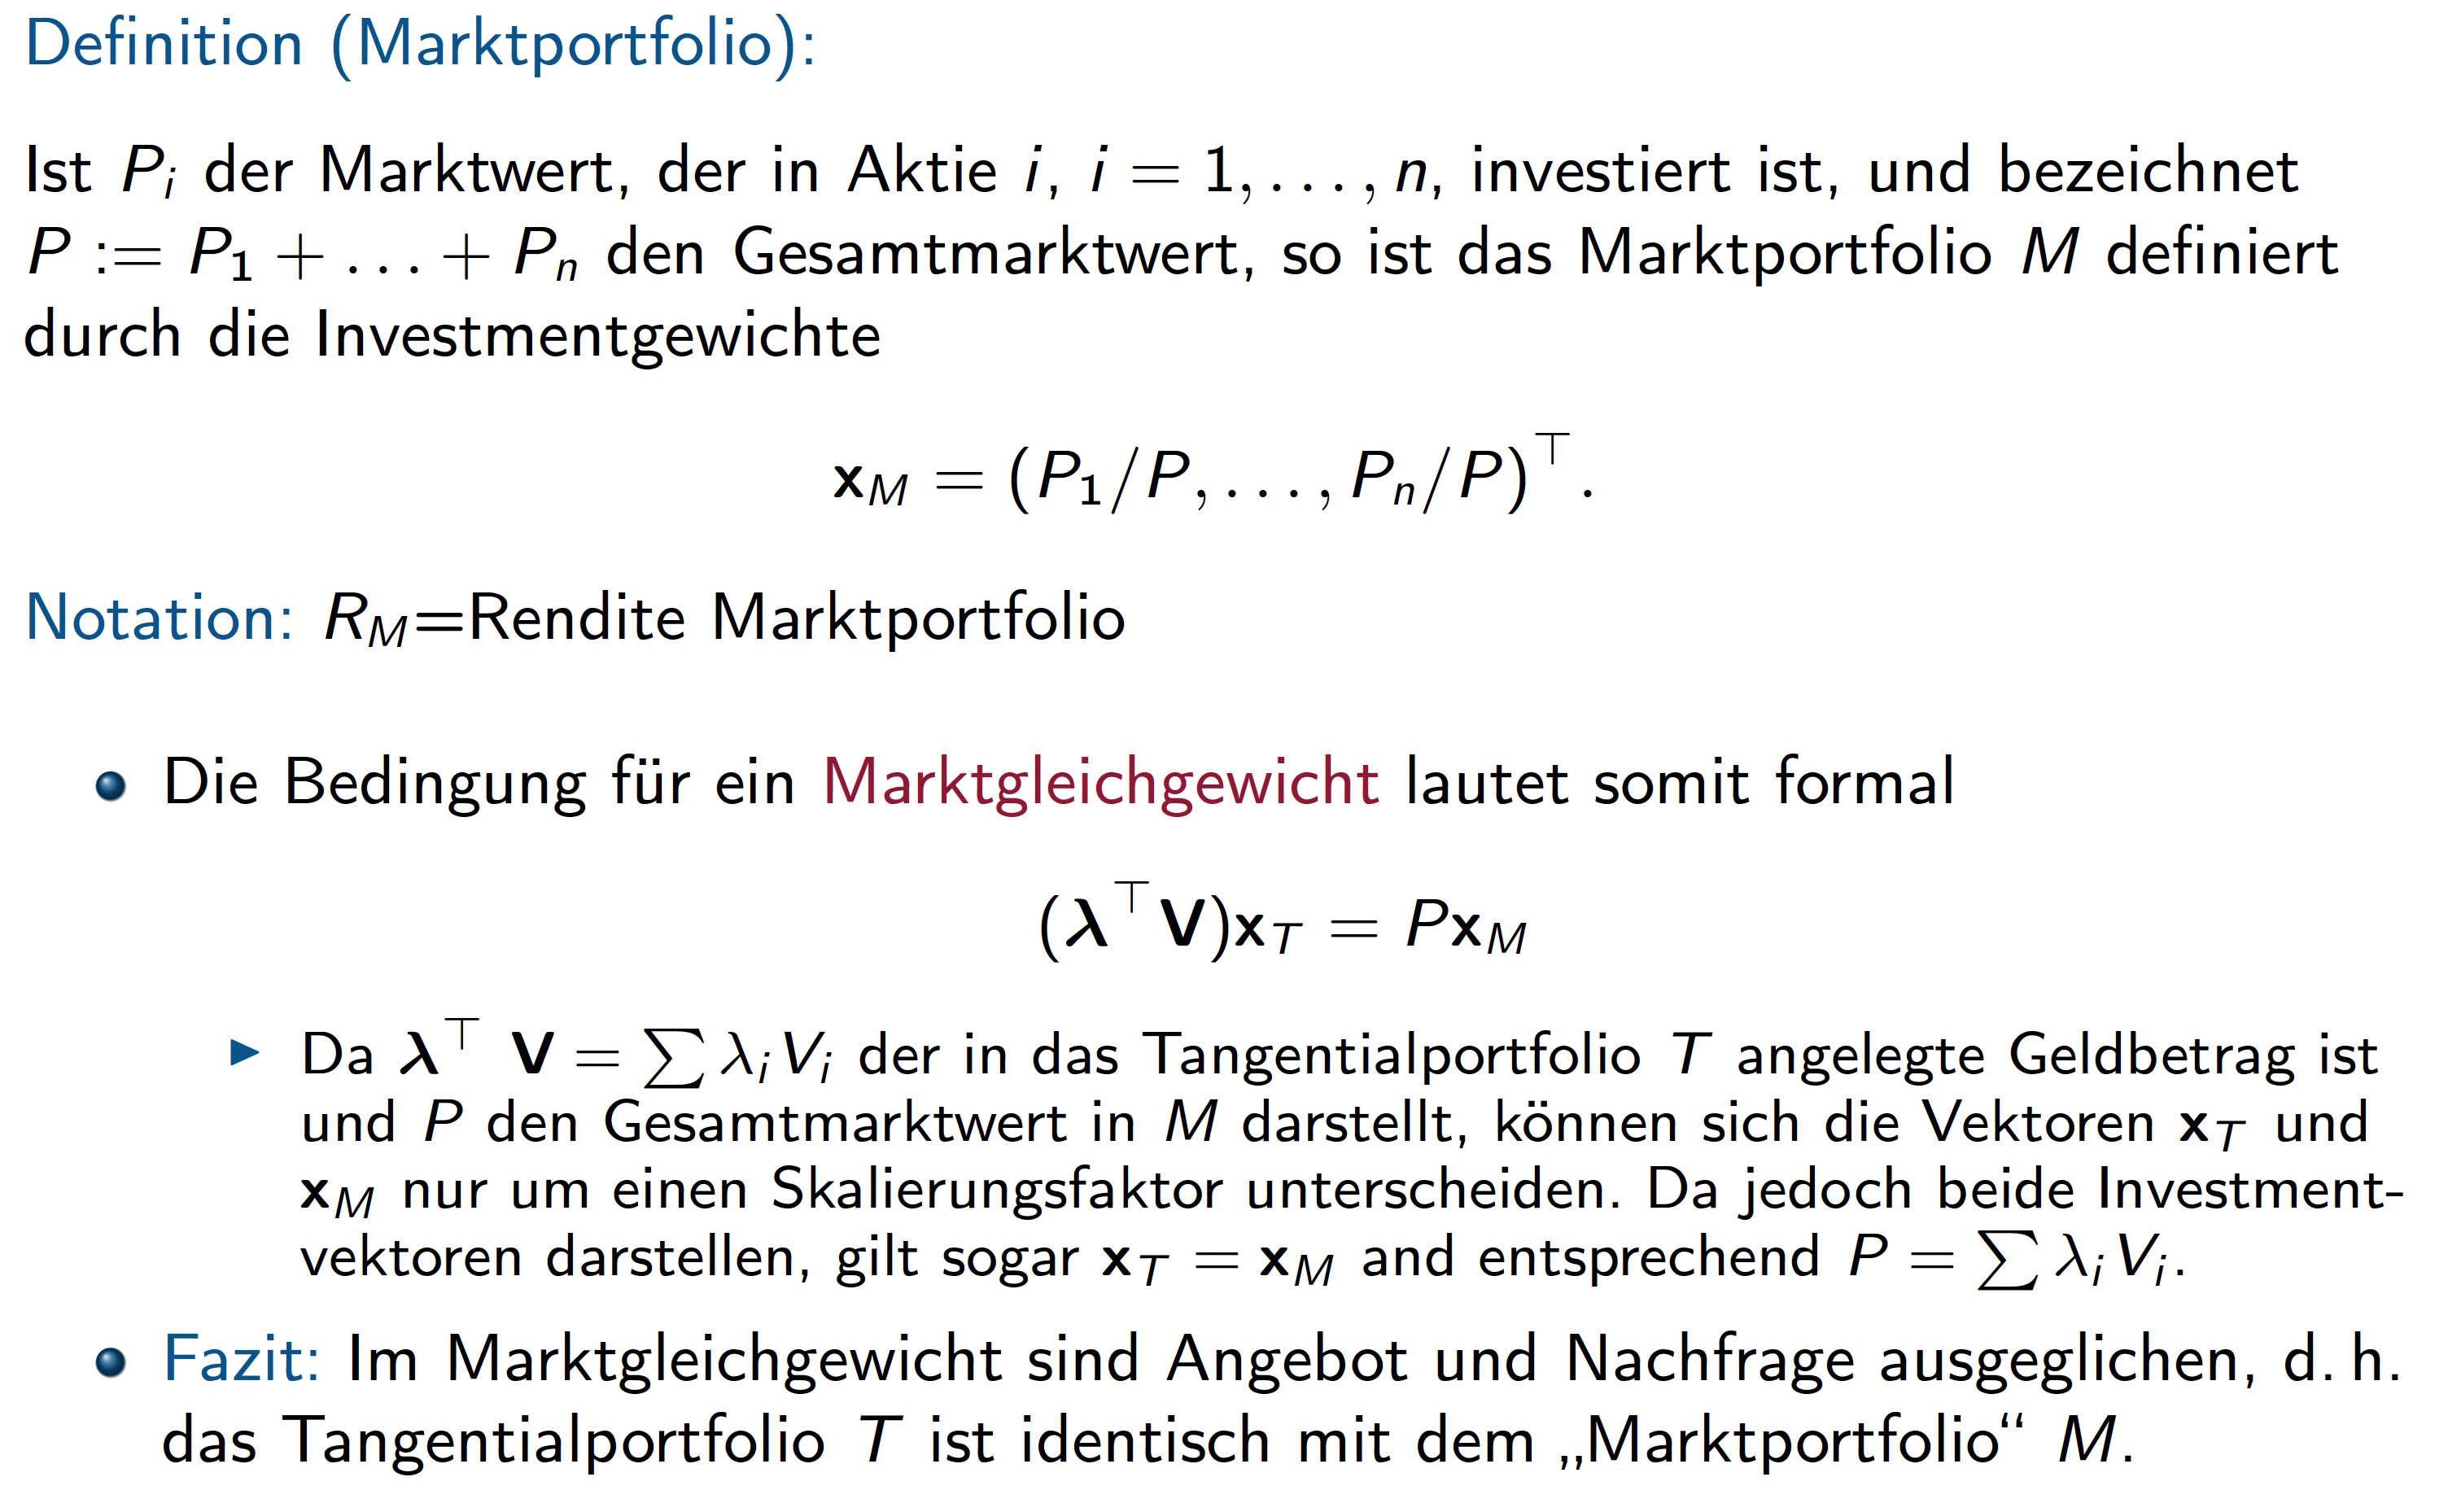
\includegraphics[width=\textwidth]{Bilder/Marktportfolio.png}
\end{figure}

\subsubsection{CAPM-Analytik}

\begin{figure}[H]
\centering
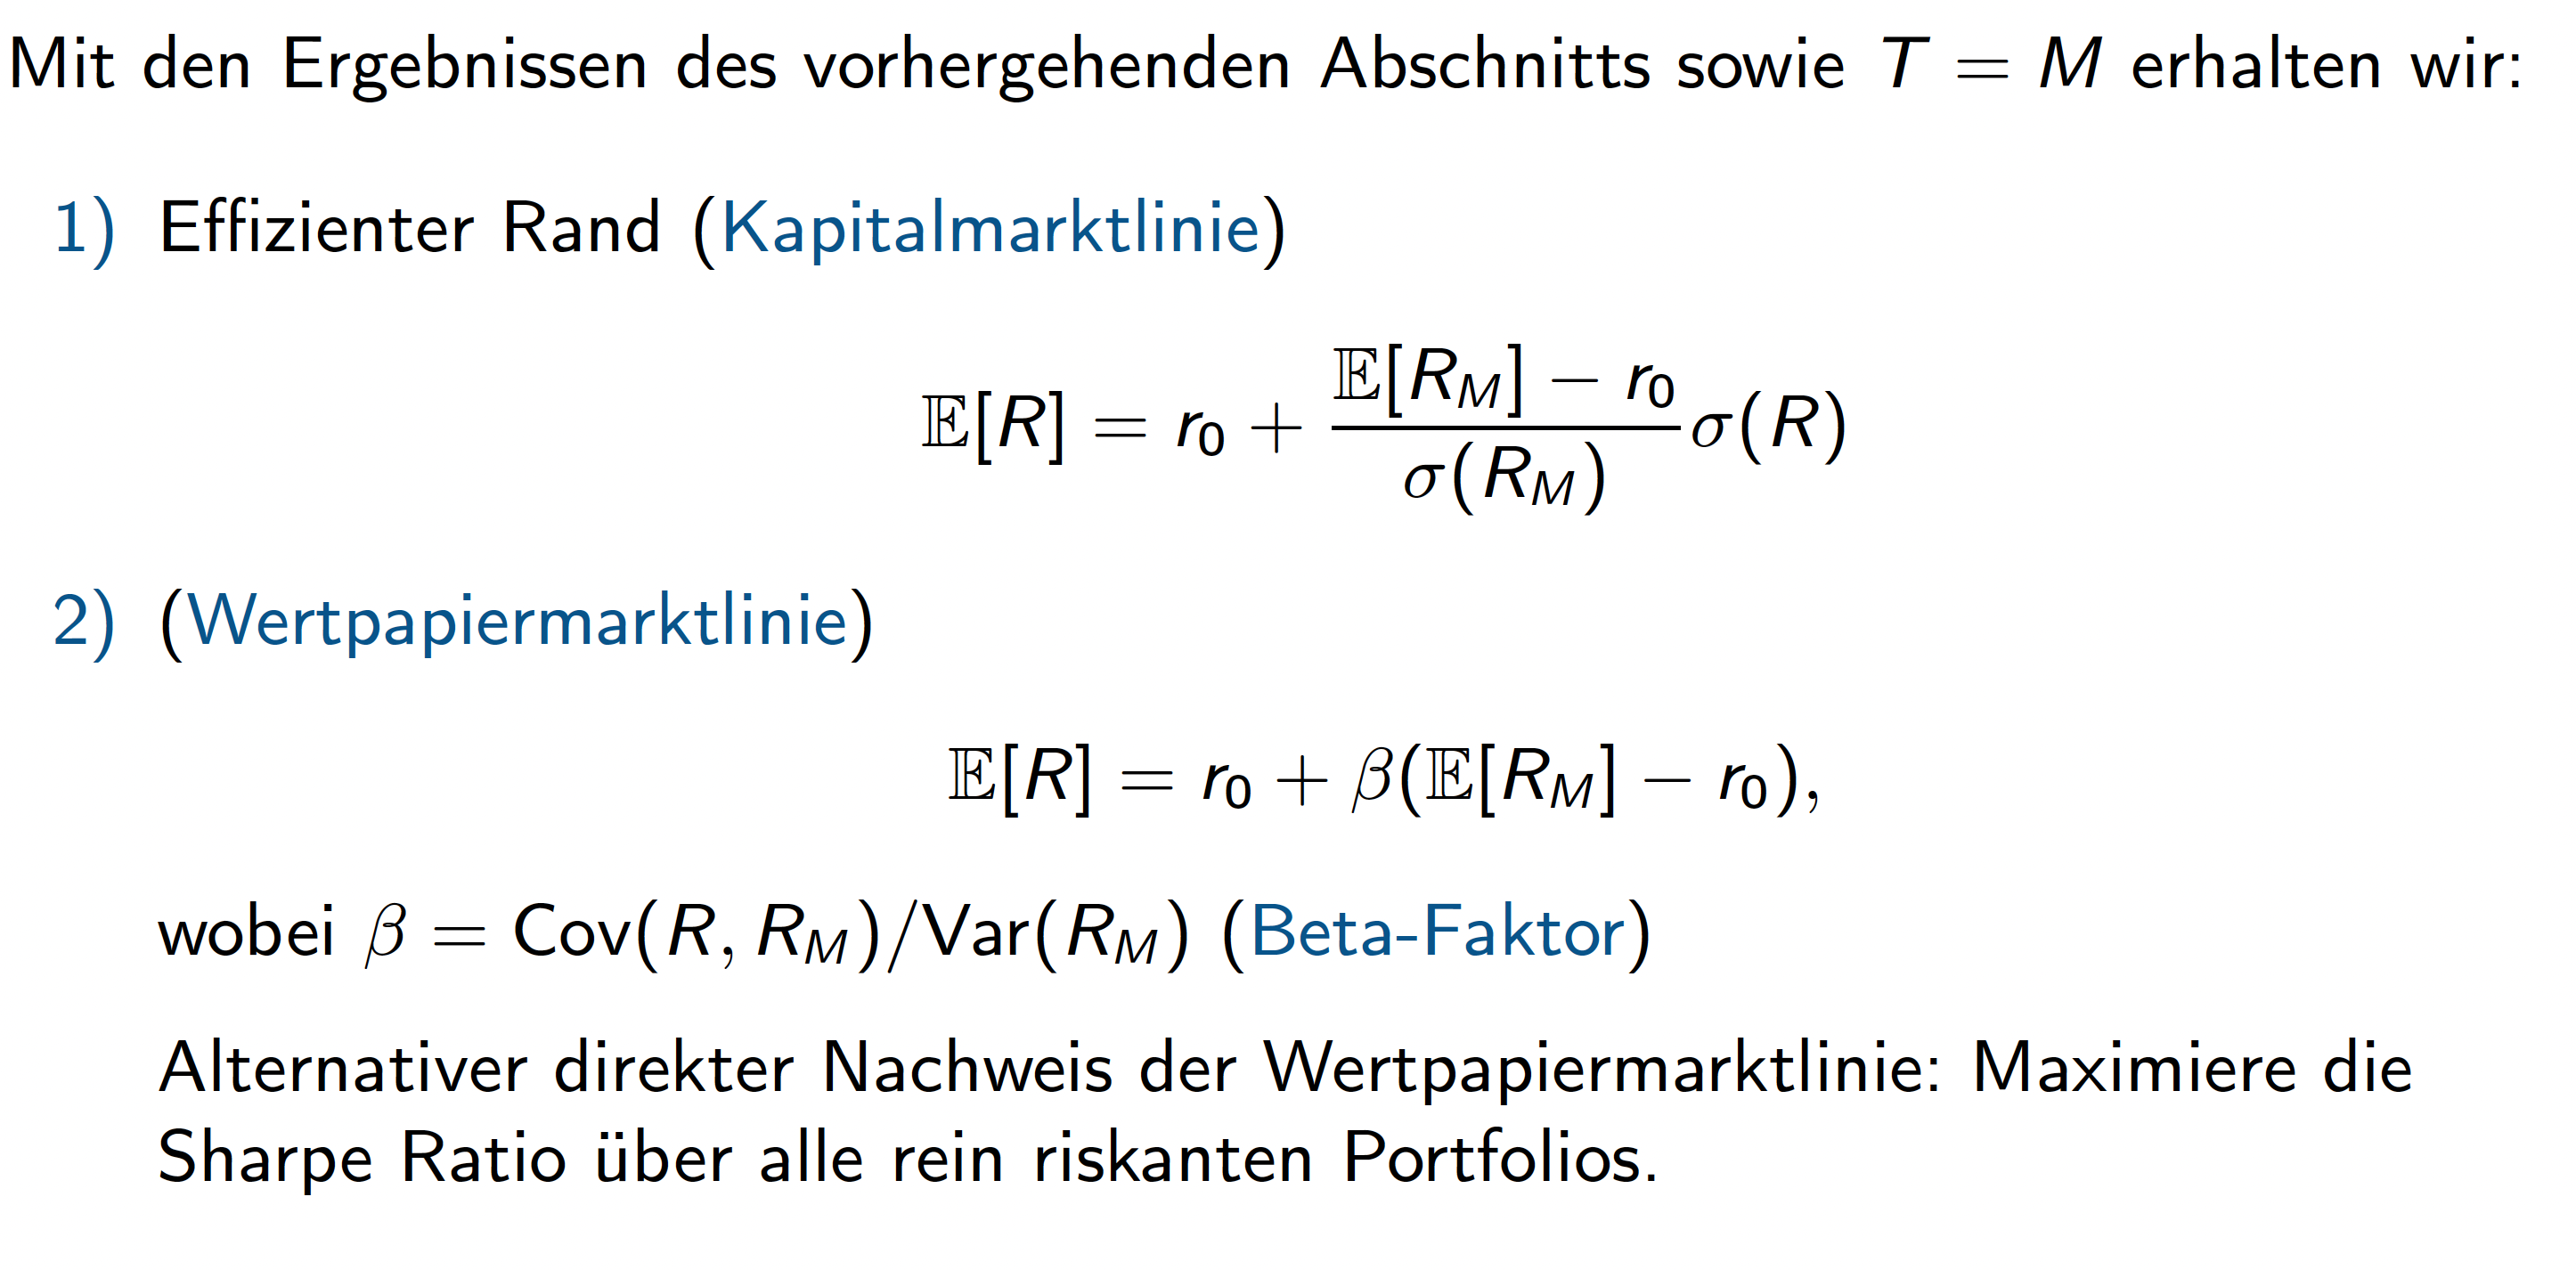
\includegraphics[width=\textwidth]{Bilder/CAPMAnalytik.png}
\end{figure}

\subsubsection{Hauptresultate des CAPM}

\begin{itemize}
	\item Menge aller optimalen Portfolios $R$ (Kapitalmarktlinie): $\mathbb{E}[R] = r_0 + \frac{\mathbb{E}[R_M] - r_0}{\sigma(R_M)}\sigma(R)$
	\item Menge aller optimalen Portfolios $R$ (Wertpapiermarktlinie): $\mathbb{E}[R] = r_0 + \beta_R(\mathbb{E}[R_M] - r_0)$ mit $\beta_R = \frac{Cov(R,R_M)}{Var(R_M)}$
	\item Preisgleichung $P= \frac{\mathbb{E}[V]}{1+r_0+\beta(\mathbb{E}[R_M]-r_0)}$ 
	\item $P$ der anf\"anglichen Preisen eines Titels mit zufallsabh\"angigem Endwert $V$ und korrespondierender Einperiodenrendite $R$
	\item $r_0$ sicherer Zins
	\item $R_M$ Rendite des Marktportfolios
\end{itemize}










































\end{document}